\documentclass[a4paper, twoside]{report}

%% Language and font encodings
\usepackage[english]{babel}
\usepackage[utf8x]{inputenc}
\usepackage[T1]{fontenc}

%% Sets page size and margins
\usepackage[a4paper,top=3cm,bottom=2cm,left=3cm,right=3cm,marginparwidth=1.75cm]{geometry}

%% Useful packages
\usepackage{amsmath}
\usepackage{mathtools}
\usepackage{amssymb}
\usepackage{graphicx}
\usepackage{listings}
\usepackage{float}
\usepackage{xcolor}
\usepackage{multicol}
\usepackage{backnaur}
\usepackage{geometry}
\usepackage{longtable}
\usepackage{array}
\usepackage{tcolorbox}
\usepackage{fancyvrb}
\usepackage{framed}
\usepackage{pifont}
\newcommand{\cmark}{\ding{51}}%
\newcommand{\xmark}{\ding{55}}%
\usepackage{booktabs}
\usepackage[colorinlistoftodos]{todonotes}
\usepackage[colorlinks=true, allcolors=blue]{hyperref}

% Code blocks
\definecolor{dkgreen}{RGB}{0,128,0} % Define the dkgreen color using RGB values
\lstset{
  frame=none,
  language=Promela,
  aboveskip=5mm,
  belowskip=5mm,
  showstringspaces=false,
  columns=flexible,
  xleftmargin=.3\textwidth,
  basicstyle={\small\ttfamily},
  numbers=none,
  numberstyle=\tiny\color{gray},
  keywordstyle=\color{blue},
  commentstyle=\color{dkgreen},
  stringstyle=\color{orange},
  breaklines=true,
  breakatwhitespace=true,
  tabsize=3,
  numbers=left, 
  captionpos=b, 
}

% Elixir code colouring
\definecolor{commentgreen}{RGB}{2,112,10}
\definecolor{eminence}{RGB}{108,48,130}
\definecolor{weborange}{RGB}{255,165,0}
\definecolor{frenchplum}{RGB}{129,20,83}

\lstdefinelanguage{elixir}{
    morekeywords={case,catch,def,defv,pre,post,do,else,false,%
        use,alias,receive,timeout,defmacro,defp,%
        for,if,import,defmodule,defprotocol,%
        nil,defmacrop,defoverridable,defimpl,%
        super,fn,raise,true,try,end,with,%
        unless, quote, unquote},
    otherkeywords={<-,->, |>, \%\{, \}, \{, \, (, )},
    sensitive=true,
    morecomment=[l]{\#},
    morecomment=[n]{/*}{*/},
    morecomment=[s][\color{purple}]{:}{\ },
    morestring=[s][\color{orange}]"",
    commentstyle=\color{commentgreen},
    keywordstyle=\color{eminence},
    stringstyle=\color{red},
	basicstyle=\ttfamily,
	breaklines,
	showstringspaces=false,
	frame=none,
    escapeinside={(*@}{@*)}
}
\lstdefinestyle{promela}{
    language=C,
    morekeywords={proctype, init, chan},
    keywordstyle=\color{blue},
    commentstyle=\color{gray},
    stringstyle=\color{orange},
    basicstyle=\ttfamily\footnotesize,
    showstringspaces=false,
    breaklines=true,
    frame=single,
    captionpos=b,
    tabsize=2
}
\lstdefinelanguage{dafny}{
    morekeywords={method, function, class, var, assert, ensures, requires, modifies, decreases, new, if, else, while, break, return, ghost, forall, exists, invariant, axiom, datatype},
    sensitive=true,
    morecomment=[l]{//},
    morecomment=[s]{/*}{*/},
    morestring=[b]",
    commentstyle=\color{green},
    keywordstyle=\color{blue},
    stringstyle=\color{red},
    basicstyle=\ttfamily,
    breaklines,
    showstringspaces=false,
    frame=none
}
\lstdefinelanguage{boogie}{
    morekeywords={implementation, procedure, assert, assume, havoc, call, return, var, function, modifies, ensures, requires, if, else, while, break, continue},
    sensitive=true,
    morecomment=[l]{//},
    morecomment=[s]{/*}{*/},
    morestring=[b]",
    commentstyle=\color{green},
    keywordstyle=\color{blue},
    stringstyle=\color{red},
    basicstyle=\ttfamily,
    breaklines,
    showstringspaces=false,
    frame=none
}
\lstdefinelanguage{none}{}

\title{Verlixir: Verification of Message-Passing Systems}
\author{Matthew Neave}
% Update supervisor and other title stuff in title/title.tex

\begin{document}
\begin{titlepage}

\newcommand{\HRule}{\rule{\linewidth}{0.5mm}} % Defines a new command for the horizontal lines, change thickness here

%----------------------------------------------------------------------------------------
%	LOGO SECTION
%----------------------------------------------------------------------------------------


\includegraphics[width=8cm]{title/logo.eps}\\[1cm] % Include a department/university logo - this will require the graphicx package
 
%----------------------------------------------------------------------------------------

\center % Center everything on the page

%----------------------------------------------------------------------------------------
%	HEADING SECTIONS
%----------------------------------------------------------------------------------------

\textsc{\LARGE MEng Individual Project}\\[1.5cm] % Name of your university/college
\textsc{\Large Imperial College London}\\[0.5cm] % Major heading such as course name
\textsc{\large Department of Computing}\\[0.5cm] % Minor heading such as course title

%----------------------------------------------------------------------------------------
%	TITLE SECTION
%----------------------------------------------------------------------------------------
\makeatletter
\HRule \\[0.4cm]
{ \huge \bfseries \@title}\\[0.4cm] % Title of your document
\HRule \\[1.5cm]
 
%----------------------------------------------------------------------------------------
%	AUTHOR SECTION
%----------------------------------------------------------------------------------------

\begin{minipage}{0.4\textwidth}
\begin{flushleft} \large
\emph{Author:}\\
\@author % Your name
\end{flushleft}
\end{minipage}
~
\begin{minipage}{0.4\textwidth}
\begin{flushright} \large
\emph{Supervisor:} \\
Dr. Naranker Dulay \\[1.2em] % Supervisor's Name
\emph{Second Marker:} \\
TBD % second marker's name
\end{flushright}
\end{minipage}\\[2cm]
\makeatother

% If you don't want a supervisor, uncomment the two lines below and remove the section above
%\Large \emph{Author:}\\
%Matthew \textsc{Neave}\\[3cm] % Your name

%----------------------------------------------------------------------------------------
%	DATE SECTION
%----------------------------------------------------------------------------------------

{\large \today}\\[2cm] % Date, change the \today to a set date if you want to be precise

\vfill % Fill the rest of the page with whitespace

\end{titlepage}

\begin{abstract}
    Distributed algorithms are difficult to prove and reason about. With the rapid rise in cloud-based clusters the need for developing robust distributed algorithms is seen as a critical requirement by service providers and has sparked new interest in developing tools for reasoning about distributed algorithms.
    \\ \\
    This project proposes and evaluates Verlixir, a verification-aware language for specifying and verifying message-passing systems. Verlixir supports three modes of operation. Simulation mode can be used to execute and observe the system in a controlled environment. Verification mode can be used to verify the system against a set of properties. Finally, parameterization mode can be used to guarantee the system behaves across different configurations.
    \\ \\
    A qualitative evaluation of Verlixir demonstrates capability to detect violations of properties in distributed algorithms, such as, Paxos and Two-Phase Commit. Verlixir enhances Elixir programs with linear temporal logic properties, predicates and function contracts to specify the desired behaviour of systems. Property violations produce Elixir-friendly counterexamples that can be used to debug the system. Counterexamples show process interleaving as well as message-passing interleaving that results in a property violation.
    \\ \\
    Verlixir enables developers to define message-passing systems in terms of safety and liveness. Distributed algorithms can be prototyped and verified in a safe environment. Verlixir replaces the need for writing complex models in bespoke specification languages, which have to be maintained alongside implementation in modern programming languages. This is all achieved while maintaining the original program semantics, such that, after verification, the system can be run in production.
\end{abstract}
\renewcommand{\abstractname}{Acknowledgements}
\begin{abstract}
Thanks mum!
\end{abstract}

\tableofcontents
\listoffigures
\lstlistoflistings
% \listoftables

% \chapter{Introduction}
With the rise of cloud-based clusters, developing robust distributed algorithms is becoming an increasingly difficult problem and the need for vigorous methodologies to verify the correctness of these algorithms has intensified. Modern programming languages have been developed to support distributed algorithms that rely on message-passing as a means of communication between sequential nodes executing in parallel. Common message-passing abstractions involve the use of channels (e.g. Go \cite{go}) or actors \cite{actor} (e.g. Erlang \cite{erlang}). Message-passing abstractions can be simple and more natural to reason about than a common alternative in shared-memory concurrency, however, it can also become more difficult to verify a program implements a given specification.
\par
Verification tools have been developed to support determining the correctness of systems. For example, first-order automated theorem provers such as Z3 \cite{z3} and formal specification languages like TLA+ \cite{tlaplus}. These tools allow systems to be modelled, and specifications to be defined that can then be used to prove properties over these systems. However, despite the power these tools provide, they often place a burden on developers to write and maintain models of systems alongside their actual implementation. This often leads to a paradigm shift away from system implementations that were designed in, for example, imperative programming languages such as C. Modern programming languages such as Dafny \cite{dafny} solve this issue by directly integrating Floyd-Hoare style logic verification alongside the implementation.
\par
Elixir \cite{elixir} is a functional programming language built on top of Erlang that runs on the BEAM virtual machine \cite{beam}. It is commonly used for building distributed, fault-tolerant applications because it supports concurrency, communication and distribution. Elixir actors are uniquely identified with a process identifier (pid) and associated with an unbounded mailbox. Each mailbox supports communication between actors; one actor can send a message to another actor's mailbox, which is then enqueued and can be received in a First-In-First-Firable-Out (FIFFO) ordering. FIFFO is similar to First-In-First-Out (FIFO) where elements are dequeued in the order they are enqueued, however, Elixir supports receiving messages with pattern-matching such that messages are received in a FIFO order concerning a certain pattern.
\par
This report discusses the automatic modelling of actor-based programs and the verification of their adherence to a specification, using Elixir as a target language to support the verification of real-world systems.
\section{Objectives}
Much work has gone into verifying algorithms and programs such as various theorem provers and model checkers. While these tools were initially designed to allow developers to write specifications for how an algorithm should behave in bespoke specification language, more recently verification tools have been designed that can be directly applied to programs written in programming languages such as C \cite{}. An even more recent advancement is support for verifying concurrent programs, however much of this work has used global shared memory as an implementation for specifying process communication. This project sets out to accomplish the following objectives:
\begin{itemize}
    \item Design novel modelling techniques for actor-based systems.
    \item Determine how specifications can be succinctly specified for actor-based systems.
    \item Design a toolkit for automation of the model checking and verification processes.
    \item Apply the aforementioned techniques and tooling to real-world systems using Elixir as an implementation of the actor model.
\end{itemize}

\chapter{Introduction}
With the rise of cloud-based clusters, developing robust distributed algorithms is becoming an increasingly difficult problem and the need for vigorous methodologies to verify the correctness of these algorithms has intensified. Modern programming languages have been developed to support distributed algorithms that rely on message-passing as a means of communication between sequential nodes executing in parallel. Common message-passing abstractions involve the use of channels (e.g. Go \cite{go}) or actors \cite{actor} (e.g. Erlang \cite{erlang}). Message-passing abstractions can be simple and more natural to reason about than a common alternative in shared-memory concurrency, however, it can also become more difficult to verify a program implements a given specification.
\par
Verification tools have been developed to support determining the correctness of systems. For example, first-order automated theorem provers such as Z3 \cite{z3} and formal specification languages like TLA+ \cite{tlaplus}. These tools allow systems to be modelled, and specifications to be defined that can then be used to prove properties over these systems. However, despite the power these tools provide, they often place a burden on developers to write and maintain models of systems alongside their actual implementation. This often leads to a paradigm shift away from system implementations that were designed in, for example, imperative programming languages such as C. Modern programming languages such as Dafny \cite{dafny} solve this issue by directly integrating Floyd-Hoare style logic verification alongside the implementation.
\par
Elixir \cite{elixir} is a functional programming language built on top of Erlang that runs on the BEAM virtual machine \cite{beam}. It is commonly used for building distributed, fault-tolerant applications because it supports concurrency, communication and distribution. Elixir actors are uniquely identified with a process identifier (pid) and associated with an unbounded mailbox. Each mailbox supports communication between actors; one actor can send a message to another actor's mailbox, which is then enqueued and can be received in a First-In-First-Firable-Out (FIFFO) ordering. FIFFO is similar to First-In-First-Out (FIFO) where elements are dequeued in the order they are enqueued, however, Elixir supports receiving messages with pattern-matching such that messages are received in a FIFO order concerning a certain pattern.
\par
This report discusses the automatic modelling of actor-based programs and the verification of their adherence to a specification, using Elixir as a target language to support the verification of real-world systems.
\section{Objectives}
Much work has gone into verifying algorithms and programs such as various theorem provers and model checkers. While these tools were initially designed to allow developers to write specifications for how an algorithm should behave in bespoke specification language, more recently verification tools have been designed that can be directly applied to programs written in programming languages such as C \cite{}. An even more recent advancement is support for verifying concurrent programs, however much of this work has used global shared memory as an implementation for specifying process communication. This project sets out to accomplish the following objectives:
\begin{itemize}
    \item Design novel modelling techniques for actor-based systems.
    \item Determine how specifications can be succinctly specified for actor-based systems.
    \item Design a toolkit for automation of the model checking and verification processes.
    \item Apply the aforementioned techniques and tooling to real-world systems using Elixir as an implementation of the actor model.
\end{itemize}

\chapter{Background}
\section[]{Communicating Sequential Processes}
\section[]{Model Checking}
Model checking is the process of determining if a finite-state machine (FSM) is correct under a provided specification. It typically involves enumerating all possible states of an FSM and ensuring the correctness of each state. For example, given a model M and a property $\varphi$, if no state of M violates $\varphi$, then we can say M satisfies $\varphi$. In software development, model checkers are beneficial in providing guarantees for safety-critical systems as well as concurrent systems. Concurrent systems can often cause issues with uncommon instruction execution interleavings that are not easily identifiable until long into a runtime. For example, deadlocks can occur when instructions being run by two processes are dependent on one another making progress. A simple example of a deadlock that can occur is the following interleaving of instructions executed by two processes, $\tau_1$ and $\tau_2$. 
\[
\begin{aligned}
& \tau_1: \text{ acquire lock A} \\
& \tau_2: \text{ acquire lock B} \\
& \tau_1: \text{ acquire lock B} \\
& \tau_2: \text{ acquire lock A}
\end{aligned}
\]
This simple interleaving results in $\tau_1$ blocking until it can acquire lock B, and $\tau_2$ blocking until it can acquire lock A, hence the program is in a deadlock. Due to the nature of concurrent systems, we could run our program and never experience this interleaving of instructions from occurring, hence we could deem our program deadlock-free. By instead abstracting our program as a model, and verifying the correctness using a model checker, we could exhaustively check all possible states (interleavings of concurrent processes) and catch this deadlock. 
\par
Alongside determining progress can be made within a system, model checkers are also used to guarantee the correctness of a specification. To demonstrate, we model a very simple 24-hour clock, where at each time step, we progress time by an hour.
\[
\begin{aligned}
& \tau_1: \text{time} \leftarrow \text{time} + 1
\end{aligned}
\]
Unlike the previous example, this process can always make progress so will not result in a deadlock, however, it is not a correct implementation of a 24-hour clock. We would like our 24-hour clock to only represent times in the range 1 to 24. By introducing a specification alongside our model, we can use a model checker to determine if all the states of our program adhere to the specification. In this instance, we would just need to specify a bound over our time variable.
\[
\{ \text{time} \mid \text{time} \in \mathbb{N}, 1 \leq \text{time} \leq 24 \}
\]
This is a simple example of a specification, that we can write in a specification language and use in tandem with our model to check the correctness of using a model checker.
\subsection[]{A Comparison Of Model Checkers}
Many model checkers have been invented for this reason, each with different focuses and specification languages. This section will comment on some of the more common model checkers and discuss their functionalities. \\
\subsubsection*{\textbf{PAT}}
Process Analysis Toolkit (PAT) is a self-contained framework to support composing, simulating and reasoning of concurrent, real-time systems \cite{pat}. PAT is based on Tony Hoare's CSP and extends the language using its library called CSP\#. CSP\# is a superset language of the original CSP, hence all classical CSP models can be verified with PAT. PAT has shown to be capable of verifying classical concurrent algorithms such as the dining philosophers problem. Alongside its verification capabilities, the PAT toolkit can be used to simulate real-world scenarios over specifications. 
\par
PAT's ability to determine the correctness of classical process algebra means it is a strong, widely applicable model checker.

\subsubsection*{\textbf{BLAST}}
BLAST is an automatic verification tool for checking the temporal safety properties of C programs. Given a C program and a temporal safety property, BLAST either statically proves the program satisfies the property or provides an execution path that exhibits a violation of the property \cite{blast}.
\par
Where BLAST is more interesting than PAT is that it no longer relies on process algebra. The model checker is capable of being run directly on a subset of C programs, no intermediate modelling is required. As an end-user tool, this is more generally applicable than PAT, there is no burden on developers to think about how to model their systems with process algebra and instead can directly get safety guarantees from their programs. BLAST handles the translation of C programs to an abstract reachability tree (ART), a labeled tree that represents a portion of the reachable state space of the program. Using a context-free reachability algorithm on this representation of a C program means temporal properties can be checked without the end programmer being required to think about what the control-flow automata for the program will look like.
\par
BLAST falls short when model-checking large C programs. More importantly, it is unable to provide any guarantees on concurrent programs. A strong driving factor in why developers choose to design systems in Elixir is its concurrent capabilities. 

\subsubsection*{\textbf{PRISM}}
PRISM is a probabilistic model checker, a tool for formal modelling and analysis of systems that exhibit random behavior or probabilistic behavior \cite{prism}. It has been used to analyse systems implementing random distributed algorithms.

\subsubsection*{\textbf{TLC}}
In 1980, Leslie Lamport discovered the Temporal Logic of Action (TLA) \cite{tla}. TLA is a logic system for specifying and reasoning about concurrent systems. Both the systems and their properties are represented in the same logic so that the assertion that a system meets its specification can be expressed by a logical implication.
\par
TLA is capable of specifying complex systems but in a typically verbose manner. Leslie Lamport introduced TLA+ \cite{tlaplus}, combining mathematical ideas with concepts from programming languages to create a specification language that would allow mathematicians to write specifications in 20 lines as opposed to 20 pages.
\begin{figure}[H]
    \begin{verbatim}
    ---------------------- MODULE HourClock ----------------------
    EXTENDS Naturals
    VARIABLE hr
    HCini == hr \in (1 .. 12)
    HCnxt == hr' = IF hr # 12 THEN hr + 1 ELSE 1
    HC == HCini /\ [][HCnxt]_hr
    --------------------------------------------------------------
    THEOREM HC => []HCini
    ==============================================================
    \end{verbatim}
    \caption{An example TLA+ Specification for an HourClock \cite{tlaplus}}
    \label{fig:hourclock_spec}
\end{figure}
\par
Furthering on from Leslie Lamport's discovery of these specification languages, Lamport created TLC \cite{tlc}, a model checker for the verification of TLA+ specifications. Similarly to BLAST, TLC builds a finite-state machine from the specification so the model checker can verify and debug invariance properties over it. TLC has been used to verify many large-scale, real-world systems specified in TLA+. Not only does it verify temporal properties of TLA+ specifications, but it can also model check PlusCal \cite{pluscal} algorithms. PlusCal is an algorithm language aimed to resemble that of pseudocode, but PlusCal algorithms can be automatically translated to TLA+ specifications to be reasoned about formally with TLC. We have already come across the concept of model-checking algorithms as opposed to specifications with BLAST, but instead of being strictly bound to the C programming language, PlusCal provides a more general framework agnostic of a choice of programming language allowing developers to separate reasoning about algorithms from their respective programs.

\subsubsection*{\textbf{SPIN}}
SPIN is an efficient verification system for models of distributed software systems. It has been used to detect design errors in applications ranging from high-level descriptions of distributed algorithms to detailed code \cite{spin}. Spin has a specification language, Process Meta Language (Promela), which the model checker uses to prove the correctness of asynchronous process interactions. Spin supports asynchronous process communication through channels, where processes can send and receive messages. Spin constructs labeled transition systems for respective processes from Promela specifications which it goes on to use for scheduling and to reason about properties of the model. Because many programming languages, such as GO \cite{go} rely on the creation of channels for asynchronous communication between processes, Promela becomes a natural solution to modelling these systems.
\begin{lstlisting}[caption={Example of a Promela specification that enqueues a message in a channel}]
mtype = { HELLO };
chan channel = [10] of { mtype };

init {
    channel ! HELLO;
}
\end{lstlisting}

\section[]{Theorem Proving}
Theorem proving is another process to verify programs. In theorem proving, axioms are applied to a set of statements to determine if a particular statement holds. For example, Z3 \cite{z3} is a satisfiability modulo theories (SMT) solver developed by Microsoft that can verify propositional logic assertions.
\subsection[]{Hoare Logic}
Hoare Logic was discovered in 1969 by Tony Hoare \cite{hoare_logic}. Hoare Logic defines the Hoare Triple, an essential idea in describing how code execution changes the state of a computation. A Hoare Triple is composed of a pre-condition assertion, $P$ a post-condition assertion, $Q$ and a command, $C$.
\[
\{P\}C\{Q\}
\]
Hoare Logic provides axioms and inference rules required to construct a simple imperative programming language. If $P$ holds in the given state and $C$ terminates, then $Q$ will hold after. Below is an example of a simple Hoare Triple for the \texttt{skip} command, which leaves the program state unchanged.
\[
\overline{\{P\}\text{skip}\{P\}}
\]
Hoare describes many more rules that allow for assignment, composition, consequence and so forth. These rules have led to the development of modern-day theorem provers, such as Z3, which will detailed more later.
\section[]{Elixir}
Elixir is a dynamic, functional language for building scalable and maintainable applications \cite{elixir}. Elixir programs run on the BEAM virtual machine\cite{beam}, which is also used to implement the Erlang programming language \cite{erlang}. Elixir was designed by José Valim and first released in 2012. Elixir is built on top of Erlang and hence inherits many of the abstractions designed for building distributed systems.
\par
BEAM is a virtual machine that executes user programs in the Erlang Runtime System (ERTS). BEAM is a register machine where all instructions operate on named registers containing Erlang terms such as integers or tuples.
\par
Elixir has begun to see use in industry, in particular in domains such as telecoms and instant messaging. The Phoenix Framework \cite{phoenix} is a framework for building interactive web applications natively in Elixir that can take advantage of Elixir's multi-processing and fault tolerance to build scalable web applications. The audio and video communication application Discord \cite{discord} uses Elixir to manage its 11 million concurrent users and the Financial Times \cite{ft} have begun migrating from Java to Elixir to enjoy the much smaller memory usage by comparison.
\par
Elixir supports multi-processing in two key ways: nodes and processes. Each node is an instance of BEAM (a single operating system process), when an Elixir program is executed, a new instance of BEAM is instantiated for it to run on. In contrast, an Elixir process is not an operating system process. An Elixir process is lightweight in terms of memory and CPU usage (even in comparison to threads that many other programming languages favour). Elixir processes can run concurrently with one another and are completely isolated from one another. Elixir processes communicate via message passing.
\begin{lstlisting}[language=Elixir, xleftmargin=.2\linewidth, caption={An example of spawn/1 and spawn/4 in Elixir for spawning a new lightweight process and a new Elixir node}]
    # Spawn a new process
    spawn(fn -> 1 + 2 end)

    # Create a new BEAM instance
    Node.spawn(:"node1@localhost", MyModule, :start, [])
\end{lstlisting}
\subsection[]{Shared Memory and Message Passing}
Two key concepts in inter-process communication (IPC) are shared memory models and message passing models. They are two techniques used to allow processes to send signals or share data between each other. In a shared memory model, a shared memory region is established in which multiple processes can read and write. Figure \ref{fig:shared_memory} shows a basic example of two processes that write to a shared in-memory array. Due to how often we see shared memory used in large-scale distributed systems, much work has been done in the verification of these systems using shared memory models. For example, Jon Mediero Iturrioz used Dafny \cite{dafny} to prove the correctness of concurrent programs that implement shared memory \cite{shared_memory_verification}. 
\begin{figure}[h]
    \centering
    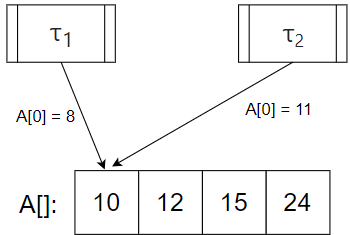
\includegraphics[width=0.4\textwidth]{images/shared_memory.png}
    \caption{An example of two processes writing to a shared in-memory array}
    \label{fig:shared_memory}
\end{figure}
\par
Elixir instead uses a message-passing model for IPC. More specifically, Elixir uses an actor-based model, where each process (actor) has its state and a message box to receive messages from other actors. Actors are responsible for sending a finite number of messages to other actors, spawning new actors and changing their behaviour based on the handling of messages received in the mailbox. Figure \ref{fig:actor_model} shows an example of how actors behave. The mailbox is not necessarily first in, first out (FIFO) but often implementations tend to be.
\begin{figure}[H]
    \centering
    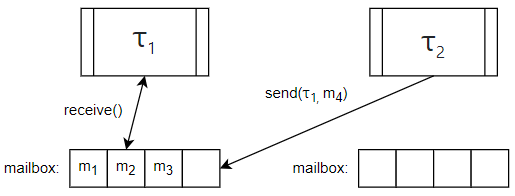
\includegraphics[width=0.6\textwidth]{images/actor_model.png}
    \caption{An example of actors sending and receiving messages under the actor model}
    \label{fig:actor_model}
\end{figure}
\par
In Elixir, a receive statement is used to read messages in the mailbox. The receive block looks through the mailbox for a message that matches a given pattern, if no messages match a given pattern, the process will block until one does.
\begin{lstlisting}[language=Elixir, xleftmargin=.4\linewidth, caption={An example of spawn/1 and spawn/4 in Elixir for spawning a new lightweight process and a new Elixir node}]
    # Example send in Elixir
    send self(), {:hello, "world"}

    # Example receive block in Elixir
    receive do
        {:hello, msg} -> IO.puts msg
    end
\end{lstlisting}
\subsection[]{Quote and Unquote}
The quote and unquote constructs in Elixir give us a deeper insight into how the programming language is implemented. Elixir is fundamentally made of tuples with three elements consisting of an atom\footnote{In Elixir, atoms are named constants, whose values are their own name. They can be identified by a preceding colon, for example, \texttt{:hello}.} that identifies the tuple, an array of metadata and finally the data. For example, the function call \texttt{sum(1, 2)} would be represented by the tuple \texttt{(:sum, [], [1, 2])} and similarly, the variable \texttt{total} would be represented by the tuple \texttt{(:total, [], Elixir)}. Using these building blocks, Elixir can begin to build what is known as a quoted expression, which is a nesting of tuples in a tree-like structure. In many other programming languages, this tree-like structure is referred to as an abstract syntax tree (AST).
\par
The quote and unquote constructs allow us to transition between Elixir syntax and quoted expressions. Using the \texttt{quote/2}\footnote{In Elixir, it is common to name functions or macros alongside their number of arguments. The function \texttt{spawn/1} refers to the function spawn, with 1 argument.} macro on an Elixir block, such as \texttt{quote do: sum(1, 2)} will return the quoted expression representing the block, in this case, \texttt{(:sum, [], [1, 2])}. Similarly, the \texttt{unquote/1} macro can be used within a quoted expression to inject code directly into the underlying expression. Figure \ref{fig:quote_unquote} shows a small example of how unquote can be applied within a quoted expression to inject a variable.
\begin{lstlisting}[language=Elixir, xleftmargin=.4\linewidth, caption={Elixir example of \texttt{quote/2} and \texttt{unquote/1}.}, label={fig:quote_unquote}]
    x = 2
    quote do: sum(1, unquote(x))
\end{lstlisting}
\par

\subsection[]{Metaprogramming}
Metaprogramming is a technique that allows developers to write a program that outputs another program. It means a program can be designed to read or transform other programs. In Elixir, metaprogramming is often used to extend the language by directly modifying the generated quoted expressions by a program. This is achieved through the quote and unquote constructs alongside macros. Macros allow for transforming code and expanding a module.
\par
In Elixir, \texttt{defmacro/2} is used to define new macros, which itself is a macro. Macros receive quoted expressions as arguments and typically inject these expressions into code before returning another quoted expression. Listing \ref{fig:unless} introduces how \texttt{defmacro/2} can be used to define the \texttt{unless/2} macro used in the standard library. Unless is the opposite of an \texttt{if/2} statement, it will execute an expression if a conditional check evaluates to false.
\begin{lstlisting}[language=Elixir, xleftmargin=.3\linewidth, caption={Elixir example of the \texttt{unless/2} macro as defined in the standard library \cite{defmacro}}., label={fig:unless}]
defmacro unless(clause, do: expression) do
  quote do
    if(!unquote(clause), do: unquote(expression))
  end
end
\end{lstlisting}
\par
Macros are both lexical and explicit. That means it is impossible to inject macros globally and it is impossible to run macros without explicit invocation. By leveraging the use of functions, quoted expressions and macros, we can begin to develop a domain-specific language (DSL). For example, constructing a DSL that overrides the standard implementations for many Elixir constructs in a style that makes verifying the correctness of Elixir programs more trivial. By default, Elixir is very difficult to verify. Elixir provides an ExUnit module, with an \texttt{assert/1} macro which could be used for loop invariants, preconditions and postconditions but doesn't support an approach that favours writing verification-aware code. As many Elixir programs are concurrent, and as Elixir uses the actor model, verifying an arbitrary Elixir program that has not been restricted or extended using macros is a challenge.
\par
Another useful feature often associated with the development of DSLs in Elixir is attributes. Attributes can be used to store additional information, as a temporary storage. Attributes also work as constants, or simply to annotate code which can be useful for other developers or the virtual machine. Listing \ref{fig:attributes} shows a basic example of annotating a function with an attribute.
\begin{lstlisting}[language=Elixir, xleftmargin=.3\linewidth, caption={Example use of attributes in Elixir}., label={fig:attributes}]
    @doc "Calculate the sum of two numbers, x and y"
    def sum(x, y) do
        x + y
    end
\end{lstlisting}

\section[]{Existing Work}
\subsection[]{Lean}
\subsection[]{C Wolf}
\subsection[]{Boogie}
\subsection[]{Dafny}
\subsection[]{Promela}
\subsection[]{Gomela}
\section[]{Modelling Elixir Programs in Promela}
\subsection[]{Basic Deadlock}
\subsection[]{Dining Philosophers}
\subsection[]{Preconditions and Postconditions}


\chapter{Promela and Elixir} \label{chap:promela_elixir}
In chapter \ref{chap:verlixir}, we will introduce the Verlixir tool. Verlixir involves the parsing of Elixir programs, which are translated into a formal model. This model is written in Process Meta Language (Promela). This chapter will introduce both Promela and Elixir. We will go through the core concepts and syntactic elements that Verlixir relies upon to provide a verification-aware Elixir. 
\section{Promela} \label{sec:promela}
Promela is the verification modelling language used by the Spin model checker, to specify concurrent processes modelling distributed systems \cite{spin}. This section will discuss some of the core features that allow systems to be modelled and verified with Spin. This section aims to give an overview of the syntax and control of Promela, so any specifications in later sections or the code artifact can be read.
\subsection{Types and Variables}
Promela is statically typed. Variables can be declared once within the current scope and then re-assigned throughout. Variables can be declared locally within the context of a process, or in the global scope, where memory is shared. The types available in Promela, and assignment to variables of these types is similar to many imperative programming languages. Promela supports the types bit, bool, byte, pid, short, int and unsigned. Variable declaration and assignment then naturally follows.
\[
\begin{aligned}
\text{int a} = 2;
\end{aligned}
\]
Promela supports \textbf{arrays}. Arrays are typed and declared with a fixed size. Array bounds are constant, so the size cannot change. Only single dimensional arrays are supported. The syntax for declaring an array is as follows.
\[
\begin{aligned}
\text{int array[10];}
\end{aligned}
\]
We can also extend the basic types using \texttt{typedef}. This allows us to define records of multiple nested types. We use these records to build a Promela library, to support model checking Elixir programs, using \textbf{embedded C} code and Promela \textbf{inlines}. Embedded C code cannot be model checked, but Promela inlines can be. These features allow us to extend Promela, and avoid some of the limitations discussed in section \ref{sec:promela_limitations} 
\subsection{Control Flow}
Promela supports some basic control flow concepts. Firstly, the \texttt{skip} expression can be used with no effect when executed, other than possibly changing the control of an executing process. The selection construct \texttt{if} can be used to evaluate expressions and execute sequences based on the evaluation of these expressions. The syntax of an if statement is unique in comparison to a typical programming language.
\begin{lstlisting}[language=promela, xleftmargin=.3\linewidth]
if
    :: 1 + 1 < 3 ->
        printf("Condition 1...");
    :: else -> 
        printf("No conditions matched");
fi
\end{lstlisting}
In Promela, $else$ is a reserved keyword that can be used in any condition. An $else$ condition will negate all the previous conditions.
Repetition can be achieved either through the \texttt{do} construct, through the use of labels or with \texttt{for} loops. We will primarily focus on \texttt{do}, as it is the most suitable for our modelling needs.
\begin{lstlisting}[language=promela, xleftmargin=.3\linewidth]
do
    :: a < 10 -> 
        a = a + 1;
    :: a < 10 ->
        a = a + 2;
    :: else -> 
        break;
od
\end{lstlisting}
Unlike \texttt{if}, which selects sequentially, \texttt{do} will non-deterministically select a true branch to execute. This means for the above example, for a given execution, we cannot say how many iterations are performed. The \texttt{break} keyword is reserved for explicitly breaking out of the loop.
\\ \\
An important concept in contract specification is the \textbf{assert} keyword. An assertion is a logical statement that is expected to be true at a given point in the program. If an assertion is false, a violation is reported.
\subsection{Processes}
An imperative component of understanding the power of the Spin model checker is understanding how processes can run concurrently. Every Promela model requires an initial process that is spawned in the initial system state and determines the control of the program from the initial state. The \texttt{init} keyword is reserved for this purpose. Other processes can be defined using the \texttt{proctype} keyword and then spawned with \texttt{run}. Each process is assigned a process id (pid) which can be accessed within the context of a process using globally defined read-only variable \texttt{\_pid}. We can now define two processes, a process active in the initial state and a second process that is spawned.
\begin{lstlisting}[language=promela, xleftmargin=.3\linewidth, caption={Defining and spawning processes in Promela}., label={fig:promela_processes}]
    proctype SomeProcess(int a) {
        printf("Do something with %d\n", a);
    }
    
    init {
        int p1;
        p1 = run SomeProcess(10);

        printf("Init process spawned at %d\n", _pid);
        printf("Process 1 spawned at %d\n", p1);
    }
\end{lstlisting}
Processes run independently of one another, so a parent process terminating will not necessarily result in the termination of a child. Spin sets a limit of 255 concurrently executing processes. Multiple processes can be spawned in a single transition by using the \textbf{atomic} construct, which will ensure that no spawning process is scheduled, until all atomic processes have been scheduled. Similarly to atomicity, \texttt{d\_step} can be used to enforce multiple statements are treated as a single indivisible step. Unlike \texttt{atomic}, \texttt{d\_step} cannot block or jump.
\\ \\
Instead of \texttt{init}, we could have used an \textbf{active proctype}. Every \textbf{active proctype} is spawned in the initial state, allowing for more than one process to initially run.
\subsection{Channels}
The final concept to briefly discuss, is the asynchronous communication primitive, channels. Promela allows channels to be specified using the predefined data type \texttt{chan}. To correctly specify communication, we often need to allow messages of multiple types to be written to channels. For this reason, Promela introduces \texttt{mtype} that allows for the introduction of symbolic names for constant values.
\[
\text{mtype = \{ BROADCAST \};}
\]
Now, we can define a channel that expects a message to contain multiple fields and is bound to contain a maximum of 10 messages at any time.
\[
\text{chan global\_broadcast = [10] of \{ mtype, int \};}
\]
We now input messages to the channel using the (!) operator.
\[
\text{global\_broadcast ! BROADCAST, 1;}
\]
Similarly, we read messages from the channel in a first-in, first-out (FIFO) order.
\[
\begin{aligned}
& \text{int x;} \\
& \text{global\_broadcast ? BROADCAST, x;}
\end{aligned}
\]
Where the variable $x$ stores the resulting \texttt{int}, assuming the first message in the channel is of type \texttt{BROADCAST}. Sending and receiving from channels also supports an alternative flavour. The (!!) and (??) operators are used for sorted insertion and random selection. \textbf{Sorted insertion} (!!), will insert a message into the channel in a sorted order, based on the first field of the message. \textbf{Random receive} (??), is not random. As opposed to FIFO, it will select the first message in the channel that matches a given pattern. We call this first-in, first-fireable-out (FIFFO).
\subsection{Promela Example}
We will now provide a simple example of a Promela specification. The specification models Dijkstra's Semaphore. It consists of two labelled processes, and an initial process to coordinate the system. A shared channel is used, with a buffer size of 0, which means the channel is blocking (rendezvous). Listing \ref{lst:dijkstra_semaphore} shows the Promela specification.
\begin{lstlisting}[language=promela, xleftmargin=.3\linewidth, caption={Dijkstra's Semaphore in Promela}, label={lst:dijkstra_semaphore}]
#define p	0
#define v	1

chan sema = [0] of { bit };

proctype dijkstra() {	
    byte count = 1;

    do
    :: (count == 1) ->
        sema!p; count = 0
    :: (count == 0) ->
        sema?v; count = 1
    od	
}

proctype user() {	
    do
    :: sema?p;
        /* critical section */
    sema!v;
        /* non-critical section */
    od
}

init {	
    run dijkstra();
    run user();
    run user();
    run user()
}
\end{lstlisting}
The semaphore guarantees that only one of the user processes can enter its critical section at a time.
\subsection{Limitations} \label{sec:promela_limitations}
Promela is a powerful language for modelling concurrent systems, but it has limitations for capturing the full complexity of a real-world system. In general, hand-translations of a system into Promela can avoid some of these limitations with careful design. However, we are approaching this limits from an Elixir perspective, where features of Elixir may not be easily translated into Promela.
\begin{itemize}
    \item \textbf{Compute}: Promela is not designed to model complex computations. It does not support floating-point arithmetic, so we are limited to working with integers.
    \item \textbf{Memory}: Promela does not support dynamic memory allocation. This means we cannot model systems that require dynamic memory allocation, for example, linked lists.
    \item \textbf{Functions}: Promela does not support functions. It has no notion of a function call or return. By extension, Promela does not support recursion.
    \item \textbf{Randomness}: a Spin execution may not be deterministic, but it cannot model true randomness.
    \item \textbf{Probability}: there is no mechanism for modelling probabilistic behaviour, all correctness claims are checked unconditionally.
    \item \textbf{Time}: there is no notion of a system block, or related time properties in Promela. This means we cannot model sleeping threads.
\end{itemize}
In chapter \ref{chap:design}, we will discuss how we can overcome some of these limitations. In particular, how we overcome the lack of functions and dynamic memory, by introducing a Promela library, which handles these features.
\subsection{Summary}
This basic introduction to the syntax of the Promela modelling language, aims to make the reader familiar with the syntax involved in writing Promela specifications. It is not an exhaustive guide but should form a basis for understanding specifications present in a later section or the code artifact.

\section{Elixir}
Elixir is a dynamic, functional language for building scalable and maintainable applications \cite{elixir}. Elixir programs run on the BEAM virtual machine \cite{beam}, which is also used to run the Erlang programming language \cite{erlang}. Elixir was designed by José Valim and first released in 2012. Elixir is built on top of Erlang and hence inherits many of the abstractions designed for building distributed systems. This section aims to give a brief overview of Elixir, it is not a complete guide but rather aims to give non-Elixir programmers a basic understanding of the language.
\\ \\
BEAM is a virtual machine that executes user programs in the Erlang Runtime System (ERTS). BEAM is a register machine where all instructions operate on named registers containing Erlang terms such as integers or tuples.
\\ \\
We have recently seen companies adopting Elixir in industry, in particular in domains such as telecoms and instant messaging. The Phoenix Framework \cite{phoenix} is a framework for building interactive web applications natively in Elixir, that can take advantage of Elixir's multi-processing and fault tolerance to build scalable web applications. The audio and video communication application Discord \cite{discord} uses Elixir to manage its 11 million concurrent users and the Financial Times \cite{ft} have begun migrating from Java to Elixir to enjoy the much smaller memory usage by comparison.
\\ \\
Elixir supports multi-processing in two key ways: nodes and processes. Each node is an instance of BEAM (a single operating system process), when an Elixir program is executed, a new instance of BEAM is instantiated for it to run on. In contrast, an Elixir process is not an operating system process. An Elixir process is lightweight in terms of memory and CPU usage (even in comparison to threads that many other programming languages favour). Elixir processes can run concurrently with one another and are completely isolated from one another. Elixir processes communicate via message passing.
\begin{lstlisting}[language=Elixir, xleftmargin=.2\linewidth, caption={An example of spawn/1 and spawn/4 in Elixir for spawning a new lightweight process and a new Elixir node}]
    # Spawn a new process
    spawn(fn -> 1 + 2 end)

    # Create a new BEAM instance
    Node.spawn(:"node1@localhost", MyModule, :start, [])
\end{lstlisting}

In Elixir, a receive statement is used to read messages in the mailbox. The receive block looks through the mailbox for a message that matches a given pattern. If no messages match the pattern, the process will block until one does.
\begin{lstlisting}[language=Elixir, xleftmargin=.4\linewidth, caption={An example of spawn/1 and spawn/4 in Elixir for spawning a new lightweight process and a new Elixir node}]
    # Example send in Elixir
    send self(), {:hello, "world"}

    # Example receive block in Elixir
    receive do
        {:hello, msg} -> IO.puts msg
    end
\end{lstlisting}
\subsection{Verifiable Feature Set} \label{sec:verifiable_feature_set}
In chapter \ref{chap:verlixir}, we will introduce Verlixir. Verlixir is designed to support a reduced set of core Elixir constructs. We will introduce these constructs here to give an overview of what the tool is capable of supporting.
\\ \\
Everything in Elixir is an expression. This means that every piece of code returns a value. For example, an $if$ statement will return a value dependent on the branch taken. This means that any expression can be matched on, using Elixir's match (=) operator. We can use pattern matching to match on the shape of an expression's evaluation. The set of expressions supported by Verlixir are:
\begin{itemize}
    \item \textbf{Values}: any value of a basic, primitive type such as integers and booleans. Elixir also has a concept of $atoms$. An atom is identified by a preceding colon (:), and is followed by letters, digits, `\_', `@' or a string.
    \item \textbf{Variables}: Elixir is dynamically, strongly typed. Variables are bound to using the match operator. Variable names start with lowercase letters. The `\_' character can be used to match an expression of any shape.
    \item \textbf{Data structures}: structures such as lists and tuples are treated as values. Lists are dynamic, whereas tuples are fixed in size. Lists are written as [1, 2, 3] and tuples are written as \{1, 2, 3\}. We can match on the shape of these data structures using pattern matching.
    \item \textbf{Pattern matching}: pattern matching can be used to match on the shape of an expression. In the context of a conditional guard, values can be used to evaluate the shape of an expression, where as variables can be used to bind to the value of an expression. For example, the pattern ${:ok, value}$, can be used to assign to the variable $value$ if the expression is a tuple shape, with an atom $ok$ as the first element.
    \item \textbf{Functions}: functions are defined using the $def$ keyword. Functions can group multiple sequentially executable expressions. Any function can be called or spawned as a new process or node.
    \item \textbf{Modules}: functions are grouped into modules.
    \item \textbf{Message passing}: Elixir's actor model supports message passing. Messages are sent and received between actors and their mailboxes.
    \item \textbf{Control flow structures}: Elixir supports many control flow expressions. For example, $if$, $case$, $unless$ and $for$. All of these introduce a new scope. They are expressions and can be matched on.
\end{itemize}
The feature set supported has been shown expressive enough to support real-world systems in chapter \ref{chap:eval}. We omit some features of Elixir. For example, data structures like sets and maps are not supported. We determined lists sufficient for our purposes. The supported feature set can be easily extended to support other data structures.
\subsection{Type Specifications}
Type specifications are imperative for the correctness of Verlixir specifications. Verlixir supports some basic types such as \texttt{integer()}, \texttt{boolean()}, \texttt{atom()} and \texttt{pid()}. 
\\ \\
In type specifications, message types are typed as \texttt{atom()}. The atom \texttt{:ok} is reserved to identify a \textbf{non-returning function}. In Elixir, all functions return a value, so in this context, a `non-returning function', is a function that's value is never matched. We briefly demonstrate the type specifications for two functions, the first, is a non-returning function with no arguments and the second function, takes two arguments and returns an integer.
\begin{lstlisting}[language=Elixir, xleftmargin=.3\linewidth, caption={Valid type specification examples}.]
    (*@\fbox{@spec bind\_server() :: :ok}@*)
    def bind_server do
        ...
    end

    (*@\fbox{@spec add(integer(), integer()) :: integer()}@*)
    def add a, b do
        ...
    end
\end{lstlisting}
Notice ($::$) marks the return type of the function. If these values are matched in the function body, they should not be matched to a different type.
\\ \\
Within a correct Verlixir specification, any message should also be typed. To ensure this, any instance of a message should begin with an atom which we will refer to as the \textbf{message type}. For example, \texttt{\{:bind\}} and \texttt{\{:calculate, 10, 20\}} are valid specification messages. The message, \texttt{\{false, 15\}}, would be ignored by Verlixir, as it does not begin with an atom. 
\subsection{Summary}
In this chapter, we learned about Elixir, the programming language built on top of Erlang and we explored some basic approaches to designing concurrent systems with it. The next section will explore how these core tools can be used in tandem, to provide developers guarantees over large-scale, distributed Elixir-based systems.
\chapter{Veriflixir}
Veriflixir is the main project contribution. The Veriflixir toolchain supports the simulation and verification of a set of Elixir programs. This set is named LTLixir and is detailed in section \ref{sec:ltlixir}. This chapter aims to inform the reader of the constructs defined in LTLixir and how Veriflixir can be used to reason about them. \ref{sec:ltlixir} introduces the LTLixir language and its constructs. \ref{sec:verifiable} provides an example of specifying a verifiable system and how Veriflixir can be used to detect violations of a specification. The subsequent subsections provide further details of more interesting features of LTLixir, such as specifying temporal properties.
\section{LTLixir} \label{sec:ltlixir}
LTLixir is the multi-purpose specification language that compiles to BEAM byte-code and is supported for verification by Veriflixir. Primarily, LTLixir is a subset of Elixir supporting both sequential and concurrent execution. This subset is expressive enough to well-known distributed algorithms such as basic paxos \cite{basic-paxos} and the alternating-bit protocol \cite{ab-protocol}. LTLixir extends Elixir with constructs for specifying temporal properties, specifically LTL properties (where LTLixir derives its name) as well as Floyd-Hoare style logic for specifying pre- and post-conditions. Specifications can be parameterized to identify violations of properties on specific configurations. 
\par

\section{Constructing a Verifiable Elixir Program} \label{sec:verifiable}
This section will walk through the basic construction of an LTLixir program, and show how we can verify the properties of the program using Veriflixir. To begin, we define a server and client process. The server is responsible for creating clients and communicating with them. 
\begin{lstlisting}[language=Elixir, xleftmargin=.3\linewidth, caption={Elixir definition for a server and client module}., label={fig:basic_server}]
    defmodule Server do
        def start_server do
            client = spawn(Client, :start_client, [])
        end
    end

    defmodule Client do
        def start_client do
            IO.puts "Client booted"
        end
    end
\end{lstlisting}
To begin, the server spawns a single client process, which writes to stdio. To ensure correctness when verifying properties of the system, we remove ambiguity by being particular in our naming of the functions \texttt{start\_server} and \texttt{start\_client}. Notice we could name both functions \texttt{start}, but this ambiguity can make it more difficult to digest a trail produced by Veriflixir. With the system implemented, we must now declare an entry point to the system that Veriflixir will use to begin verification. For this example, we can define \texttt{Server.server\_start} as the entry point using an attribute \texttt{\@vae\_init}.

\begin{lstlisting}[language=Elixir, xleftmargin=.3\linewidth, caption={Declaring an entry point to the system}., label={fig:vae_init}]
    @vae_init true
    def start_server do
        client = spawn(Client, :start_client, [])
    end
\end{lstlisting}
Although we set the attribute \texttt{vae\_init} to \texttt{true}, note it is not required that other functions are set to \texttt{false}, this is already implied. With an entry point specified, we can begin using the available tools. By default, Veriflixir reports the presence deadlocks and livelocks in the system. When specifying systems in LTLixir, we do not lose the capability to compile our program to BEAM byte-code, hence the system can still run as a regular Elixir program. For example, using mix \cite{mix}.
\begin{lstlisting}[language=bash, xleftmargin=.3\linewidth]
    $ mix run -e Server.start_server
    Generated app
    Client booted
\end{lstlisting}
More interestingly, we can now use Veriflixir before the Erlang Run-Time System (ERTS) to verify the system adheres to our specification. With no additional properties defined, by running Veriflixir we are ensuring that every possible execution results in a program termination. The presence of a deadlock or livelock will be reported. We can run the Veriflixir executable by passing optional arguments as the path to the specification file. For example, we use the simulator flag $-s$ to run a single simulation of the system.
\begin{lstlisting}[language=bash, xleftmargin=.3\linewidth]
    $ ./veriflixir -s basic_example.ex 
    Client booted
\end{lstlisting}
Alternatively, we can use the $-v$ flag to run the verifier on the specification.
\begin{lstlisting}[language=bash, xleftmargin=.3\linewidth]
    $ ./veriflixir -v basic_example.ex 
    Model checking ran successfully. 0 error(s) found.
    The verifier terminated with no errors.
\end{lstlisting}
\subsection{Detecting a Deadlock} \label{sec:deadlock}
Now we have a basic understanding of what is required to write a specification, we will use Veriflixir to detect a deadlock in the system. By default, the verifier will detect the presence of deadlocks and livelocks in the system. Deadlocks in Elixir programs can be introduced by circular waits, where two simultaneously executing processes are both waiting for a message from the other. To demonstrate this, we modify the existing client and server by introducing a circular wait. The server will now spawn the process, and expect to receive a message from the client, meanwhile, the client will expect to receive a message from the server. The resulting server and client processes are modeled below.
\begin{lstlisting}[language=Elixir, xleftmargin=.3\linewidth, caption={A simple Elixir system with a deadlock}.]
    defmodule Server do
    @vae_init true
    def start_server do
      client = spawn(Client, :start_client, [])
      receive do
        {:im_alive} -> IO.puts "Client is alive"
      end
    end
  end
  
  defmodule Client do
    def start_client do
      receive do
        {:binding} -> IO.puts "Client bound"
      end
    end
  end  
\end{lstlisting}
In this simple example, any execution of the system will result in a deadlock, the system can be considered deterministic in this regard. In many real-world systems with multiple processes, the presence of a deadlock can be difficult to detect due to multiple interleavings. Let's take another look at what happens when we execute the program, run a simulation and run the verifier.
\begin{lstlisting}[language=bash, xleftmargin=.3\linewidth]
$ mix run -e Server.start_server
Generated app
Client booted

\end{lstlisting}
Notice when running the Elixir program, nothing is output to stdio, even though a naive Elixir programmer could think one of the two \texttt{IO.puts} statements is executed. Of course, we know this not to be the case but let's compare the outputs from running Veriflixir.
\begin{lstlisting}[language=bash, xleftmargin=.3\linewidth]
    $ ./veriflixir -s basic_example.ex
    timeout
\end{lstlisting}
The simulator terminates, reporting a timeout. Already, running our specification using Veriflixir provides more information than running the Elixir program. Let's now run the verifier.
\begin{lstlisting}[language=bash, xleftmargin=.2\linewidth]
    $ ./veriflixir -v basic_example.ex
    Model checking ran successfully. 1 error(s) found.
    The program likely reached a deadlock. Generating trace.
    [8] (proc_0) init:4 [receive do]
    [9] (proc_0) init:4 [receive do]
    [10] (proc_0) init:5 [{:im_alive} -> IO.puts "Client is alive"]
    [13] (proc_1) start_client:13 [{:binding} -> IO.puts "Client bound"]
    <<< END OF TRAIL, FINAL STATES: >>>
    [14] (proc_1) start_client:13 [{:binding} -> IO.puts "Client bound"]
    [15] (proc_0) init:5 [{:im_alive} -> IO.puts "Client is alive"]
\end{lstlisting}
Running the verifier produces much more output. Let's break down step by step the output produced by Veriflixir. The first line of the output informs us that the verifier successfully terminated on the input, along with how many errors were found. If an error is found, Veriflixir will use heuristics to profile the type of error, in this case, it has determined the program likely deadlocked. Once determining the error type, an error trail is produced to debug the source of the error. The underlying model derived from the LTLixir specification does not have a one-to-one mapping to the original Elixir code, hence again heuristics are applied to determine where in the Elixir program the trail is produced from. In this case, we can see reference to \texttt{init}, the entry point to the system (annotated previously by \texttt{@vae\_init}). Alongside the process, we can see a line number referring to a line number in the Elixir file, as well as the line of code the line refers to. With the exception of the system entry point, all other function names are labeled as in the original program, for example, $start\_client$. The remaining information on a trail line is less relevant to most users. The first number on a line is the step number (some of these may be omitted for simplicity). The \texttt{proc\_n} refers both to process numbers and function call stack depth.
\par
Now we understand how to read a single line of the trail, we can read the trail in sequential order to learn the interleaving that resulted in the error. In this instance, we can see the server reaches line 5 where it waits for an \texttt{:im\_alive} message from the client and similarly, the client is waiting for a \texttt{:binding} message.
\subsection{Linear Temporal Logic}
We now introduce Linear-time Temporal Logic to our systems to allow us to write more interesting LTLixir specifications. Before doing so, we must detour to type specifications. Type specifications had been previously omitted from examples, but they are imperative for the correctness of LTLixir specifications. LTLixir supports some basic types such as \texttt{integer()}, \texttt{boolean()}, \texttt{atom()} and \texttt{pid()}. Internally, Veriflixir treats process identifiers as integers, so \texttt{integer()} and \texttt{pid()} can be used interchangeably in specifications, for the following examples, we refer to process identifiers as integers. Message passing in specifications should be typed using atoms. To ensure this, any instance of a message should begin with an atom (which we will refer to as the message type). For example, \texttt{{:bind}} and \texttt{{:calculate, 10, 20}} are valid specification messages, \texttt{{false}} would be ignored by Veriflixir. In type specifications, message types are typed as \texttt{atom()}. The atom \texttt{:ok} is reserved to identify non-returning functions. In Elixir, all functions return a value, so in this context, a 'non-returning function' is a function that's value is never matched. We briefly demonstrate the type specifications for two functions, the first is a non-returning function with no arguments and the second function takes two arguments and returns an integer.
\begin{lstlisting}[language=Elixir, xleftmargin=.3\linewidth, caption={Valid type specification examples}.]
    @spec start_server() :: :ok
    def start_server do
        ...
    end

    @spec add(integer(), integer()) :: integer()
    def add a, b do
        ...
    end
\end{lstlisting}
Notice $::$ marks the return type of the function. If these values are matched in the function body, they should not be matched to a different type.
\par
Let's now re-design the server and client processes so we can introduce temporal properties to reason about. The server will now spawn $n$ clients, bind the clients to itself and then await a response from all three clients. To achieve this, we introduce two variables \texttt{client\_n} and \texttt{alive\_clients} that will later be used in our temporal specification.
\begin{lstlisting}[language=Elixir, xleftmargin=.2\linewidth]
    def start_server do
        client_n = 3
        alive_clients = 0
        for _ <- 1..client_n do
            client = spawn(Client, :start_client, [])
            send(client, {:bind, self()})
        end
        alive_clients = check_clients(client_n, alive_clients)
    end
\end{lstlisting}
The implementation of the client process and the \texttt{check\_clients/2} function have been redacted, without understanding their implementation, we can still use our specification to verify the system acts as intended. We introduce our first LTL formula, which verifies that eventually, the number of alive clients is equal to $n$. To introduce an LTL formula, we can use the \texttt{@ltl} attribute. The attribute assigns an LTL formula, as a string, to function. The LTL grammar is defined as the following.
\begin{bnf*}
    \bnfprod{ltl}
      {\bnfpn{operand} \bnfor ( \bnfpn{ltl} ) \bnfor \bnfpn{ltl} \bnfpn{binop} \bnfpn{ltl} \bnfor \bnfpn{unop} \bnfpn{ltl}}\\
    \bnfprod{operand}
      {true \bnfor false \bnfor var \bnfor int \bnfor elixir\_expr}\\
    \bnfprod{unop}
      {\square \bnfor \lozenge \bnfor !}\\
    \bnfprod{binop}
      {U \bnfor W \bnfor V \bnfor \&\& \bnfor || \bnfor \rightarrow \bnfor \leftrightarrow }\\
\end{bnf*}
We want to verify that eventually, the number of alive clients equals the number the server created, we can write this using the formula $\lozenge (alive\_clients \equiv client\_n)$. Using the LTL attribute, we can update our server process.
\begin{lstlisting}[language=Elixir, xleftmargin=.3\linewidth, caption={Example LTL property}.]
    @vae_init true
    @spec start_server() :: :ok
    @ltl "<>(alive_clients == client_n)"
    def start_server do
        ...
    end
\end{lstlisting}
The entire program can be found in appendix \ref{appendix:ex4}. Let us run Veriflixir on the system.
\begin{lstlisting}[language=bash, xleftmargin=.3\linewidth]
    $ ./veriflixir -v basic_example.ex
    Model checking ran successfully. 0 error(s) found.
    The verifier terminated with no errors.
\end{lstlisting}
Let's update the LTL formula, by replacing \texttt{clients\_n} with the number 1 ($\lozenge (alive\_clients \equiv 1)$). We run the verifier again.
\begin{lstlisting}[language=bash, xleftmargin=.1\linewidth]
    $ ./veriflixir -v basic_example.ex
    Model checking ran successfully. 1 error(s) found.
    The program is livelocked, or an ltl property was violated. Generating trace.
\end{lstlisting}
The examples show how LTL properties can be specified and used to verify the system. Given the first LTL property was accepted, we know the formula holds. This is likely because the implementations of the client and \texttt{check\_clients/2} are correct, but we should also specify properties to check the validity of these functions instead of making this assumption.
\par
To help with readability, we can define inline predicates to use in LTL formulae. The predicates that can be defined are formed from a subset of the LTL grammar without the temporal modalities. Inline predicates can refer to variables in the scope of the function. For example, we can define a predicate \( p \) as $alive\_clients \equiv client\_n$. The predicates can take the name of any variable but should not reference variables that are already in scope. To help construct our example, let's also define a predicate \( q \) and set it to \( \neg p \). Using these predicates, we can strengthen our LTL formula to \( (q) \mathcal{U} (\square p) \). Informally, this formula states that there is a moment in time where $alive\_clients \equiv client\_n$, and from that moment onwards this property holds until termination. We can update our \texttt{start\_server} function to reflect this.
\begin{lstlisting}[language=Elixir, xleftmargin=.3\linewidth]
    @ltl "(q)U([]p)"
    def start_server do
      client_n = 3
      alive_clients = 0
      predicate p, alive_clients == client_n
      predicate q, !p
      ...
    end
\end{lstlisting}
\subsection{Pre- and Post-Conditions}
Veriflixir has been designed to target system designs that are bounded in execution. As many real-world systems run long-lived processes, it is important that when writing LTLixir specifications there is a focus on termination conditions. For many distributed algorithms this could be completing a round of communication, reaching a consensus, awaiting a specific message to be received or reaching a stable system state. To aid this, LTLixir supports Floyd-Hoare style pre- and post-conditions in function definitions. These are particularly useful for ensuring proper bounds on the system that help define correct execution. Consider a process that should send and receive a single message each round. We can define a pre-condition on a bounded parameter to ensure the process does not run indefinitely. Let us refactor the client process to complete a number of rounds (determined by the server) before terminating. The client will receive a \texttt{:bind} message from the server, deciding how many rounds to complete and then will recurse until it has completed all the rounds.
\begin{lstlisting}[language=Elixir, xleftmargin=.3\linewidth]
    defmodule Client do
        @spec start_client() :: :ok
        def start_client do
            {server, rounds} = receive do
            {:bind, sender, round_limit} -> {sender, round_limit}
            end
            next_round(server, rounds)
        end

        @spec next_round(pid(), integer()) :: :ok
        def next_round(server, rounds) do
            send(server, {:im_alive})
            next_round(server, rounds - 1)
        end
    end
\end{lstlisting}
We can again run this with mix, and we can observe that the server terminates. Although our clients did not terminate, there was no indication of this. Processes in Elixir are isolated, so the termination of the server does not imply the termination of the clients (links can resolve this \cite{elixir_links}). It has become challenging to determine if our client is truely behaving as intended.
\begin{lstlisting}[language=bash, xleftmargin=.3\linewidth]
    $ mix run -e Server.start_server
    Generated app
    $
\end{lstlisting}
To help reason about this, we introduce the \texttt{defv} macro from the LTLixir specification language. The \texttt{defv} macro is used to define pre- and post-conditions on functions. Pre-conditions check conditions regarding the values of function arguments on entry to the function and similarly, post-conditions can assert conditions on values within the scope of the function on exit. For example, we could define a function \texttt{add\_positives/2} that takes two strictly positive numbers and sums them.
\begin{lstlisting}[language=Elixir, xleftmargin=.0\linewidth, caption={Example usage of pre- and post-conditions in LTLixir}]
    defv add_positives(a, b), pre: a > 0 and b > 0, post: result == a + b do
        ...
    end
\end{lstlisting}
With this definition, we gain assurances that the implementation of the function behaves as we expect and that no other function interacts with the function in a manner that violates our expected behavior. Let's take a similar approach with our client to help understand why the program does not terminate.
\begin{lstlisting}[language=Elixir, xleftmargin=.3\linewidth]
    @spec next_round(pid(), integer()) :: :ok
    defv next_round(server, rounds), pre: rounds >= 0 do
        ...
    end
\end{lstlisting}
We can run Veriflixir on the system to verify the pre-condition holds for every possible execution.
\begin{lstlisting}[language=bash, xleftmargin=.1\linewidth]
    $ ./veriflixir -v basic_example.ex
    Model checking ran successfully. 1 error(s) found.
    An LTL, pre- or post-condition was violated. Generating trace.
    Violated: assertion violated (rounds>=0) (at depth 45).
\end{lstlisting}
Veriflixir reports an error, in particular, it notes the violation of an assertion. An assertion violation can be a violation of an LTL formula, and pre-condition or a post-condition. In this case, it outputs the assertion that was violated \texttt{rounds >= 0}, which we are aware is our pre-condition. The depth refers to how many transitions were taken in the execution path before violation, to most users this information is not useful.
\subsection{Parameterized Systems}
Up to this point, we have declared various system properties such as \texttt{client\_n}, \texttt{alive\_client} and \texttt{rounds}. In reality, the value assigned to these properties could be determined by many factors and it may not be known to the developer at the time of writing the specification. To support this, LTLixir allows us to declare these properties as parameters, in particular, we want to declare concurrency parameters. We define concurrency parameters are variables that impact the behaviour of a distributed system (we will simply refer to them as parameters going forward). For example, in a consensus algorithm such as paxos, we may have variables to determine the number of acceptors, proposers and size of a quorum. We can declare these variables as parameters in the specification in order to verify the system for multiple possible configurations. Typically, the values used in these auto-generated configurations will be small values as large values may lead to a state-space that becomes difficult to explore.
\par
To mark a variable as a parameter, we again make use of attributes. The \texttt{@params} attribute takes a tuple of atoms referencing variables in the function scope. For example, \texttt{@params {:x, :y}} declares that $x$ and $y$ are configurable parameters that the verifier will explore. We can apply this definition to our existing server process.
\begin{lstlisting}[language=Elixir, xleftmargin=.3\linewidth, caption={Example of declaring concurrency parameters in specification.}]
    @params {:client_n, :number_of_rounds}
    def start_server do
      client_n = 3
      number_of_rounds = 2
      predicate p, alive_clients == client_n * number_of_rounds
      ...
    end
\end{lstlisting}
We can declare as many parameters as required. The values matched in the declaration of the variables will be ignored if we run Veriflixir in parameterized mode. To run the verifier, we can use the $-p$ flag. The verifier will calculate an acceptance confidence, \(\alpha \in [0, 1]\), where an $\alpha$ of 1 indicates all configurations were accepted by the verifier and an $\alpha$ of 0 indicates no configurations were accepted. In the case $\alpha < 1$, the verifier will output configurations that lead to violations in the system. Then, the system can run in verification mode to reproduce a trail that results in the violation. To run the parameterized verification, we use the same command but with the $-p$ flag.
\begin{lstlisting}[language=bash, xleftmargin=.1\linewidth]
    $ ./veriflixir -p basic_example.ex 
    Generating models.
    Generated 9 models.
    Acceptance confidence: 1.
\end{lstlisting}
We can introduce a bug into our program that will cause a violation of the specification to show the output of the verifier under these circumstances. To introduce a bug, we are going to conditionally call \texttt{check\_clients/2} if \texttt{client\_n > 1} holds.
\begin{lstlisting}[language=Elixir, xleftmargin=.1\linewidth]
@params {:number_of_rounds}
def start_server do
    ...
    alive_clients = if number_of_rounds > 1 do
        check_clients(client_n * number_of_rounds, alive_clients)
    else
        0
    end
end
\end{lstlisting}
This will now result in cases where the temporal property is violated, as $\texttt{alive\_clients} \equiv \texttt{client\_n} * \texttt{number\_of\_rounds}$ will not hold for all configurations. Note that we have reduced the parameters down to just \texttt{\{number\_of\_rounds\}}. The system is theoretically capable of handling any number of parameters in its search, however the computational cost of exploring the state-space grows exponentially with the number of parameters, hence in reality we should use our understanding of the system to determine which parameters to test at a time.
\begin{lstlisting}[language=bash, xleftmargin=.1\linewidth]
$ ./veriflixir -p 3 basic_example.ex`
Generating models.
Generated 3 models.
Acceptance confidence: 0.6666666666666667.
Violations found in models:
Model with params: {"number_of_rounds": '1'}
Assign these parameters to the system and re-run the verifier in verification mode to gather a trace.
\end{lstlisting}
The system found a violation for the assignment of 1 to \texttt{number\_of\_rounds}. To investigate, we could run the verifier using the $-v$ flag on this configuration. We also now see our acceptance confidence has dropped below 1, due to an error produced by one of the configurations. It's also useful to note that Veriflixir was executed with $-p 3$, this sets the range of values for the parameter, large numbers are not recommended and most users will find 3 sufficient. 
\section{Summary}
We have now given a high-level overview of Veriflixir, the verification toolchain capable of verifying Elixir programs written using the LTLixir specification. We saw how to use Veriflixir to simulate executions of the system, verify our system's adherence to a specification and parameterize concurrency parameters for exploration. This chapter also exposed how to use LTLixir constructs to reason about temporal properties as well as how pre- and post-conditions can drive functional correctness. The next chapter will begin to explore the implementation behind Veriflixir.
\chapter{Design of Verlixir} \label{chap:design}
This chapter provides an in-depth insight into the design decisions that were made during the development of Verlixir and LTLixir. The chapter will begin by providing a high-level overview of where the relevant components fit into the toolchain, as well as providing an architectural overview of the tool. Section \ref{sec:specification_language} will discuss the design of LTLixir and section \ref{sec:modelling_elixir_programs} will describe the main techniques Verlixir applies in the analysis and modelling of a specification. Finally, section \ref{sec:simulation_verification} will describe how the outputs generated by Verlixir are derived.  
\section{Verlixir Toolchain} \label{sec:toolchain}
We will now introduce where the new tools fit into the grater toolchain. Figure \ref{fig:high_level} shows a high-level overview of the toolchain. Given an LTLixir specification, there are two main paths to be taken. Either, the underlying elixir program can be compiled and ran on the ERTS as normal, or the program can be modelled by Verlixir and verified with Spin.
\begin{figure}[H]
    \centering
    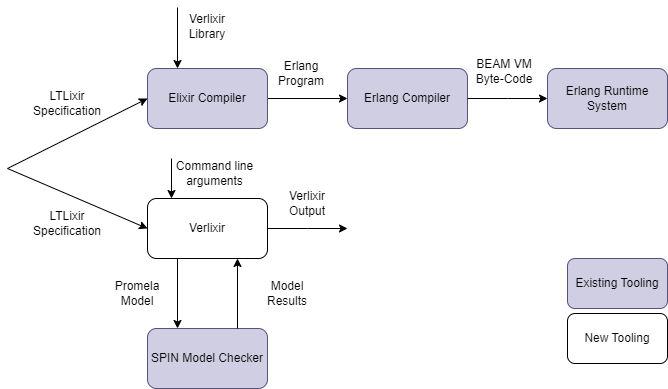
\includegraphics[width=0.9\textwidth]{images/high_level_system_v2.drawio.png}
    \caption{High-level overview of the verifiable Elixir toolchain.}
    \label{fig:high_level}
\end{figure}
Figure \ref{fig:low_level} provides an in-depth insight into the architecture underlying Verlixir.
\begin{figure}[H]
    \centering
    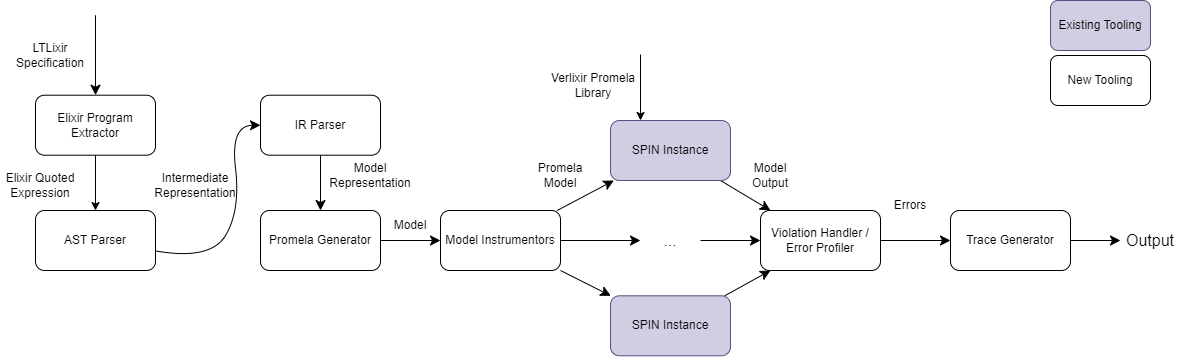
\includegraphics[width=1\textwidth]{images/detailed_diagram_v2.drawio.png}
    \caption{Verlixir design.}
    \label{fig:low_level}
\end{figure}
Before we provide an in-depth discussion on the design of Verlixir, we will summarise the components of the tool.
\begin{itemize}
    \item \textbf{LTLixir Specification}: Specification of an Elixir program to be parsed by Verlixir.
    \item \textbf{Elixir Extractor}: Converts the Elixir program into a quoted expression.
    \item \textbf{AST Parser}: Parses the quoted expression into an intermediate representation.
    \item \textbf{IR Parser}: Parses the intermediate representation, collecting relevant information for the model generator.
    \item \textbf{Promela Generator}: Writes a Promela model from the intermediate representation.
    \item \textbf{Model Instrumentors}: Instruments the model for appropriate verification (depending on system and user requirements).
    \item \textbf{Violation Handler}: Handles the output of the model checker by mapping violations back to the original Elixir program.
    \item \textbf{Trace Generator}: Generates an error trace from the mapped Elixir violations.
\end{itemize}
\section{Specification Language} \label{sec:specification_language}
LTLixir is a specification language that can be used to reason about the time and change of an Elixir system using LTL formulae. An LTLixir specification is the input to Verlixir and is used to guide the model generation process. Primarily, LTLixir supports a restricted subset of Elixir, with additional constructs to support specification properties. This section will primarily discuss the design decisions behind the additional constructs. For information on how LTLixir is transformed in model generation, see section \ref{sec:supporting_ltl}.
\\ \\
\subsubsection{Specification Constructs}
There is only one construct in LTLixir that is imperative to successfully interact with the simulator and verifier. \texttt{@init} is an attribute that is assigned a value, $v \in \{true, false\}$. The attribute, along with all the attributes we present, are ghost variables, so will not cause issues when running within the ERTS. Importantly, for Verlixir, it is used to determine an entry point to the system.
\\ \\
\subsubsection{Attributes}
All the remaining constructs of the specification are optional to the verification of the system. Similarly to the \texttt{@init} attribute, \texttt{@spec}, \texttt{@ltl} and \texttt{@model} are all attributes that are assigned values. The \texttt{@spec} is already well-defined in the Elixir language, although it is noted that type specifications do not instrument Elixir programs in any way. Instead, \texttt{@spec} can be used by analysis tools that run on Elixir programs. In our case, we reduce the possible type specifications which can be defined. There are two key differences between an Elixir type specification and an LTLixir type specification. Firstly, LTLixir does not support the use of custom types introduced through the \texttt{@type} attribute. Only a set of primitive types are accepted within a specification: $\{integer(), boolean(), atom(), pid()\}$.
\\ \\
The second restriction applied by LTLixir is the return type \texttt{:ok}. This atom is reserved in type specifications to mark functions whose return values are never matched on. The actual return type of the function is not relevant in this instance as an agreement is made with the developer that the function will never be matched. The \texttt{@ltl} attribute assigns a string value. This string value must follow the imposed rules on LTL formula by LTLixir. Namely, it must follow a formula of the form introduced in section \ref{sec:verifiable} with the additional allowance of the Elixir constructs identifiers, boolean operations and binary operations. All the identifiers must be well-defined within the scope of the function and should not be declared in a nested child scope. The final attribute LTLixir supports, is \texttt{@model}. \texttt{@model} is assigned a tuple of atoms. Similarly to the \texttt{@ltl} attribute, the tuple should consist of atom identifiers from the function scope.
\\ \\
\subsubsection{Verifiable Constructs}
The next construct we will discuss is \texttt{defv}. The \texttt{defv} construct no longer `annotates' information about the specification of a function, instead it is directly inlined into the function definition. \texttt{defv} defines a `verifiable function'. A verifiable function is a third function type definition alongside \texttt{def} and \texttt{defp}. Semantically, it acts similar to \texttt{def}, as it is a public function that can be accessed from external module calls. The \texttt{defv} construct is what Elixir refers to as a macro. A macro is used to extend the Elixir syntax through metaprogramming. The macro introduces two new tuples to the arguments of the quoted expression representing the function. Syntactically, these tuples can be defined using the terms \texttt{pre:} and \texttt{post:} in the function declaration, before the body of the function.
\begin{lstlisting}[language=Elixir, xleftmargin=.1\linewidth, caption={Example of the \texttt{defv} syntax}.]
defv add_positives(x, y), pre: x > 0 && y > 0, post: ret == x + y do
    ...
end
\end{lstlisting}
The introduced pre- and post-conditions introduce quoted expressions of the following form.
\[
\begin{aligned}
& \text{pre-condition} \models \{\text{pre:} \rightsquigarrow \bnfpn{condition} \rightsquigarrow \} \\
& \text{post-condition} \models \{\text{post:} \rightsquigarrow \bnfpn{condition} \rightsquigarrow \}
\end{aligned}
\]
The \texttt{defv} macro is intended for verification. It also instruments the execution of Elixir programs such that at runtime, any violation of a condition provided either as a pre- or post-condition will be detected and flagged. This is achieved by capturing the conditions attributed by either \texttt{:pre} or \texttt{:post}. Using these captures, conditions are generated by first determining the relevant existence of an evaluative condition. Either a basic passable quoted expression is constructed using the \texttt{:ok} atom in the absence of a condition or a quoted expression is constructed by first unquoting the condition, evaluating its truth and then flagging an error if the condition is violated. We do this for both pre- and post-conditions, so we are left with a quoted expression representing the evaluation of each. When a call is made to the function, we build a final quoted expression to instrument the call. This final expression consists of the following steps:
\begin{itemize}
    \item We capture a function call and delay the evaluation of the function body.
    \item We evaluate the precondition check.
    \item We evaluate the function body, buffering the result.
    \item We evaluate the postcondition check.
    \item We return the buffered result.
\end{itemize}
The runtime instrumentation of these conditions should only serve a niche purpose. Relying on evaluating these conditions at runtime does not prove the correctness of a specification. The \texttt{defv} construct should primarily be used to augment the verifier, not replace it. The instrumented quoted expression can now be passed to the model generator.
\\ \\
\subsubsection{Predicates}
Finally we introduce predicates. Predicates are a way to define a set of conditions that can be used in LTL formulas to help readability and reasoning. They provide no formal improvement over constructing verbose LTL properties. Predicates are defined in-line, using the \texttt{predicate} macro. The macro serves two purposes. Firstly, it instruments the Elixir program by introducing a new identifier to the function scope, which is assigned to a condition. Secondly, it flags the condition as a predicate to the verifier, so it can be recognised as a valid identifier in an LTL formula. The macro takes a new identifier and a condition, as arguments and inserts a new quoted expression, into the parent quoted expression. This predicate could be used as a condition within guards of control statements such as \texttt{if} and \texttt{receive}, but primarily is used within LTL formulae.

\section{Modelling Elixir Programs} \label{sec:modelling_elixir_programs}
The primary work done by Verlixir is determining how to internally represent an Elixir program. Given an Elixir program, with an inlined specification following the LTLixir semantics, Verlixir must both model the system and the properties of the specification. This section will outline the techniques used to achieve this.
\subsection{High-level Overview}
The internals of how the system is used to produce models of Elixir programs can be categorised into three umbrellas:
\begin{itemize}
    \item \textbf{Parsing}: takes an Elixir program and generates a quoted expression. Then, lexical analysis is performed on the quoted expression.
    \item \textbf{Intermediate Representation}: takes the parsed expression and generates an intermediate representation by extracting features relevant to model the program and specification.
    \item \textbf{Writing}: takes the intermediate representation and generates a model in a target language.
\end{itemize} 
The writer currently only supports the generation of Promela models, which can be verified using the model checker Spin, see section \ref{sec:simulation_verification}. Although this component of Verlixir can be split into these three stages, as they all work to achieve the same goal we will treat them as one and consider this component the \texttt{model generator}. 
\\ \\
To help understand the model generator, we begin by providing a high-level mapping of the supported set of Elixir constructs to Promela in table \ref{table:translation}.
\\ \\
\begin{longtable}{|>{\raggedright\arraybackslash}p{4cm}|>{\raggedright\arraybackslash}p{4cm}|>{\raggedright\arraybackslash}p{6cm}|}
    \hline
        \textbf{Elixir Expression} & \textbf{Promela Expression} & \textbf{Definition} \\
        \hline
        Functions & Processes & Every function call (recursive or else) spawns a new process. Function calls always block the parent process. If a function returns a value, the caller will await a rendezvous with the callee. \\
        \hline
        Process spawning & Processes & Process spawning translates naturally to Promela, using the $run$ keyword. \\
        \hline
        Boolean / arithmetic expressions & Expressions & The translation, for the supported set of operators, is direct to Promela for basic data types. Data structures, like lists, have custom inline code fragments for supported operators. \\
        \hline
        Matching (=) & Declaration, assignment & The first match in a scope is translated as a declaration. Subsequent matches are re-assignments. In the case where the left-hand expression of a match is non-basic (i.e. tuple), a stack may be used to determine declaration ordering. \\
        \hline
        Types (integer, boolean, atom) & int, bool, mtype & Basic types include integers and booleans. Atoms are treated as message types (mtypes), and are globally unique. \\
        \hline
        Lists & Dynamically-sized arrays & Promela arrays have been extended to support dynamically-sized lists. \\
        \hline
        For comprehensions & For loops &  A for comprehension over a range of values, translate to a Promela for loop. More complex comprehensions typically involve inlines. \\
        \hline
        If statements & If statements & If statements translate directly, with additional instrumentation as Promela blocks until a condition is matched. \\
        \hline
        Send & Channel append (!!) & A message will be packed into a new message structure, and then appended to the relevant mailbox channel. \\
        \hline
        Receive & Channel receive (??) & Receive involves matching on the correct mailbox and message type. We can then remove the message from the channel and unpack the values. \\
        \hline
        LTL & LTL & Promela supports LTL. However, any variables or Elixir expressions present have to be specially translated before we translate the LTL formula. \\
        \hline
        Verifiable Functions & Assertions & Assertions are placed in process entry and exit points to ensure correctness. \\
        \hline
        Predicates & Global inlines & Predicates are recursively searched, and moved to the global scope as inlines. \\
        \hline
    \caption{Overview of the translation of Elixir Expressions to Promela.}
    \label{table:translation}
\end{longtable}
The remainder of this section will discuss the techniques applied in the model generator, and specifically how the generator targets Promela as an output language.
\subsection{Sequential Execution} \label{sec:sequential_execution}
First, we explore how to model sequential execution. Elixir relies on a few parent identifers that generally describe the structure of a program. We discuss a few flavours of these:
\begin{itemize}
    \item \textbf{Blocks}: blocks are a simple but core concept. An Elixir block contains multiple Elixir expressions separated by newlines or semi-colons.
    \item \textbf{Do}: Elixir control structures such as $if$ and $receive$ all use the $do$ keyword for a new expression. The child expression could be a single expression or a nested block.
    \item \textbf{Functions}: functions are essentially named or anonymous blocks, that can be spawned as processes.
    \item \textbf{Modules}: multiple functions can be grouped together in a module. All Elixir code runs inside processes, so typically grouping functions in a module is a way to group functions that are related to the task a process performs.
\end{itemize}
These three constructs are examples of the primary building blocks of an Elixir program. With each, a new level of scope is introduced. Declared variables from parent scopes are accessible in child scopes, but any match to re-assign a variable from the parent scope will not persist. Instead, the structure of an Elixir program expects you to match the variable to the child scope, and return the intended assignment to the parent scope. Assuming there is no assignment to these constructs, then constructing a model is straightforward. We can derive the parent-child hierarchy directly. We hold multiple types of symbol tables, to represent the different constructs such as modules, functions and blocks. Within these symbol table types, we further can assign child symbol tables to account for the nesting of these scoped constructs.
\\ \\
\begin{figure}[h]
    \centering
    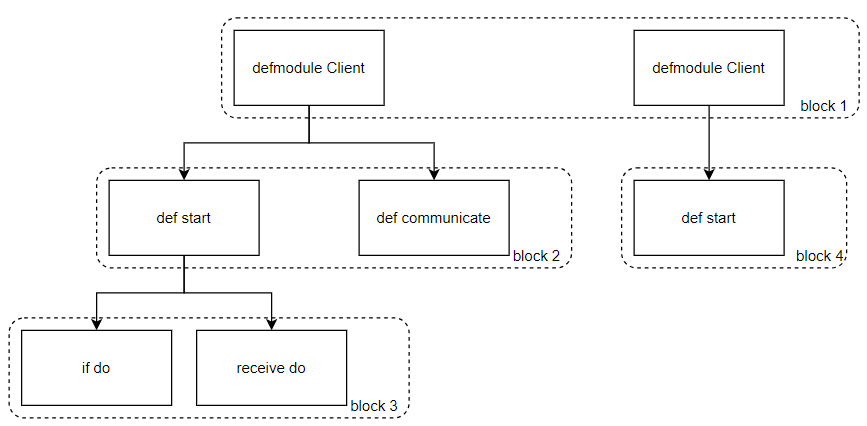
\includegraphics[width=0.8\textwidth]{images/sym_Table.png}
    \caption{An example symbol table scope hierarchy.}
    \label{fig:scope_hierarchy}
\end{figure}
\\ \\
\subsubsection{Traversal, Scoping and Variable Declarations}
So far, we assumed no expressions were matched to variables. To support assignment, we are required to track the execution of a scope in more detail. Let's first re-iterate Elixir's \texttt{match} operator and describe how the model generator handles it. Every expression in Elixir returns a value. We can match the entire expression to a single identifier, or use pattern matching to have more granular control on how the expression is deconstructed. We could also form guards for more complex checks used in conditional statements (such as \texttt{if} and \texttt{receive}). Elixir is a dynamically, strongly typed language. Dynamic typing enforces restrictions on the set of Elixir expressions we support.
\\ \\
In the intermediate representation (IR), a match is represented as either a declaration or an assignment. Given a declaration, we can infer the variable type and assign this in the symbol table. Now the variable is declared, any subsequent match in the same scope level is considered an assignment.
\\ \\
If we now match on an expression that introduces a new child scope (such as a receive or if), we must explore every possible branch, determine the returning expression of the branch and use the relevant identifiers to assign the return value to the parent scope. To achieve this, the expression is traversed in using a depth-first search with a stack of lists. The stack manages the scope nesting and the lists manage the variable identifiers. Let's explore an example.
\begin{lstlisting}[language=Elixir, xleftmargin=.1\linewidth, caption={Representing variable declarations using the match operator}.]
    {player, action} = receive do
        {:move, player, direction} -> {player, "moved #{direction}"}
        {:attack, player, target} -> 
            send health, {target, -2}
            {player, "attacked #{target}"}
    end
\end{lstlisting}
In the example, we are matching with a tuple. We push $player$ and $action$ to the identifier list and then descend into the first guard (conditioned by the \texttt{:move} atom). This is a singular expression, so it must be the return value of this guard. We can peek the scope stack to access the list of variables, and iterate through them assigning the relevant values. Assuming this is a declaration, we also add the identifiers to the current scopes symbol table. We can mark direction as a $string$ as this is easily inferred, but we leave $player$ as $unknown$ until we can gather more information about the type. We now traverse the second branch. This follows the \texttt{block} construct, so we require pushing an empty list to the stack. We recursively apply this process until we reach the last expression in the block. Reaching the last expression, we can pop the stack (removing the child scope level) and then peek the stack to access the list of variables from the parent scope. We assign these using the same method, this time asserting the types align with the symbol table, or inferring more information about $unknown$ types if possible. Figure \ref{fig:scope_hierarchy2} shows the stack and lists for the second receive guard.\\ \\
\begin{figure}[h]
    \centering
    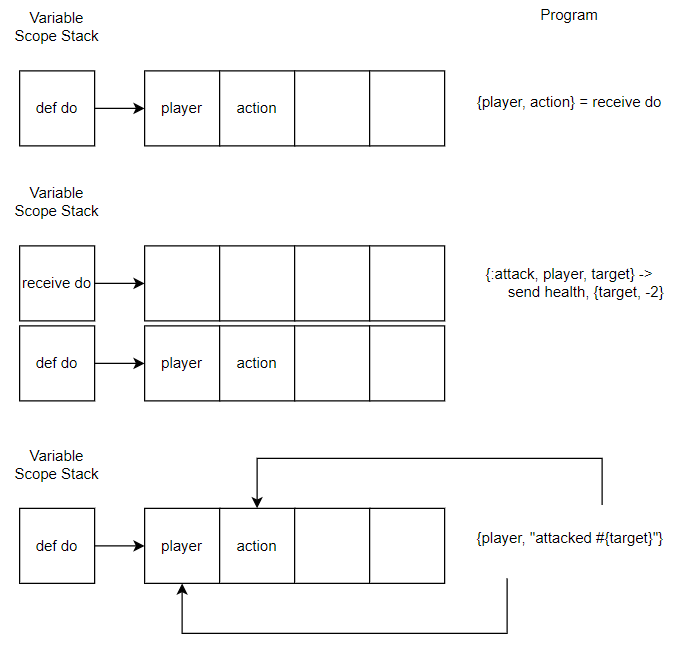
\includegraphics[width=0.7\textwidth]{images/var_stack.png}
    \caption{Example variable stack and identifier lists. The stack relates to the scope level, we push and pop as we traverse the receive guard. Only values waiting assignment are added to the identifier list.}
    \label{fig:scope_hierarchy2}
\end{figure}
\subsubsection{Functions, Type Specifications and Return Types}
Like the other constructs, functions introduce a new scope level. Multiple functions within a module can be used to determine the control flow for a process. Before we discuss about how the functions are represented, we must quickly discuss types again. A correct LTLixir specification should provide type information for all function arguments and the return type. These properties are used to aid the type inference. The return type also determines how we model our function. If the return type is \texttt{:ok}, the function is non-returning, and we can treat the function as a standard sequential execution (but with its own local internal representation). If a return type is provided, we use a similar technique, by recursively traversing expressions to determine all exit points of the function. 
\\ \\
Promela does not support functions. We model functions using Promela processes and rendezvous communication channels. To implement functions using our writer, we apply various techniques that mimick how Elixir functions behave. Firstly, the caller must declare a new rendezvous communication channel (using a buffer size of 0). A rendezvous channel has no buffer and hence communication over the channel is entirely synchronous. We also declare a new variable to store the return value of the function, typed using the type specification of the callee. We can now spawn a new process (a process mocking the function) and pass two imperative arguments, alongside the arguments specified in the Elixir function. We first pass the channel, which acts as both a return value and signalling method for the function termination. We also pass a process identifier. All processes are identified by this process id; by passing this to the callee, the callee can take actions as if it were communicating as the parent process. We then pass the remaining arguments as if we were making an Elixir function call. The caller will now block until the callee sends a message over the signalling channel. The callee can proceed as normal, and by using the discussed traversal techniques, all exit points will send the final expression over the signalling channel. This approach easily extends to recursion, as the callee can spawn a new instance of itself and block until a signal is received. In figure \ref{fig:function_call}, we show an example of a recursive function call.
\begin{figure}[h]
    \centering
    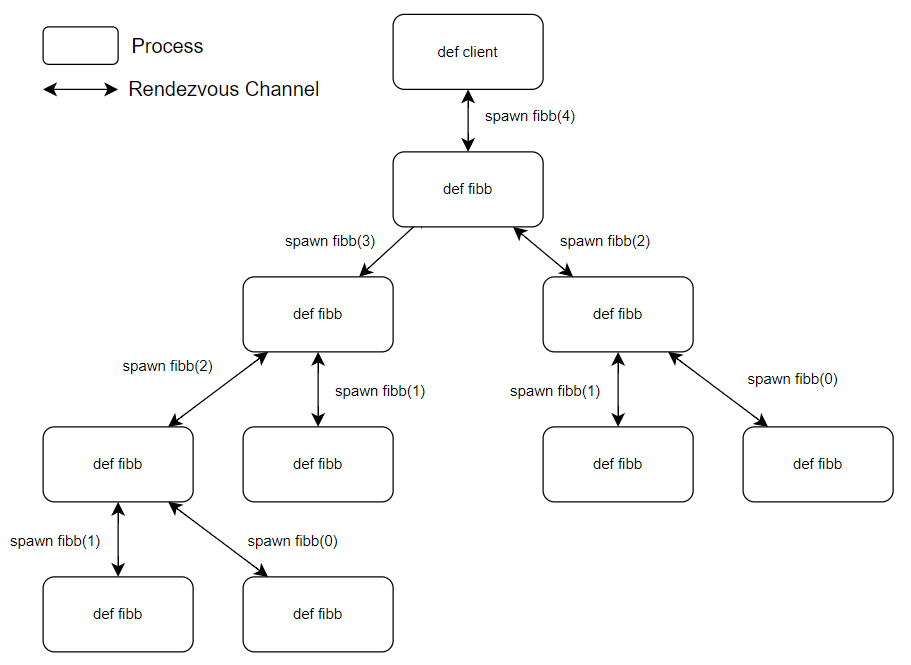
\includegraphics[width=0.8\textwidth]{images/function_call.png}
    \caption{An example of a recursive function call. In total, 9 processes are spawned to calculate the factorial of 4. Callers block until they rendezvous with callees. If we consider the call stack as a graph, it is traversed in a depth-first manner.}
    \label{fig:function_call}
\end{figure}
\subsection{Concurrent Memory Model} \label{sec:memory_model}
Now we have explored the basics of modelling Elixir programs, we extend the ideas to programs with multiple processes running concurrently. To correctly design a model of a concurrent Elixir system, there are a few core principles we must capture.
\begin{itemize}
    \item Spawning processes.
    \item Sending messages.
    \item Receiving messages.
    \item Bounding communication.
\end{itemize}
We will first explain how we model the spawning of a new process, before taking a deeper look into more complex concurrency primitives as well as a memory model to extend the existing capabilities of Promela. The Verlixir IR for spawning processes resembles the Elixir spawn very closely. We capture a function that acts as the entry to the process which we can then model as a Promela process. As with a function call, we pass a process identifier to the new child process. In this case, the process identifier is a reserved identifier that signals to the new process to take a unique process identifier assigned automatically by the system. This is an important mechanism to ensure all parents are uniquely identifiable, which is crucial for communication. This process identifier can be captured in the caller's symbol table and used to communicate with the process.
\\ \\

\subsubsection{Actors, Mailboxes and Message Passing}
Once we have another process's identifier in our symbol table, we can begin communication between processes. Elixir implements this communication using the actor model, where each running process in the system is an actor that can send messages and receive messages using a mailbox. The mailbox can be considered a first-in-first-fireable-out queue. The IR must capture this ordering, otherwise it could misrepresent the execution of an Elixir program.
\\ \\
\subsubsection{Constructing Messages}
We begin by describing the design of a message. A message is comprised of two components, the \texttt{message type} and the \texttt{message body}. In Elixir, the message type is denoted with an atom, which the IR simply treats as a distinct type within the system. When the message type is used in the context of a send or receive it is added to a global set of message types. Tracking this set globally is important to model the entirety of the system. The message body consists of multiple message arguments. At this point, the IR does not refer to the message argument by its type but purely treats it as an argument, that is expected to be passed in communication. We can store any primitive type within a message argument by inferring the type from the send or receive expression. If a type cannot be inferred in the context, we reserve a byte array to store the message argument, but to avoid this causing memory issues, we limit the size of the byte array to a small fixed size.
\\ \\
\subsubsection{Sending Message}
Now that we can construct a message, we can begin to model how messages can be sent and received. The IR keeps close to the mailbox system the actor-based implementation uses. Using the global message type set, we construct a per-process mailbox for each message type. The per-process mailboxes are constructed by passing a process identifier, as an index on the channel, where the index aligns with the process identifiers we had previously been allocating. When a process sends a message, we triage which mailbox the message should be sent to, using the message type and use the process identifier from the symbol table, to index into the correct communication channel to attach the message.
\\ \\
\begin{figure}[h]
    \centering
    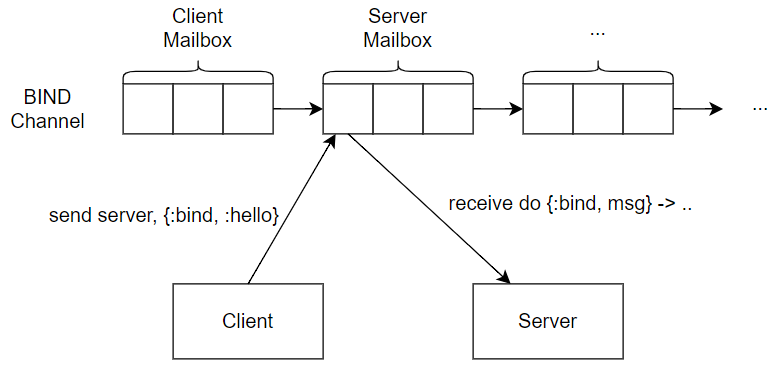
\includegraphics[width=0.8\textwidth]{images/promela_messages.png}
    \caption{An example of modelling the Elixir mailbox.}
    \label{fig:promela_mailbox}
\end{figure}
\\ \\
\subsubsection{Receiving Messages}
Receiving a message is a little more complex. We must now consider pattern matching in guard conditions. To begin pattern matching, we can again use the message type system to determine which mailbox to check. If more than just the message type is required in the pattern matching of a guard, we must pre-empt elements of the message body to determine which elements are important for pattern matching and which elements are identifiers that need assignments. In order to generate a model for the guards, we introduce a blocking statement consisting of multiple conditions. When one of the conditions is satisfied (i.e. a message has been pattern-matched) we stop blocking, execute the block relevant for the matched guard and then break out of the control structure. \\ \\
Before we can execute the block, we must assign all the remaining identifiers from the receive guard, to the relevant values in the received message body. To do this, we first introduce a new dummy variable which is assigned the value of the entire message body. We can then access the dummy variable to assign the remaining identifiers from the guard. During the assignment, we have no indication of the type of the identifier. Hence, we can temporarily assign a message argument to the identifier, and extract the correct attribute from the message argument when we have more information about the type.
\\ \\
Unlike Elixir actors, Verlixir bounds multiple communication primitives. This is to ensure state explosion in the model checker is less likely to occur. As mentioned, we are strict in the bounding of byte arrays that can be passed as message arguments. We also only supply a small number of mailboxes per message type, furthermore, we bound the number of messages that can buffer in a per-process mailbox.
\subsubsection{Dynamic Memory Allocation}
Although not a direct fallout of the Elixir concurrency prinicples, Promela does not support dynamic memory allocation such as memory allocations or memory de-allocations. This lack of support has lead to design choices in the generation of Elixir lists that if mishandled could lead to a mis-representation of Elixir concurrency in the target specification language. Immutability is a core feature of the Elixir runtime, hence the Elixir list operations introduce behaviours that must be carefully handled. For example, the \texttt{++} operator can be used to append or prepend elements to a list. If this is used to prepend, the operation is constant time, however the IR will represent this (as well as most list operations) as an operation in linear time. Let's explore the memory model to understand why. 
\\ \\
The IR introduces two structures to handle all list operations across the system. These structures are stored in the global scope context. The reason for this comes from Promela limitations. Promela supports statically sized arrays. These arrays cannot be passed to other processes. Hence, an array's lifetime is limited to its scope. To get around this limitation, the two structures we introduce are called \texttt{memory} and \texttt{linked\_list}.
\\ \\
First we describe the design of \texttt{linked\_list}. It is in fact not a traditional linked list, but it behaves similar as we can perform many operations on this structure that we could not perform on a statically size array. For example, we support prepending and appending in order to dynamically resize the list. In actuality, none of these operations resize the list. A list has an upper bound in it's size, which is statically set for all model generation. Let's name this limit L.
\begin{lstlisting}[language=C, xleftmargin=.1\linewidth, caption={The structure of a list}.]
typedef linked_list {
    node vals[L];
}
\end{lstlisting}
For example for a limit, $10$, means the maximum number of elements that can be appended to the list is 10. The list starts as empty and is handled by the \texttt{node} nested structure.
\begin{lstlisting}[language=C, xleftmargin=.1\linewidth, caption={Example of a list node typed `int'.}]
typedef node {
    int val;
    bool allocated;
}
\end{lstlisting}
A \texttt{node} stores a single value in a list, as well as a flag to indicate if the value has been allocated. Now, given a sequence of nodes, the order of the nodes represents the order of the Elixir list for all $true$ allocated nodes. For example, for a list, ls, $ls[0]$ and $ls[9]$ can be contiguous list elements, if they are both allocated and there are no allocations in between.
\\ \\
Given this representation, we now see why all operations are in linear time. For example, for insertion (prepend or append), we must assign a pointer to a node and iterate through all nodes to find an unallocated node to insert into.
\\ \\
We now extend this implementation of a dynamically sized list to introduce dynamic memory. The implementation is similar to how lists are implemented. We now introduce a new field to \texttt{linked\_list} called \texttt{allocated}. This represents the allocation of a list in memory. We now similarly introduce memory.
\begin{lstlisting}[language=C, xleftmargin=.1\linewidth, caption={Memory intermediate representation. Limit of M lists.}]
typedef memory {
    linked_list lists[M];
}
\end{lstlisting}
With this structure, we introduce a single, globally defined instance of this structure named \texttt{\_\_memory}. All processes share this singular memory for their list allocations. All list operations are treated as a single, indivisible step so this does not introduce concurrent execution concerns. If an Elixir process declares a new list, the IR will represent this as a memory allocation. The model runtime will iterate through all the lists in memory, to find an unallocated list and return this as a pointer to the process. As dynamic memory allocations are not supported in Promela, this $pointer$ is generated as an \texttt{int}, which indexes into memory. 
\\ \\
Finally, with all these definitions in place we can finally support the passing of Elixir lists as function arguments. When we detect a function call, or \texttt{send} expression passing a list, we first allocate a pointer to a new location in memory. We then copy all the values from the list into the new allocation and then pass the pointer as an argument. With this mocked memory in place, we can now support Elixir lists and operations on them. We will discuss a few of these operations next.
\\ \\
\subsubsection{Iteration and Higher Order Functions}
Promela supports for loops, but for our custom dynamic memory, these do not suffice. Using a similar approach we used to append list elements, a $for$ comprehension can be represented as a linear scan through all \texttt{linked\_list} elements. We find the allocated elements and apply the comprehension body to these. We can introduce temporary dummy variables to represent Elixir's \texttt{<-} operator. If we want to match on a $for$ comprehension, we must also introduce a pointer into a second \texttt{linked\_list} which tracks new allocations into the matched block independently of the scan through an existing list. A $for$ comprehension over an Elixir range construct, \texttt{n..m}, can be represented with a for loop.
\\ \\
A map operation (such as from the \texttt{Enum} Elixir library) is represented similarly to a $for$ comprehension in the IR. Instead of inlining the body, in order to hold a more fair representation of the Elixir program, dummy anonymous processes are stored to represent higher-order functions.
\\ \\
As a closing note on memory, we describe the representation of randomness. Again, Promela does not inherently support randomness which has influenced the IR design. To represent a function such as \texttt{random} from the \texttt{Enum} library, we represent this using multiple truth conditions, which can be selected non-deterministically. One of these conditions will return an allocated list element and one will increment the current list pointer. To ensure termination, if we point to the end of the list before returning a value, we simply return the last allocated value we saw. This is not true randomness, and is not fair to all elements in the list hence random operations are strongly discouraged in LTLixir, but are theoretically supported.
\\ \\
Note that as Promela does not support functions, when we generate a model, all of these Elixir functions are in-lined into the process body. Any reference to a function $return$ is actually simply generated as an assignment.

\subsection{Supporting LTLixir} \label{sec:supporting_ltl}
In section \ref{sec:specification_language} we discussed how Elixir was extended to support inline specifications. We now describe how these are modelled in the IR and generated in Promela.
\\ \\
\subsubsection{System Entry}
The \texttt{@init} LTLixir attribute represents an entry point to the system. We represent this using a flag in the IR for each process, determining if the process should be running in the first state of the model.
\\ \\
\subsubsection{Type Specifications}
A \texttt{@spec} attribute is parsed when parsing a function definition. For each argument being parsed when creating a new function in the IR, we insert a new symbol table entry using the type provided in the type specification. The return type is a special case of this as it could be the non-returning \texttt{:ok} type. If this is received, we insert a reserved non-returning type into the symbol table, and interface with this, by supporting a \texttt{table.returning\_function $\rightarrow$ boolean()} call to determine if a function is returning. If a function is non-returning, it would be an error to attempt to look up the type of the function in any context. If a function is returning, we must ensure all expressions which are returning (i.e. last in a block) write to the rendezvous channel, as discussed in section \ref{sec:sequential_execution}.
\\ \\
\subsubsection{Concurrency Parameters}
A \texttt{@model} attribute also instruments the IR of a function. For all of the parameters in the tuple of identifiers, we mark these before continuing with storing the remainder of the function. When a declaration of one of these identifers is found in an expression, we avoid the usual handling of this and instead assign a dummy value \texttt{\_\_PARAM} to the identifer. This dummy value is used by the model generator to create multiple configurations of a single model, which will be discussed more in section \ref{sec:simulation_verification}.
\\ \\
\subsubsection{Linear Temporal Time Formulae}
The final attribute is \texttt{@ltl}. When an LTL formula is parsed, we create a set of all identifers (or predicates) present in the formula. We first instrument the function body by marking all these identifers as LTL identifers. When we detect the declaration of an LTL identifer to an expression, we extract this declaration out of the function and move it to the global context. Internally, we now consider this a system property as opposed to a property of a single process. When we have extracted all LTL identifer declarations, we can handle the conditions of the LTL formula, such as the temporal properties. We construct formulae from the system properties using the same operators the user defined in the attribute. We finally mark these formulae as LTL formulae in the IR. This means the Promela model generator can create LTL properties to instrument the rest of the state-space during verification.
\\ \\
\subsubsection{Predicates}
Similarly to LTL properties, any predicates are tracked in a similar way. Any identifers that construct a predicate must be extracted to the global context and flagged as system properties. We also globally define the predicates using the system properties in order to ensure they are valid within an LTL formuae.
\\ \\
\subsubsection{Verifiable Functions}
The \texttt{defv} construct is handled as the the other function definitions are as described in section \ref{sec:sequential_execution}. Verifiable functions are still internally represented as processes, however we now also extract the pre- and post-conditions from the definition. A pre-condition instruments a function by inserting a truth condition to be evaluated before the rest of the function body. A post-condition flag is set in the functions definition in the event one is parsed. When a post-condition flag is set, we ensure to instrument all returning expressions of a function to assert the truth of the post-condition. As in the IR, functions write to a rendezvous channel instead of returning, we perform this violation check after the return point of a function. When the verifier is run on a model, every state in the state-space is exhaustively checked, hence any possible evaluation of a pre- or post-condition will be exhaustively checked in the verification process. This provides better assurance than relying on the condition checks during the Elixir runtime.

\section{Simulation and Verification} \label{sec:simulation_verification}
We have now explored the intermediate representation constructed by Verlixir, alongside some implementation details specific to using Promela as a target language. This section will describe the remainder of the Verlixir design, which touches on simulation, verification, generating multiple models and using Spin as a target model checker. The default execution of the Verlixir executable, will produce a single Promela model for a given input LTLixir specification. For Verlixir to produce outputs, it should be executed with a flag to set the mode: $\{-s, -v, -p\}$ for simulation, verification or parameter exploration. The flags determine how the Spin model checker is run.
\\ \\
If $-s$ is passed, Spin is run in simulation mode. If $-v$ is passed, Verlixir will first determine the existence of LTL properties within the model. For each LTL property, we run an instance of Spin specifying the LTL property we want to evaluate. We do this using Spin's $-search$ parameter, which will generate and run the verifier from the model. In the event we do not detect an LTL property, we use $-search$ to check for the existence of deadlocks or non-progress cycles (livelocks). If $-p$ is passed, multiple models are generated instead of one, and all of these are checked as if $-v$ was passed for each.
\subsection{Simulation}
Simulation mode will use the Spin scheduler to execute a single execution through the generated state-space. A simulation can timeout in the case of a deadlock. If a timeout is produced, we inform the user of the timeout but do not provide further information as that is left for verification mode. Elixir calls to the \texttt{IO} library can be re-produced in simulation mode as we display them to the user if they are executed. These are not as proficient as using \texttt{IO} in the Elixir runtime. Simulation mode can be more beneficial than examining the output of running an Elixir program. The scheduler takes enabled transitions based on the current state, whereas, the Elixir scheduler, runs in real-time, resulting in a process interleaving never being observed.
\subsection{Verification}
Verification mode will run the Spin verifier. If an error is detected, the output is captured by the Verlixir error profiler, which triages the issue to generate relevant outputs for the user to digest. For example, if a non-acceptance cycle is produced by Spin, Verlixir captures this and reports to the user that either an LTL property was violated (liveness property) or the system is potentially livelocked. Verlixir will report the entire trace that lead to this cycle, showing which process was responsible for a transition between states as well as reading from the Elixir module the line of Elixir code that lead to that transition. 
\\ \\
\subsubsection{Reporting Violations}
The mapping between Elixir expressions and how they are modelled is not a one-to-one mapping of line-numbers. Instead a single Elixir expression can result in multiple Promela expressions and multiple states in the state-space Spin traverses. Still, all the relevant Elixir expressions are captured and reported in the trace produced. For this error, Verlixir will also report the cycle that lead to non-terminating processes. It will report where the cycle begins, then give a trace of executed Elixir lines and which function executed them. The error profiler also captures and reports the processes which have terminated, or a blocking expression (such as a receive with no accepting guards). For a given model $M$, the profiler can determine the following truth conditions for the specification $\phi$. If the specification holds for an initial state, $S_i$, we have $(M, S_i) \models \phi$. If the specification holds for all initial states, the specification is valid: $M \models \phi$. The error profiler may report a violation, in which case for a violating specifiation $\phi _v$ we have $(M, S_i) \models \phi _v$. For example, deadlocks, non-accept cycles, out-of-memory, assertion violations are possible violating specifications all represented by $\phi _v \in \{\phi _{dl}, \phi _{cycle}, \phi _{memory}, \phi _{assert}\}$. In the event that $M \models \phi _{memory}$, we could re-run the verification process using directives to reduce memory usage. If this is required, Spin will no longer perform an exhaustive search. If the specification is true under these conditions, we can only say the model partially models the specification, $(M, S_i) \models \phi _p$. A non-exhaustive search should only be applied as a last resort, if it is infeasible to perform verification by reducing the system complexity and can be performed using the $-r$ flag. 
\\ \\
\subsubsection{Fairness}
Similarly, in the event $M \models \phi _{cycle}$, it may be useful to introduce weak fairness to the system. Weak fairness can be applied by passing the $-f$ flag when in verification mode. Other flavours of fairness should be introduced using LTL formulas. If the weak fairness flag is active, scheduling decisions will consider how process-level non-determinism is resolved. For example, if a non-progress cycle is detected by a single process infinitely executing, even when there are other active processes that are not being scheduled, by re-running the verifier with weak fairness applied, infinitely enabled transitions will eventually be scheduled to be taken. This may instead report a new error, consisting of a fair non-progress cycle, or even avoid the non-progress cycle entirely.  
\subsection{Parameterization}
The Verlixir IR passes all detected parameters to the Verlixir model runner. The model runner is responsible for generating multiple models depending on the number of parameters provided, $N$ and the range of search values, $M$, which can be parsed as a command line argument using $-p\text{ }M$. The model runner generates a total of $M^N$ Promela models. All of these models are ran in $-search$ mode and violations are reported. Verlixir reports an acceptance score, $\alpha$, determining how many of the models were accepted by the verifier: $\alpha \coloneq 1 - \frac{|V|}{M^N}$, where $V$ are violating models. After outputting $\alpha$, we note all the elements of $V$ so the user can generate a trace for the violation using verification mode.

\section{Modelling Paxos}
We will now demonstrate the model generation process for a larger example, the basic Paxos algorithm. A thorough explanation of the problem will be discussed in section \ref{sec:Paxos}. For now, we will just concern ourselves with the syntax of the Elixir program and how it is parsed and translated into Promela.
\\ \\
The entire program is large, so we will just look at a single Elixir $defmodule$. In particular, we will look at the $learner$ module. When the system is distributed, the $learner$ could be an Elixir node, or an Elixir process. For our model, it does not matter. We will now take a look at the Elixir implementation of one of the functions of the learner, $wait\_learned$, focusing primarily on the syntactic elements.
\\ \\
\begin{lstlisting}[language=Elixir, xleftmargin=.05\linewidth, caption={A function from the $learner$ module}.,label = lst:learner]
@spec wait_learned(list(), integer(), integer()) :: :ok
@ltl """
[]((p->!<>q) && (q->!<>p))
<>(r)
[](s)
"""
def wait_learned(acceptors, p_n, learned_n) do
    predicate p, final_value == 31
    predicate q, final_value == 42
    predicate r, final_value != 0
    predicate s, final_value == 0 || final_value == 31 || final_value == 42

    if p_n == learned_n do
        for acceptor <- acceptors do
            send acceptor, {:terminate}
        end
    else
        receive do
            {:learned, final_value} ->
            IO.puts("Learned final_value:")
            IO.puts(final_value)
        end
        wait_learned(acceptors, p_n, learned_n + 1)
    end
end
\end{lstlisting}
Listing \ref{lst:learner} shows an Elixir function, $wait\_learned$. The function specifies some LTL properties, using the multi-line LTL syntax. The LTL properties rely on the predicates defined in the function body. The function also receives some arguments. In the body, we see conditional branch, where one branch involves a $for$ comprehension, through a list performing some message sending. The other branch receives a value. At the end of the $else$ condition, we recurse. Let's now break down the Promela model.
\\ \\
\begin{lstlisting}[language=Promela, xleftmargin=.1\linewidth, caption={Promela function definition}., label=lst:func_def]
#define p ((final_value == 31))
#define q ((final_value == 42))
#define r ((final_value != 0))
#define s ((((final_value == 0) || (final_value == 31)) || (final_value == 42)))

proctype wait_learned (int acceptors;int p_n;int learned_n;chan ret;int __pid;int __ret_f) {
    chan ret1 = [1] of { int }; 
    atomic{
        if
        :: __pid == - 1 -> __pid = _pid;
        :: else -> skip;
        fi;
    }
\end{lstlisting}
Listing \ref{lst:func_def} shows the first translation result of Promela from the Elixir function. Firstly, we see the predicates are pulled from the body and placed into the global context.
\\ \\
The function is translated to a process type, named $wait\_learned$. The process receives the same arguments as the Elixir function, using the type specification to type the arguments. Additionally, we receive some meta-arguments $\_\_pid$ and $\_\_ret\_f$. The first line of the function body creates a channel, named $ret1$. Channels of this nature will be used in function calls.
\\ \\
Finally, we see an $atomic$ block, which performs a check on the received $\_\_pid$. If the process id passed is $-1$, we assign a new process id from the process scheduler. Otherwise, we continue to act as the caller, by retaining the passed process id.
Next, we look at the first branch of the Elixir $if$ statement. In particular, we will look at the $for$ comprehension.
\begin{lstlisting}[language=Promela, xleftmargin=.1\linewidth, caption={Promela if statement and for comprehension}., label=lst:for]
if
:: (p_n == learned_n) -> 
    atomic {
        __list_ptr_old = __list_ptr;
        __list_ptr = 0;
        __list_ptr_new = 0;
        do
        :: __list_ptr >= LIST_LIMIT || __list_ptr_new >= LIST_LIMIT -> 
            __list_ptr = __list_ptr_old;
            break;
        :: else -> 
            if
            :: LIST_ALLOCATED(acceptors,__list_ptr) -> 
                int acceptor;
                acceptor = LIST_VAL(acceptors,__list_ptr);
                atomic {
                    MessageList msg_0;
                    __TERMINATE!!acceptor,TERMINATE,msg_0; 
                }
                ;
                __list_ptr_new++;
                __list_ptr++;
            :: else -> __list_ptr++;
            fi
        od
    }
\end{lstlisting}
Listing \ref{lst:for} shows the translation for the $if$ statement. Each condition in the $if$ is determined with a (::) operator. In this listing, we just have the first condition, the $else$ will be seen in a later listing. 
\\ \\
Next, we have the translation of the for comprehension. This is wrapped in an atomic block, as it relies on accessing shared memory. It looks daunting, but all that is taking place is a linear scan through the list. We check each element, determine if it has been assigned and if it has, then the comprehension body (line 14 through 19) is executed with the list element.
\\ \\
In this case, the comprehension body is a $send$. To send, we pack the message elements into structure, and then send this data to the channel matching our $terminate$ atom, and the mailbox matching $acceptor$.
\\ \\
Now let's look at the $else$ condition.
\begin{lstlisting}[language=Promela, xleftmargin=.1\linewidth, caption={Promela receive and recursion}., label={lst:else}]
:: else -> 
    MessageList rec_v_5;
    do
    :: __LEARNED??eval(__pid),LEARNED,rec_v_5 -> 
        final_value = rec_v_5.m1.data2;
        printf("Learned final_value:\n");
        printf("final_value\n");
        break;
    od;
    int __temp_cp_arr_2;
    __copy_memory_to_next(__temp_cp_arr_2,acceptors);
    int __ret_placeholder_1;
    run wait_learned(acceptors,p_n,learned_n + 1,ret1,__pid,1);
    ret1?__ret_placeholder_1;
fi;
\end{lstlisting}
Listing \ref{lst:else} shows the translation of the $else$ condition. Again, this is guarded by a (::) operator. We do two things here: first we receive a message and then we recurse.
\\ \\
The receive only has one guard. We translate this guard by reading from the $learned$ channel, looking into our own mailbox (marked by $\_\_pid$). The data we read from the channel is read into $rec\_v\_5$, which we unpack into the relevant variables.
\\ \\
Secondly, we make a recursive function call. As one of the arguments passed is a list, we must ensure we pass the list by value. To do this, we get a new pointer from memory, and copy the values from our local list into the new memory location.
\\ \\
We next create a value to store the returned value from the recursive call. Actually, in this case the function's type definition marked the function as `non-returning'. We recursively call the function by spawning a new instance of the process type. We pass the parameters, as well as the relevant meta-arguments. In this case, the meta-arguments are:
\begin{itemize}
    \item The channel to send the return value to, $ret1$. This was defined at the beginning of the function body.
    \item We pass our own process id, so the spawned function can continue to take actions on our behalf.
    \item We pass $1$. $1$ marks a non-returning function.
\end{itemize}
We then wait to read on $ret1$ to rendezvous with the callee.
\\ \\
Let's finally look at the remaining translated code.
\begin{lstlisting}[language=Promela, xleftmargin=.1\linewidth, caption={Translation of LTL properties}., label={lst:final}]
    atomic  {
        if
        :: __ret_f -> ret!0;
        :: else -> skip;
        fi;
    }
}


ltl ltl_1 { []((p -> ! <> q) && (q -> ! <> p)) };
ltl ltl_2 { <> (r) };
ltl ltl_3 { [](s) };
\end{lstlisting}
Listing \ref{lst:final} shows the remainder of the translated code. To end the function, we have a final $atomic$ block. Within this block, we check the value of the passed $\_\_ret\_f$ value. If this is $1$, the function is non-returning. To handle the resolution of the call stack, we propagate a ghost $0$ through the return channels. If it was a returning function, the return would already have been handled, and hence we can $skip$.
\\ \\
Finally, after the function and back in the global context, we define our LTL properties. We split the multi-line property into multiple properties so they can be checked in parallel. They rely on the predicates defined, which were defined in the global context as they are properties of the system, not a single process.
\\ \\
\section{Summary}
This chapter has discussed some core design concepts behind LTLixir and Verlixir. We first looked at a high-level overview of where the tools fit into a wider toolchain and gave a basic introduction to their architecture. We saw how Elixir was extended using metaprogramming to support inline specifications. We then introduced the core techniques essential to constructing an intermediate representation of an LTLixir specification as well as how Promela can be used as a target modelling language for Elixir systems. Finally, we looked at how Verlixir interacts with the model checker Spin to simulate and verify programs while capturing traces of Elixir programs. We will now evaluate the effectiveness of this tooling.

\chapter{Evaluation}
In this chapter, we aim to evaluate the expressiveness of Veriflixir's design. First, we perform a quantitive analysis of modeling classical distributed algorithms such as basic paxos in section \ref{sec:paxos} and the alternating-bit protocol in section \ref{sec:ab}. Section \ref{sec:vs} will delve into a comparison against current state-of-the art model checking techniques for modern day programming languages. Finally, we will explore the performance of Veriflixir in a growing sytem in section \ref{sec:perf}.
\section{Analysing Distributed Systems}
Verifying the correctness of real-world distributed systems is a major motivation for this project. Critical real-time systems (such as in air-traffic control or healthcare  \cite{airlines,healthcare}) should not fail and should rely on rigerous verification techniques to guarantee production code is correct.  
\subsection{Basic Paxos} \label{sec:paxos}
Paxos is an example of a distributed algorithm \cite{paxos_simple}. It is a consensus algorithm, where many processes are tasked to agree on a value. Processes may propose what this value should be, but only one value should be agreed upon. The safety requirements for consensus are:
\begin{itemize}
    \item Only a value that has been proposed may be chosen.
    \item Only a single value is chosen.
    \item A process never learns that a value has been chosen unless it actually has.
\end{itemize}
The system's liveness requirement is that a proposed value is eventually chosen and if a value if chosen then a process can learn the chosen value.
\subsubsection{Informal Specification}
There are many flavors to the paxos algorithm. We will informally present a basic, one-shot paxos. 
\subsubsection{Comparison with 'Model Checking Paxos in Spin' Paper}
\subsection{Alternating-bit Protocol} \label{sec:ab}
\subsubsection{Informal Specification}
\subsubsection{Experimental Analysis}
\section{Veriflixir vs } \label{sec:vs}
\section{Performance} \label{sec:perf}
\chapter{Conclusion}
In this paper, we aimed to provide modelling and verification techniques for message-passing systems. To evaluate these techniques, we targetted Elixir, the actor-based, concurrent programming language. As part of our research, we introduced Verlixir, a verification-aware language for message-passing systems.
\\ \\
This project aimed to achieve some key objectives required for specifying and implementing distributed algorithms in a `correct' manner. The specification language supported by Verlixir, alongside Verlixir's operational modes, moves towards achieving these objectives.
\\ \\
Verlixir provides a simulator capable of simulating large-scale distributed systems. These systems can be implemented in a modern programming language, and simulated in a controlled environment. This allows developers to prototype complex systems and observe their behaviour before deploying them in a production environment. Because Verlixir directly integrates with Elixir, the system can be easily transferred from simulation to production.
\\ \\
We also have empowered developers to verify the behaviour of systems, ensuring formal safety and liveness properties are adhered to. These properties can be specified alongside the implementation of the system, and verified without the need for a separate model. Counterexamples are produced in an Elixir-friendly format, allowing developer to debug the system and understand why a property was violated; particularly focusing on the message-passing interleaving that caused the violation.
\\ \\
To extend confidence, Verlixir supports modelling systems across different configurations. This ensures systems behave consistently across different environments. This is particularly useful for distributed systems that are subject to network partitions, or systems that are required to scale up or down.
\section{Future Work}
Throughout the course of research, we have identified several areas for future work. We have indicated some of these areas previously, but we will discuss them in more detail here. An obvious extension would involve supporting a larger Elixir feature set, but we will go into depth on more unique extensions.
\\ \\
A large inspiration for this project was the verification-aware language, Dafny. The Dafny language sets out to achieve similar claims to Verlixir, but takes a different approach. Dafny fundamentally relies on theorem proving for verification, whereas Verlixir uses model checking. In particular, Dafny transpiles to Boogie, a verification-aware intermediate language. Boogie currently then uses Z3 for theorem proving. Theorem proving provides formal proofs of correctness, which give stronger claims than the pre- and post-condition checks we assert in model checking. We believe an ideal solution to verify message-passing systems could involve a combination of both theorem proving and model checking. We could extend Verlixir to support theorem proving within Elixir processes, and then continue to use model checking for verifying inter-process communication. This would provide a stronger guarantee of correctness for the system as a whole.
\\ \\
We explored the differences between Verlixir and other verification-aware languages. A key insight we drew from this is the lack of capability for injecting faults into models. Many distributed algorithms have been designed with an approach such that given there are no more than $n$ faults, the system will still follow the specification. In order to truly scrutinise these algorithms, we need the capability to inject faults into the system. A simple extension to Verlixir could involve injecting random terminating faults into processes, and then observing the system's fault tolerance under these conditions.
\\ \\
A second insight gathered from comparing tools is the lack of support for verifying computation tree logic (CTL) in modern programming languages. CTL is a temporal logic that allows us to reason about paths in a system. A simple example of where CTL could be useful is in verifying the Paxos algorithm. To ensure fairness between all proposers, we could specify and verify a CTL property that states: there exists a path where each proposal is accepted. We believe that extending Verlixir to support CTL would provide a more comprehensive verification framework for message-passing systems.
\section{Ethical Considerations}
Throughout the report we make reference to critical distributed-systems used in the contexts of air traffic control and healthcare. While the tools and research discussed are designed to improve the reliability of these systems, relying on them in isolation is not sufficient. Testing distributed systems is hard, and it is important that rigorous testing is performed by multiple parties using multiple techniques. That said, we believe Verlixir provides an advancement in the verification of distributed systems.
\section{Final Remarks}
The goal for this project was to design a tool that could verify real-world distributed algorithms which are used in research and industry. Throughout researching Verlixir, many notional examples were used to demonstrate the capabilities of the tool. Through the evaluation, we have shown these capabilities extend to real, well-known algorithms such as Paxos and Raft. In achieving this, we believe Verlixir has the potential to be a valuable tool for verifying distributed systems.
\\ \\
Historically, model checking has required hand-translation of code into a model. Verlixir lowers the barrier to entry for verifying systems. If a programmer can write their implementation using the provided LTLixir set, the system verification comes for free. We believe moving towards a world where verification-aware languages become the standard, will greatly improve the reliability of code. Instead of programmers thinking about how to implement a system, they can focus on what the system should do. A shift in mindset away from implementation specifics, towards reasoning about the safety and liveness of a system means that we can describe our systems in a more holistic way.
\\ \\
With the recent rise in artificially intelligent copilots \cite{attention_is, copilot_asset,safety_ai}, the future of programming could move towards a more declarative style. We programmers, could simply be burdened to write the system specification, in terms of safety and liveness, and a large-language model could generate the implementation.
% \chapter{Project Plan}
This chapter will discuss what needs to be done for the project to be successful, the paths that can be taken, areas that can be explored as an extension and fall-back positions in the limit of time.
\par
\section{The Artifact}
The key aim of the project is to produce a code artifact that can verify the correctness of Elixir programs. "Verify" is being used as an umbrella term for three potential components of the artifact. In no particular order:
\begin{itemize}
    \item Determining if a program is deadlock-free.
    \item Allowing users to write specifications about functions that are inline and verifiable.
    \item Verifying liveness properties. 
\end{itemize}
It would be difficult/infeasible to design a tool that can do all three from scratch and similarly, I have yet to find a tool that can do all three. Hence, my current path forward is to use a combination of existing tools where necessary to achieve these verification feats. The most appropriate tools I have identified for each case respectively are the SPIN model-checker, the Boogie IVL for theorem-proving and the TLC model-checker.
\par
Given these three tools, the plan would be to develop a command-line tool, that takes an Elixir project as an input, parses the Elixir code, and extracts the underlying model from the project to create an internal representation that can be used to generate models in the three target output grammers.
\par
The main difficulty of this project will lie in the design of Elixir. Elixir focuses on the concurrent execution of programs, using the actor model for communication between sequential processes executing in parallel. None of the target output tools have support for message passing and Boogie does not support concurrency. That means the main challenge of the project will be designing a framework for modelling programming languages that use message-passing as a first-class solution to communication. If the framework is well designed, this may not be limited to Elixir, the intermediate representation could be a target grammar that any message-passing oriented language can be translated into (such as Rust). However, for the scope of this project, modelling Elixir will be sufficient.
\par
Once a model has been extracted from an Elixir program, the next step will be code generation for the relevant tools, which can then be ran to determine the correctness of the program.
\section{Timeline and Milestones}
This section is a brief overview of what needs to happen and what has already began.
\subsubsection{Manual Translation (started)}
The first step involved understanding what an Elixir program looks like in the target representations. I spent time taking some basic Elixir programs and translating them into Promela (the specification language used by SPIN) to gather an understanding of how they can begin to be translated. I modelled four programs, an entirely sequentially executed program, a program that introduces a deadlock, a program that introduces a livelock and a program based on a deadlocking dining philosophers algorithm. While doing this, I made notes of how various components can be modelled in Promela as well as what is difficult to model. A brief summary of some findings:
\begin{itemize}
    \item In the basic deadlock model, a deadlock was detected.
    \item In the dining philosophers model (a more complex example of an Elixir program) a deadlock was detected.
    \item In the basic livelock model, the model-checker ran forever and did not detect the livelock. In theory, Promela should be detecting livelocks so more investigation needs to be done into how models need to be bound to allow for the successful detection.
    \item The key primitives unique to the actor model were able to be modelled with fair success in Promela.
\end{itemize}
As well as translating Elixir programs to Promela models, I spent some important time translating quoted expressions (equivalent to ASTs) to models, as Elixir provides the functionality to easily access them.
\subsubsection{Parsing (started)}
Parsing Elixir programs so they can be stored in an intermediate representation is important. Because of the access to quoted expressions, there is no need to parse Elixir grammar directly, instead parsing quoted expressions is easier. They are guaranteed to be well-formed, and when parsed you are left with an AST by nature. Work has begun here using a parser combinator library (pest) in Rust. The Elixir developers do not provide exhaustive documentation of the grammar of quoted expressions, so instead they have to be derived from examples and trial-and-error.
\subsubsection{Model Extraction (started)}
The main challenge of the project is model extraction. It introduces many questions that need answering:
\begin{itemize}
    \item What does a sequential execution of statements look like?
    \item How can functions be represented to be modelled in specifications that don't support functions (Promela)?
    \item How can Elixir recursion be modelled in specifications that don't support recursion (Promela)?
    \item How can concurrency processes be modelled as a sequential process (Boogie)?
    \item ho
    w can message-passing be modelled, in particular when specifications don't support shared memory?
\end{itemize}
Unfortunately, the list goes on the more you look into the Elixir language. A starting point will be modelling sequential programs.
\subsubsection{Promela code-gen (begin in term 2)}
The first model checker I aim to target is Promela. Although it doesn't natively support function calls or definitions it does support concurrency, therefore I deem it an easier milestone to reach. Once code-gen for Promela is implemented, it should be possible to begin proving Elixir programs are deadlock-free, which is a massive step towards being a verification-aware language.
\subsubsection{Extending Elixir with Metaprogramming (begin in term 3)}
It will be difficult within the scope of the project to allow any Elixir program without modification to be verified. Using metaprogramming, steps can be taken to introduce an Elixir library that allows developers to write code that is easier to verify. For example, developers can introduce bounds to mailboxes and recursive calls that make model extracting a lot more direct. Anything unbounded won't be verifiable, so I want to put the burden on the developer writing specifications instead of the artifact to approximate bounds.
\par
Metaprogramming can also be used to introduce pre- and post-conditions to Elixir to extend the support for verification.
\subsubsection{Boogie code-gen (term 3 / future work)}
After extending the Elixir language to allow the introduction of pre- and post-conditions, code-gen for Boogie programs can take place that allows stronger verification support for Elixir. I deem this an important part of the project but it depends on a lot of prior work being finished, so it's hard to determine if it fits on the timeline.
\subsubsection{Liveness (future work)}
It is unlikely that liveness will be implemented as part of the verification toolkit unless it is discovered one of the existing downstream tools supports it. I believe code-gen for a new tool will be required (such as TLA+) to achieve this, which is likely to be infeasible in the scope of the project, but on my radar.
% \chapter{Evaluation}
In this chapter, we aim to evaluate the expressiveness of Veriflixir's design. First, we perform a quantitive analysis of modeling classical distributed algorithms such as basic paxos in section \ref{sec:paxos} and the alternating-bit protocol in section \ref{sec:ab}. Section \ref{sec:vs} will delve into a comparison against current state-of-the art model checking techniques for modern day programming languages. Finally, we will explore the performance of Veriflixir in a growing sytem in section \ref{sec:perf}.
\section{Analysing Distributed Systems}
Verifying the correctness of real-world distributed systems is a major motivation for this project. Critical real-time systems (such as in air-traffic control or healthcare  \cite{airlines,healthcare}) should not fail and should rely on rigerous verification techniques to guarantee production code is correct.  
\subsection{Basic Paxos} \label{sec:paxos}
Paxos is an example of a distributed algorithm \cite{paxos_simple}. It is a consensus algorithm, where many processes are tasked to agree on a value. Processes may propose what this value should be, but only one value should be agreed upon. The safety requirements for consensus are:
\begin{itemize}
    \item Only a value that has been proposed may be chosen.
    \item Only a single value is chosen.
    \item A process never learns that a value has been chosen unless it actually has.
\end{itemize}
The system's liveness requirement is that a proposed value is eventually chosen and if a value if chosen then a process can learn the chosen value.
\subsubsection{Informal Specification}
There are many flavors to the paxos algorithm. We will informally present a basic, one-shot paxos. 
\subsubsection{Comparison with 'Model Checking Paxos in Spin' Paper}
\subsection{Alternating-bit Protocol} \label{sec:ab}
\subsubsection{Informal Specification}
\subsubsection{Experimental Analysis}
\section{Veriflixir vs } \label{sec:vs}
\section{Performance} \label{sec:perf}
\begin{thebibliography}{9}
\bibitem{csp}
Communicating Sequential Processes
Available from: \url{http://www.usingcsp.com/cspbook.pdf}.
\bibitem{pat}
Process Analysis Toolkit (PAT) 3.5 User Manual
Available from: \url{https://pat.comp.nus.edu.sg/wp-source/resources/OnlineHelp/pdf/Help.pdf}.
\bibitem{blast}
The software model checker BLAST
Available from: \url{https://www.sosy-lab.org/research/pub/2007-STTT.The_Software_Model_Checker_BLAST.pdf}.
\bibitem{prism}
PRISM Model Checker
Available from: \url{https://www.prismmodelchecker.org/}.
\bibitem{tla}
Lamport L. The temporal logic of actions. ACM Transactions on Programming Languages and Systems (TOPLAS). 1994 May 1;16(3):872-923.
Available from: \url{https://lamport.azurewebsites.net/pubs/lamport-actions.pdf}.
\bibitem{tlaplus}
Lamport L. Specifying concurrent systems with TLA+. Calculational System Design. 1999 Apr 23:183-247.Available from: \url{https://lamport.azurewebsites.net/tla/xmxx01-06-27.pdf}.
\bibitem{tlc}
Yu Y, Manolios P, Lamport L. Model checking TLA+ specifications. InAdvanced Research Working Conference on Correct Hardware Design and Verification Methods 1999 Sep 27 (pp. 54-66). Berlin, Heidelberg: Springer Berlin Heidelberg.Available from: \url{https://lamport.azurewebsites.net/pubs/yuanyu-model-checking.pdf}.
\bibitem{pluscal}
Lamport L. The PlusCal algorithm language. InInternational Colloquium on Theoretical Aspects of Computing 2009 Aug 16 (pp. 36-60). Berlin, Heidelberg: Springer Berlin Heidelberg.Available from: \url{https://lamport.azurewebsites.net/pubs/pluscal.pdf}.
\bibitem{spin}
The Model Checker SPIN
Available from: \url{https://spinroot.com/spin/Doc/ieee97.pdf}.
\bibitem{go}
Build simple, secure, scalable systems with Go
Available from: \url{https://go.dev/}.
\bibitem{elixir}
Elixir is a dynamic, functional language for building scalable and maintainable applications.
Available from: \url{https://elixir-lang.org/}.
\bibitem{beam}
A brief introduction to BEAM
Available from: \url{https://www.erlang.org/blog/a-brief-beam-primer/}.
\bibitem{erlang}
Practical functional programming for a parallel world
Available from: \url{https://www.erlang.org/}.
\bibitem{phoenix}
Phoenix Peace of mind from prototype to production
Available from: \url{https://phoenixframework.org/}.
\bibitem{discord}
Discord
Available from: \url{https://discord.com/}.
\bibitem{ft}
Financial Times
Available from: \url{https://www.ft.com/}.
\bibitem{shared_memory_verification}
Mediero Iturrioz J. Verification of Concurrent Programs in Dafny.
Available from: \url{https://addi.ehu.es/bitstream/handle/10810/23803/Report.pdf?isAllowed=y&sequence=2}.
\bibitem{dafny}
The Dafny Programming and Verification Language
Available from: \url{dafny.org}
\bibitem{defmacro}
Elixir, Macros, Our First Macro
Available from: \url{https://hexdocs.pm/elixir/macros.html#our-first-macro}.
\bibitem{z3}
De Moura L, Bjørner N. Z3: An efficient SMT solver. InInternational conference on Tools and Algorithms for the Construction and Analysis of Systems 2008 Mar 29 (pp. 337-340). Berlin, Heidelberg: Springer Berlin Heidelberg.
Available from: \url{https://link.springer.com/content/pdf/10.1007/978-3-540-78800-3_24.pdf}.
\bibitem{hoare_logic}
Hoare CA. An axiomatic basis for computer programming. Communications of the ACM. 1969 Oct 1;12(10):576-80.
Available from: \url{https://dl.acm.org/doi/10.1145/363235.363259}
\bibitem{lean}
Lean and its Mathematical library
Available from: \url{https://leanprover-community.github.io/}.
\bibitem{dialyzer}
dialyzer
Available from: \url{https://www.erlang.org/doc/man/dialyzer.html}.
\bibitem{dafny_paper}
Leino KR. Dafny: An automatic program verifier for functional correctness. InInternational conference on logic for programming artificial intelligence and reasoning 2010 Apr 25 (pp. 348-370). Berlin, Heidelberg: Springer Berlin Heidelberg.
Available from: \url{https://link.springer.com/chapter/10.1007/978-3-642-17511-4_20}.
\bibitem{dafny_tutorial}
Nipkow T. Getting started with Dafny: A guide. Software Safety and Security: Tools for Analysis and Verification. 2012;33:152.
Available from: \url{https://dafny.org/dafny/OnlineTutorial/guide}.
\bibitem{boogie}
Barnett M, Chang BY, DeLine R, Jacobs B, Leino KR. Boogie: A modular reusable verifier for object-oriented programs. InFormal Methods for Components and Objects: 4th International Symposium, FMCO 2005, Amsterdam, The Netherlands, November 1-4, 2005, Revised Lectures 4 2006 (pp. 364-387). Springer Berlin Heidelberg.
Available from: \url{https://link.springer.com/chapter/10.1007/11804192_17}.
\bibitem{csp_paper}
Hoare CA. Communicating sequential processes. Englewood Cliffs: Prentice-hall; 1985 Jan.
\bibitem{distributed_algorithms_na_lynch}
Lynch NA. Distributed algorithms. Elsevier; 1996 Apr 16.
Available from: \url{https://lib.fbtuit.uz/assets/files/5.-NancyA.Lynch.DistributedAlgorithms.pdf}.
\bibitem{model_checking}
Clarke EM. Model checking. InFoundations of Software Technology and Theoretical Computer Science: 17th Conference Kharagpur, India, December 18-20, 1997 Proceedings 17 1997 (pp. 54-56). Springer Berlin Heidelberg.
\bibitem{actor}
Agha G. Actors: a model of concurrent computation in distributed systems. MIT press; 1986 Dec 17.
\bibitem{elixir_links}
Available from: \url{https://hexdocs.pm/elixir/processes.html#links}
\bibitem{art_of_multiprocessor_programming}
Herlihy, M. \& Shavit, N. (2008), The art of multiprocessor programming. , Morgan Kaufmann.
Available from: \url{https://cs.ipm.ac.ir/asoc2016/Resources/Theartofmulticore.pdf}
\bibitem{sc}
Lamport, 1979. How to make a multiprocessor computer that correctly executes multiprocess programs. IEEE transactions on computers, 100(9), pp.690-691.
\bibitem{kripke}
Kripke, S.A., 1980. Naming and necessity. Harvard University Press.
\bibitem{temporal_and_modal_logic}
Emerson, E.A., 1990. Temporal and modal logic. In Formal Models and Semantics (pp. 995-1072). Elsevier.
\bibitem{principles_of_model_checking}
Baier, C. and Katoen, J.P., 2008. Principles of model checking. MIT press.
\bibitem{modelling_and_reasoning_about_systems}
Huth, M. and Ryan, M., 2004. Logic in Computer Science: Modelling and reasoning about systems. Cambridge university press.
\bibitem{atl}
Alur, R., Henzinger, T.A. and Kupferman, O., 2002. Alternating-time temporal logic. Journal of the ACM (JACM), 49(5), pp.672-713.
\bibitem{airlines}
Smith, P.J., Spencer, A.L. and Billings, C.E., 2007. Strategies for designing distributed systems: case studies in the design of an air traffic management system. Cognition, Technology \& Work, 9, pp.39-49.
\bibitem{healthcare}
Sarkar, B.K. and Sana, S.S., 2020. A conceptual distributed framework for improved and secured healthcare system. International Journal of Healthcare Management, 13(sup1), pp.74-87.
\bibitem{paxos_simple}
Lamport, L., 2001. Paxos made simple. ACM SIGACT News (Distributed Computing Column) 32, 4 (Whole Number 121, December 2001), pp.51-58.
\bibitem{paxos_pseudocode}
Marzullo, K., Mei, A. and Meling, H., 2013. A simpler proof for paxos and fast paxos. Course notes.
\bibitem{c_to_promela}
Jiang, K., 2009. Model checking c programs by translating c to promela.
\bibitem{gomela}
Dilley, N. and Lange, J., 2020. Bounded verification of message-passing concurrency in Go using Promela and Spin. arXiv preprint arXiv:2004.01323.
\bibitem{binary_session_types}
Tabone, G. and Francalanza, A., 2022. Session Fidelity for ElixirST: A Session-Based Type System for Elixir Modules. arXiv preprint arXiv:2208.04631.
\bibitem{proper}
Hebert, F., 2019. Property-Based Testing with PropEr, Erlang, and Elixir: Find Bugs Before Your Users Do.
\bibitem{dynamo}
DeCandia, G., Hastorun, D., Jampani, M., Kakulapati, G., Lakshman, A., Pilchin, A., Sivasubramanian, S., Vosshall, P. and Vogels, W., 2007. Dynamo: Amazon's highly available key-value store. ACM SIGOPS operating systems review, 41(6), pp.205-220.
\bibitem{consistent_hash}
Karger, D., Lehman, E., Leighton, T., Panigrahy, R., Levine, M. and Lewin, D., 1997, May. Consistent hashing and random trees: Distributed caching protocols for relieving hot spots on the world wide web. In Proceedings of the twenty-ninth annual ACM symposium on Theory of computing (pp. 654-663).
\bibitem{spanner}
Corbett, J.C., Dean, J., Epstein, M., Fikes, A., Frost, C., Furman, J.J., Ghemawat, S., Gubarev, A., Heiser, C., Hochschild, P. and Hsieh, W., 2013. Spanner: Google’s globally distributed database. ACM Transactions on Computer Systems (TOCS), 31(3), pp.1-22.
\bibitem{promela}
The Concise Promela Reference.
Available from: \url{https://spinroot.com/spin/Man/Quick.html}.
\bibitem{dafny_concurrency}
Leino, K.R.M., 2018. Modeling concurrency in Dafny. In Engineering Trustworthy Software Systems: Third International School, SETSS 2017, Chongqing, China, April 17–22, 2017, Tutorial Lectures 3 (pp. 115-142). Springer International Publishing.
\bibitem{raft}
Ongaro, D. and Ousterhout, J., 2014. In search of an understandable consensus algorithm. In 2014 USENIX annual technical conference (USENIX ATC 14) (pp. 305-319).
\bibitem{jpf}
Havelund, K. and Pressburger, T., 2000. Model checking java programs using java pathfinder. International Journal on Software Tools for Technology Transfer, 2, pp.366-381.
\bibitem{basic_paxos}
Chandra, T.D., Griesemer, R. and Redstone, J., 2007, August. Paxos made live: an engineering perspective. In Proceedings of the twenty-sixth annual ACM symposium on Principles of distributed computing (pp. 398-407).
\bibitem{ab_protocol}
Schwartz, R.L. and Melliar-Smith, P.M., 1981, April. Temporal logic specification of distributed systems. In ICDCS (pp. 446-454).
\end{thebibliography}
\appendix
\chapter{First Appendix}
\section{Verlixir Example}

\begin{lstlisting}[language=Elixir, xleftmargin=.1\linewidth]
  import VaeLib

  defmodule Server do
    @vae_init true
    @ltl "(q)U([]p)"
    @spec start_server() :: :ok
    @params {:number_of_rounds}
    def start_server do
      predicate p, alive_clients == client_n * number_of_rounds
      predicate q, !p
      client_n = 1
      number_of_rounds = 2
      alive_clients = 0
      for _ <- 1..client_n do
        client = spawn(Client, :start_client, [])
        send(client, {:bind, self(), number_of_rounds})
      end
      alive_clients = if number_of_rounds > 1 do
        check_clients(client_n * number_of_rounds, alive_clients)
      else
        0
      end
    end
  
    @spec check_clients(integer(), integer()) :: integer()
    def check_clients(expected_clients, current_clients) do
      if expected_clients == current_clients do
        current_clients
      else
        receive do
          {:im_alive} -> check_clients(expected_clients, current_clients + 1)
        end
      end
    end
  end
  
  defmodule Client do
    @spec start_client() :: :ok
    def start_client do
      {server, rounds} = receive do
        {:bind, sender, round_limit} -> {sender, round_limit}
      end
      next_round(server, rounds)
    end
  
    @spec next_round(pid(), integer()) :: :ok
    defv next_round(server, rounds), pre: rounds >= 0 do
      if rounds == 0 do
        :ok
      else
        send(server, {:im_alive})
        next_round(server, rounds - 1)
      end
    end
  end
  
\end{lstlisting}

\section{Paxos}
\subsubsection{First paxos implementation with a bug}
\begin{lstlisting}[language=Elixir, xleftmargin=.1\linewidth]
import VaeLib

defmodule Acceptor do

  @spec start_acceptor() :: :ok
  def start_acceptor do
    acceptedProposal = -1
    acceptedValue = -1
    minProposal = -1
    accept_handler(acceptedProposal, acceptedValue, minProposal)
  end

  @spec accept_handler(integer(), integer(), integer()) :: :ok
  def accept_handler(acceptedProposal, acceptedValue, minProposal) do
    receive do
      {:prepare, n, proposer} ->
        if n > minProposal do
          send proposer, {:promise, acceptedProposal, acceptedValue}
          accept_handler(acceptedProposal, acceptedValue, n)
        else
          send proposer, {:promise, acceptedProposal, acceptedValue}
          accept_handler(acceptedProposal, acceptedValue, minProposal)
        end
      {:accept, n, value, proposer} ->
        if n >= minProposal do
          send proposer, {:accepted, n}
          accept_handler(n, value, n)
        else
          send proposer, {:accepted, minProposal}
          accept_handler(acceptedProposal, acceptedValue, minProposal)
        end
      {:terminate} ->
        IO.puts("Terminating acceptor")
    end
  end
end

defmodule Proposer do
  @spec start_proposer() :: :ok
  def start_proposer do
    receive do
      {:bind, acceptors, proposal_n, value, maj, learner} -> proposer_handler(acceptors, proposal_n, value, maj, learner)
    end
  end

  @spec proposer_handler(list(), integer(), integer(), integer(), integer()) :: :ok
  def proposer_handler(acceptors, proposal_n, value, maj, learner) do
    for acceptor <- acceptors do
      send acceptor, {:prepare, proposal_n, self()}
    end

    receive_prepared(proposal_n, value, maj, 0, 0)
    {prepared_n, prepared_value} = receive do
      {:majority_prepared, n, v} -> {n, v}
    end

    for acceptor <- acceptors do
      send acceptor, {:accept, prepared_n, prepared_value, self()}
    end

    accepted_n = receive_accepted(maj, prepared_n, 0, 0)

    if accepted_n != -1 do
      # Value chosen
      send learner, {:learned, prepared_value}
    else
      # Value was rejected
      send learner, {:learned, 0}
    end
  end

  @spec receive_prepared(integer(), integer(), integer(), integer(), integer()) :: :ok
  def receive_prepared(proposal_n, value, maj, highest_seen_proposal, count) do
    if count >= maj do
      send self(), {:majority_prepared, proposal_n, value}
    else
      receive do
        {:promise, acceptedProposal, acceptedValue} ->
          if acceptedValue != -1 && acceptedProposal > highest_seen_proposal do
            receive_prepared(proposal_n, acceptedValue, maj, acceptedProposal, count + 1)
          else
            receive_prepared(proposal_n, value, maj, highest_seen_proposal, count + 1)
          end
      end
    end
  end

  @spec receive_accepted(integer(), integer(), integer(), integer()) :: integer()
  def receive_accepted(maj, prepared_n, rejections, count) do
    if count >= maj do
      if rejections >= maj do  # BUG IS HERE
        -1
      else
        prepared_n
      end
    else
      receive do
        {:accepted, n} ->
          if n > prepared_n do
            receive_accepted(maj, prepared_n, rejections + 1, count + 1)
          else
            receive_accepted(maj, prepared_n, rejections, count + 1)
          end
      end
    end
  end
end

defmodule Learner do

  @spec start() :: :ok
  @vae_init true
  def start do
    n_acceptors = 3
    quorum = 2
    n_proposers = 2
    vals = [42, 31]
    acceptors = for _ <- 1..n_acceptors do
      spawn(Acceptor, :start_acceptor, [])
    end

    for i <- 1..n_proposers do
      proposer = spawn(Proposer, :start_proposer, [])
      val_i = i - 1
      val = Enum.at(vals, val_i)
      send proposer, {:bind, acceptors, i, val, quorum, self()}
    end
    wait_learned(acceptors, n_proposers, 0)
  end

  @spec wait_learned(list(), integer(), integer()) :: :ok
  @ltl """
  []((p->!<>q) && (q->!<>p))
  <>(r)
  [](s)
  """
  def wait_learned(acceptors, p_n, learned_n) do
    predicate p, final_value == 31
    predicate q, final_value == 42
    predicate r, final_value != 0
    predicate s, final_value == 0 || final_value == 31 || final_value == 42

    if p_n == learned_n do
      for acceptor <- acceptors do
        send acceptor, {:terminate}
      end
    else
      receive do
        {:learned, final_value} ->
          IO.puts("Learned final_value:")
          IO.puts(final_value)
      end
      wait_learned(acceptors, p_n, learned_n + 1)
    end
  end
end

\end{lstlisting}

\subsubsection{First paxos bug message log}
\begin{lstlisting}[xleftmargin=.01\linewidth, xrightmargin=0.01\linewidth, caption={Message passing caused by the proposer's protocol bug.}, label={lst:paxos_bug}]
    Never claim moves to line 6     [(1)]
138:    proc  7 (start_proposer:1) test_out.pml:314 Recv 7,BIND,0,0,2,0,0,0,0,0,1,0,0,0,0,0,42,0,0,0,0,0,2,0,0,0,0,0,0,0,0,0,0,0,0,0,0,0        <- queue 20 (__BIND)
154:    proc  8 (proposer_handler:1) test_out.pml:350 Send 1,PREPARE,0,0,1,0,0,0,0,0,7,0,0,0,0,0,0,0,0,0,0,0,0,0,0,0,0,0,0,0,0,0,0,0,0,0,0,0    -> queue 23 (__PREPARE)
158:    proc  8 (proposer_handler:1) test_out.pml:350 Send 3,PREPARE,0,0,1,0,0,0,0,0,7,0,0,0,0,0,0,0,0,0,0,0,0,0,0,0,0,0,0,0,0,0,0,0,0,0,0,0    -> queue 23 (__PREPARE)
162:    proc  8 (proposer_handler:1) test_out.pml:350 Send 5,PREPARE,0,0,1,0,0,0,0,0,7,0,0,0,0,0,0,0,0,0,0,0,0,0,0,0,0,0,0,0,0,0,0,0,0,0,0,0    -> queue 23 (__PREPARE)
197:    proc  6 (accept_handler:1) test_out.pml:262 Recv 5,PREPARE,0,0,1,0,0,0,0,0,7,0,0,0,0,0,0,0,0,0,0,0,0,0,0,0,0,0,0,0,0,0,0,0,0,0,0,0      <- queue 23 (__PREPARE)
203:    proc  6 (accept_handler:1) test_out.pml:272 Send 7,PROMISE,0,0,-1,0,0,0,0,0,-1,0,0,0,0,0,0,0,0,0,0,0,0,0,0,0,0,0,0,0,0,0,0,0,0,0,0,0    -> queue 26 (__PROMISE)
205:    proc  9 (receive_prepared:1) test_out.pml:425 Recv 7,PROMISE,0,0,-1,0,0,0,0,0,-1,0,0,0,0,0,0,0,0,0,0,0,0,0,0,0,0,0,0,0,0,0,0,0,0,0,0,0  <- queue 26 (__PROMISE)
219:    proc  2 (accept_handler:1) test_out.pml:262 Recv 1,PREPARE,0,0,1,0,0,0,0,0,7,0,0,0,0,0,0,0,0,0,0,0,0,0,0,0,0,0,0,0,0,0,0,0,0,0,0,0      <- queue 23 (__PREPARE)
262:    proc  4 (accept_handler:1) test_out.pml:262 Recv 3,PREPARE,0,0,1,0,0,0,0,0,7,0,0,0,0,0,0,0,0,0,0,0,0,0,0,0,0,0,0,0,0,0,0,0,0,0,0,0      <- queue 23 (__PREPARE)
278:    proc  0 (:init::1) test_out.pml:521 Send 10,BIND,0,0,3,0,0,0,0,0,2,0,0,0,0,0,31,0,0,0,0,0,2,0,0,0,0,0,0,0,0,0,0,0,0,0,0,0       -> queue 20 (__BIND)
292:    proc  4 (accept_handler:1) test_out.pml:272 Send 7,PROMISE,0,0,-1,0,0,0,0,0,-1,0,0,0,0,0,0,0,0,0,0,0,0,0,0,0,0,0,0,0,0,0,0,0,0,0,0,0    -> queue 26 (__PROMISE)
300:    proc 11 (receive_prepared:1) test_out.pml:425 Recv 7,PROMISE,0,0,-1,0,0,0,0,0,-1,0,0,0,0,0,0,0,0,0,0,0,0,0,0,0,0,0,0,0,0,0,0,0,0,0,0,0  <- queue 26 (__PROMISE)
344:    proc  2 (accept_handler:1) test_out.pml:272 Send 7,PROMISE,0,0,-1,0,0,0,0,0,-1,0,0,0,0,0,0,0,0,0,0,0,0,0,0,0,0,0,0,0,0,0,0,0,0,0,0,0    -> queue 26 (__PROMISE)
346:    proc 10 (start_proposer:1) test_out.pml:314 Recv 10,BIND,0,0,3,0,0,0,0,0,2,0,0,0,0,0,31,0,0,0,0,0,2,0,0,0,0,0,0,0,0,0,0,0,0,0,0,0       <- queue 20 (__BIND)
370:    proc 14 (receive_prepared:1) test_out.pml:421 Send 7,MAJORITY_PREPARED,0,0,1,0,0,0,0,0,42,0,0,0,0,0,0,0,0,0,0,0,0,0,0,0,0,0,0,0,0,0,0,0,0,0,0,0 -> queue 46 (__MAJORITY_PREPARED)
372:    proc  8 (proposer_handler:1) test_out.pml:363 Recv 7,MAJORITY_PREPARED,0,0,1,0,0,0,0,0,42,0,0,0,0,0,0,0,0,0,0,0,0,0,0,0,0,0,0,0,0,0,0,0,0,0,0,0 <- queue 46 (__MAJORITY_PREPARED)
382:    proc  8 (proposer_handler:1) test_out.pml:386 Send 1,ACCEPT,0,0,1,0,0,0,0,0,42,0,0,0,0,0,7,0,0,0,0,0,0,0,0,0,0,0,0,0,0,0,0,0,0,0,0,0    -> queue 47 (__ACCEPT)
386:    proc  8 (proposer_handler:1) test_out.pml:386 Send 3,ACCEPT,0,0,1,0,0,0,0,0,42,0,0,0,0,0,7,0,0,0,0,0,0,0,0,0,0,0,0,0,0,0,0,0,0,0,0,0    -> queue 47 (__ACCEPT)
390:    proc  8 (proposer_handler:1) test_out.pml:386 Send 5,ACCEPT,0,0,1,0,0,0,0,0,42,0,0,0,0,0,7,0,0,0,0,0,0,0,0,0,0,0,0,0,0,0,0,0,0,0,0,0    -> queue 47 (__ACCEPT)
421:    proc 15 (proposer_handler:1) test_out.pml:350 Send 1,PREPARE,0,0,2,0,0,0,0,0,10,0,0,0,0,0,0,0,0,0,0,0,0,0,0,0,0,0,0,0,0,0,0,0,0,0,0,0   -> queue 23 (__PREPARE)
425:    proc 15 (proposer_handler:1) test_out.pml:350 Send 3,PREPARE,0,0,2,0,0,0,0,0,10,0,0,0,0,0,0,0,0,0,0,0,0,0,0,0,0,0,0,0,0,0,0,0,0,0,0,0   -> queue 23 (__PREPARE)
429:    proc 15 (proposer_handler:1) test_out.pml:350 Send 5,PREPARE,0,0,2,0,0,0,0,0,10,0,0,0,0,0,0,0,0,0,0,0,0,0,0,0,0,0,0,0,0,0,0,0,0,0,0,0   -> queue 23 (__PREPARE)
452:    proc 16 (accept_handler:1) test_out.pml:262 Recv 1,PREPARE,0,0,2,0,0,0,0,0,10,0,0,0,0,0,0,0,0,0,0,0,0,0,0,0,0,0,0,0,0,0,0,0,0,0,0,0     <- queue 23 (__PREPARE)
458:    proc 16 (accept_handler:1) test_out.pml:272 Send 10,PROMISE,0,0,-1,0,0,0,0,0,-1,0,0,0,0,0,0,0,0,0,0,0,0,0,0,0,0,0,0,0,0,0,0,0,0,0,0,0   -> queue 26 (__PROMISE)
460:    proc 12 (accept_handler:1) test_out.pml:282 Recv 5,ACCEPT,0,0,1,0,0,0,0,0,42,0,0,0,0,0,7,0,0,0,0,0,0,0,0,0,0,0,0,0,0,0,0,0,0,0,0,0      <- queue 47 (__ACCEPT)
466:    proc 12 (accept_handler:1) test_out.pml:291 Send 7,ACCEPTED,0,0,1,0,0,0,0,0,0,0,0,0,0,0,0,0,0,0,0,0,0,0,0,0,0,0,0,0,0,0,0,0,0,0,0,0     -> queue 48 (__ACCEPTED)
474:    proc 17 (accept_handler:1) test_out.pml:282 Recv 1,ACCEPT,0,0,1,0,0,0,0,0,42,0,0,0,0,0,7,0,0,0,0,0,0,0,0,0,0,0,0,0,0,0,0,0,0,0,0,0      <- queue 47 (__ACCEPT)
492:    proc 17 (accept_handler:1) test_out.pml:296 Send 7,ACCEPTED,0,0,2,0,0,0,0,0,0,0,0,0,0,0,0,0,0,0,0,0,0,0,0,0,0,0,0,0,0,0,0,0,0,0,0,0     -> queue 48 (__ACCEPTED)
494:    proc 13 (accept_handler:1) test_out.pml:262 Recv 3,PREPARE,0,0,2,0,0,0,0,0,10,0,0,0,0,0,0,0,0,0,0,0,0,0,0,0,0,0,0,0,0,0,0,0,0,0,0,0     <- queue 23 (__PREPARE)
500:    proc 13 (accept_handler:1) test_out.pml:272 Send 10,PROMISE,0,0,-1,0,0,0,0,0,-1,0,0,0,0,0,0,0,0,0,0,0,0,0,0,0,0,0,0,0,0,0,0,0,0,0,0,0   -> queue 26 (__PROMISE)
512:    proc 18 (receive_accepted:1) test_out.pml:459 Recv 7,ACCEPTED,0,0,1,0,0,0,0,0,0,0,0,0,0,0,0,0,0,0,0,0,0,0,0,0,0,0,0,0,0,0,0,0,0,0,0,0   <- queue 48 (__ACCEPTED)
542:    proc 21 (accept_handler:1) test_out.pml:262 Recv 5,PREPARE,0,0,2,0,0,0,0,0,10,0,0,0,0,0,0,0,0,0,0,0,0,0,0,0,0,0,0,0,0,0,0,0,0,0,0,0     <- queue 23 (__PREPARE)
554:    proc 20 (receive_prepared:1) test_out.pml:425 Recv 10,PROMISE,0,0,-1,0,0,0,0,0,-1,0,0,0,0,0,0,0,0,0,0,0,0,0,0,0,0,0,0,0,0,0,0,0,0,0,0,0 <- queue 26 (__PROMISE)
560:    proc 23 (accept_handler:1) test_out.pml:282 Recv 3,ACCEPT,0,0,1,0,0,0,0,0,42,0,0,0,0,0,7,0,0,0,0,0,0,0,0,0,0,0,0,0,0,0,0,0,0,0,0,0      <- queue 47 (__ACCEPT)
578:    proc 23 (accept_handler:1) test_out.pml:296 Send 7,ACCEPTED,0,0,2,0,0,0,0,0,0,0,0,0,0,0,0,0,0,0,0,0,0,0,0,0,0,0,0,0,0,0,0,0,0,0,0,0     -> queue 48 (__ACCEPTED)
580:    proc 21 (accept_handler:1) test_out.pml:272 Send 10,PROMISE,0,0,1,0,0,0,0,0,42,0,0,0,0,0,0,0,0,0,0,0,0,0,0,0,0,0,0,0,0,0,0,0,0,0,0,0    -> queue 26 (__PROMISE)
582:    proc 24 (receive_prepared:1) test_out.pml:425 Recv 10,PROMISE,0,0,-1,0,0,0,0,0,-1,0,0,0,0,0,0,0,0,0,0,0,0,0,0,0,0,0,0,0,0,0,0,0,0,0,0,0 <- queue 26 (__PROMISE)
602:    proc 25 (receive_prepared:1) test_out.pml:421 Send 10,MAJORITY_PREPARED,0,0,2,0,0,0,0,0,31,0,0,0,0,0,0,0,0,0,0,0,0,0,0,0,0,0,0,0,0,0,0,0,0,0,0,0        -> queue 46 (__MAJORITY_PREPARED)
616:    proc 15 (proposer_handler:1) test_out.pml:363 Recv 10,MAJORITY_PREPARED,0,0,2,0,0,0,0,0,31,0,0,0,0,0,0,0,0,0,0,0,0,0,0,0,0,0,0,0,0,0,0,0,0,0,0,0        <- queue 46 (__MAJORITY_PREPARED)
626:    proc 15 (proposer_handler:1) test_out.pml:386 Send 1,ACCEPT,0,0,2,0,0,0,0,0,31,0,0,0,0,0,10,0,0,0,0,0,0,0,0,0,0,0,0,0,0,0,0,0,0,0,0,0   -> queue 47 (__ACCEPT)
630:    proc 15 (proposer_handler:1) test_out.pml:386 Send 3,ACCEPT,0,0,2,0,0,0,0,0,31,0,0,0,0,0,10,0,0,0,0,0,0,0,0,0,0,0,0,0,0,0,0,0,0,0,0,0   -> queue 47 (__ACCEPT)
634:    proc 15 (proposer_handler:1) test_out.pml:386 Send 5,ACCEPT,0,0,2,0,0,0,0,0,31,0,0,0,0,0,10,0,0,0,0,0,0,0,0,0,0,0,0,0,0,0,0,0,0,0,0,0   -> queue 47 (__ACCEPT)
659:    proc 27 (receive_accepted:1) test_out.pml:459 Recv 7,ACCEPTED,0,0,2,0,0,0,0,0,0,0,0,0,0,0,0,0,0,0,0,0,0,0,0,0,0,0,0,0,0,0,0,0,0,0,0,0   <- queue 48 (__ACCEPTED)
681:    proc 29 (accept_handler:1) test_out.pml:282 Recv 5,ACCEPT,0,0,2,0,0,0,0,0,31,0,0,0,0,0,10,0,0,0,0,0,0,0,0,0,0,0,0,0,0,0,0,0,0,0,0,0     <- queue 47 (__ACCEPT)
699:    proc 29 (accept_handler:1) test_out.pml:291 Send 10,ACCEPTED,0,0,2,0,0,0,0,0,0,0,0,0,0,0,0,0,0,0,0,0,0,0,0,0,0,0,0,0,0,0,0,0,0,0,0,0    -> queue 48 (__ACCEPTED)
701:    proc 28 (receive_accepted:1) test_out.pml:459 Recv 10,ACCEPTED,0,0,2,0,0,0,0,0,0,0,0,0,0,0,0,0,0,0,0,0,0,0,0,0,0,0,0,0,0,0,0,0,0,0,0,0  <- queue 48 (__ACCEPTED)
707:    proc 30 (receive_accepted:1) test_out.pml:454 Send 1    -> queue 78 (ret)
711:    proc 22 (accept_handler:1) test_out.pml:282 Recv 1,ACCEPT,0,0,2,0,0,0,0,0,31,0,0,0,0,0,10,0,0,0,0,0,0,0,0,0,0,0,0,0,0,0,0,0,0,0,0,0     <- queue 47 (__ACCEPT)
717:    proc 27 (receive_accepted:1) test_out.pml:466 Recv 1    <- queue 78 (ret1)
719:    proc 27 (receive_accepted:1) test_out.pml:467 Send 1    -> queue 54 (ret)
721:    proc 18 (receive_accepted:1) test_out.pml:471 Recv 1    <- queue 54 (ret2)
723:    proc 18 (receive_accepted:1) test_out.pml:472 Sent 1    -> queue 22 (ret)
724:    proc  8 (proposer_handler:1) test_out.pml:396 Recv 1    <- queue 22 (ret2)
740:    proc 22 (accept_handler:1) test_out.pml:291 Send 10,ACCEPTED,0,0,2,0,0,0,0,0,0,0,0,0,0,0,0,0,0,0,0,0,0,0,0,0,0,0,0,0,0,0,0,0,0,0,0,0    -> queue 48 (__ACCEPTED)
742:    proc 30 (receive_accepted:1) test_out.pml:459 Recv 10,ACCEPTED,0,0,2,0,0,0,0,0,0,0,0,0,0,0,0,0,0,0,0,0,0,0,0,0,0,0,0,0,0,0,0,0,0,0,0,0  <- queue 48 (__ACCEPTED)
748:    proc  8 (proposer_handler:1) test_out.pml:401 Send 0,LEARNED,0,0,42,0,0,0,0,0,0,0,0,0,0,0,0,0,0,0,0,0,0,0,0,0,0,0,0,0,0,0,0,0,0,0,0,0   -> queue 90 (__LEARNED)
762:    proc 31 (receive_accepted:1) test_out.pml:454 Send 2    -> queue 89 (ret)
766:    proc 30 (receive_accepted:1) test_out.pml:471 Recv 2    <- queue 89 (ret2)
768:    proc 30 (receive_accepted:1) test_out.pml:472 Send 2    -> queue 81 (ret)
772:    proc 28 (receive_accepted:1) test_out.pml:471 Recv 2    <- queue 81 (ret2)
774:    proc 28 (receive_accepted:1) test_out.pml:472 Sent 2    -> queue 41 (ret)
775:    proc 15 (proposer_handler:1) test_out.pml:396 Recv 2    <- queue 41 (ret2)
791:    proc 19 (wait_learned:1) test_out.pml:558 Recv 0,LEARNED,0,0,42,0,0,0,0,0,0,0,0,0,0,0,0,0,0,0,0,0,0,0,0,0,0,0,0,0,0,0,0,0,0,0,0,0       <- queue 90 (__LEARNED)
Never claim moves to line 5     [(!(!((final_value==42))))]
Never claim moves to line 16    [(1)]
807:    proc 26 (accept_handler:1) test_out.pml:282 Recv 3,ACCEPT,0,0,2,0,0,0,0,0,31,0,0,0,0,0,10,0,0,0,0,0,0,0,0,0,0,0,0,0,0,0,0,0,0,0,0,0     <- queue 47 (__ACCEPT)
813:    proc 26 (accept_handler:1) test_out.pml:291 Send 10,ACCEPTED,0,0,2,0,0,0,0,0,0,0,0,0,0,0,0,0,0,0,0,0,0,0,0,0,0,0,0,0,0,0,0,0,0,0,0,0    -> queue 48 (__ACCEPTED)
815:    proc 15 (proposer_handler:1) test_out.pml:401 Send 0,LEARNED,0,0,31,0,0,0,0,0,0,0,0,0,0,0,0,0,0,0,0,0,0,0,0,0,0,0,0,0,0,0,0,0,0,0,0,0   -> queue 90 (__LEARNED)
823:    proc 32 (wait_learned:1) test_out.pml:558 Recv 0,LEARNED,0,0,31,0,0,0,0,0,0,0,0,0,0,0,0,0,0,0,0,0,0,0,0,0,0,0,0,0,0,0,0,0,0,0,0,0       <- queue 90 (__LEARNED)
spin: _spin_nvr.tmp:15, Error: assertion violated
spin: text of failed assertion: assert(!((final_value==31)))
Never claim moves to line 15    [assert(!((final_value==31)))]
spin: trail ends after 826 steps
\end{lstlisting}

\subsubsection{Second paxos implementation with a bug}
\begin{lstlisting}[language=Elixir, xleftmargin=.1\linewidth]
    import VaeLib

    defmodule Acceptor do
    
      @spec start_acceptor() :: :ok
      def start_acceptor do
        acceptedProposal = -1
        acceptedValue = -1
        minProposal = -1
        accept_handler(acceptedProposal, acceptedValue, minProposal)
      end
    
      @spec accept_handler(integer(), integer(), integer()) :: :ok
      def accept_handler(acceptedProposal, acceptedValue, minProposal) do
        receive do
          {:prepare, n, proposer} ->
            if n > minProposal do
              send proposer, {:promise, acceptedProposal, acceptedValue}
              accept_handler(acceptedProposal, acceptedValue, n)
            else
              send proposer, {:promise, acceptedProposal, acceptedValue}
              accept_handler(acceptedProposal, acceptedValue, minProposal)
            end
          {:accept, n, value, proposer} ->
            if n >= minProposal do
              send proposer, {:accepted, n}
              accept_handler(n, value, n)
            else
              send proposer, {:accepted, minProposal}
              accept_handler(acceptedProposal, acceptedValue, minProposal)
            end
          {:terminate} ->
            IO.puts("Terminating acceptor")
        end
      end
    end
    
    defmodule Proposer do
      @spec start_proposer() :: :ok
      def start_proposer do
        receive do
          {:bind, acceptors, proposal_n, value, maj, learner} -> proposer_handler(acceptors, proposal_n, value, maj, learner)
        end
      end
    
      @spec proposer_handler(list(), integer(), integer(), integer(), integer()) :: :ok
      def proposer_handler(acceptors, proposal_n, value, maj, learner) do
        for acceptor <- acceptors do
          send acceptor, {:prepare, proposal_n, self()}
        end
    
        receive_prepared(proposal_n, value, maj, 0, 0)
        {prepared_n, prepared_value} = receive do
          {:majority_prepared, n, v} -> {n, v}
        end
    
        for acceptor <- acceptors do
          send acceptor, {:accept, prepared_n, prepared_value, self()}
        end
    
        accepted_n = receive_accepted(maj, prepared_n, 0, 0)
    
        if accepted_n != -1 do
          # Value chosen
          send learner, {:learned, prepared_value}
        else
          # Value was rejected
          send learner, {:learned, 0}
        end
      end
    
      @spec receive_prepared(integer(), integer(), integer(), integer(), integer()) :: :ok
      def receive_prepared(proposal_n, value, maj, highest_seen_proposal, count) do
        if count >= maj do
          send self(), {:majority_prepared, proposal_n, value}
        else
          receive do
            {:promise, acceptedProposal, acceptedValue} ->
              if acceptedProposal > highest_seen_proposal do
                receive_prepared(acceptedProposal, acceptedValue, maj, acceptedProposal, count + 1) # BUG IS HERE
              else
                receive_prepared(proposal_n, value, maj, highest_seen_proposal, count + 1)
              end
          end
        end
      end
    
      @spec receive_accepted(integer(), integer(), integer(), integer()) :: integer()
      def receive_accepted(maj, prepared_n, rejections, count) do
        if count >= maj do
          if rejections >= 1 do
            -1
          else
            prepared_n
          end
        else
          receive do
            {:accepted, n} ->
              if n > prepared_n do
                receive_accepted(maj, prepared_n, rejections + 1, count + 1)
              else
                receive_accepted(maj, prepared_n, rejections, count + 1)
              end
          end
        end
      end
    end
    
    defmodule Learner do
    
      @spec start() :: :ok
      @vae_init true
      def start do
        n_acceptors = 3
        quorum = 2
        n_proposers = 2
        vals = [42, 31]
        acceptors = for _ <- 1..n_acceptors do
          spawn(Acceptor, :start_acceptor, [])
        end
    
        for i <- 1..n_proposers do
          proposer = spawn(Proposer, :start_proposer, [])
          val_i = i - 1
          val = Enum.at(vals, val_i)
          send proposer, {:bind, acceptors, i, val, quorum, self()}
        end
        wait_learned(acceptors, n_proposers, 0)
      end
    
      @spec wait_learned(list(), integer(), integer()) :: :ok
      @ltl "[]((p->!<>q) && (q->!<>p))"
      @ltl "<>(r)"
      @ltl "[](s)"
      def wait_learned(acceptors, p_n, learned_n) do
        if p_n == learned_n do
          for acceptor <- acceptors do
            send acceptor, {:terminate}
          end
        else
          receive do
            {:learned, final_value} ->
              predicate p, final_value == 31
              predicate q, final_value == 42
              predicate r, final_value != 0
              predicate s, final_value == 0 || final_value == 31 || final_value == 42
              IO.puts("Learned final_value:")
              IO.puts(final_value)
          end
          wait_learned(acceptors, p_n, learned_n + 1)
        end
      end
    end
\end{lstlisting}

\subsubsection{Second paxos bug message log}
\begin{lstlisting}[xleftmargin=.01\linewidth, xrightmargin=0.01\linewidth, caption={Message passing caused by the proposer's protocol bug.}, label={lst:paxos_bug}]
    ltl ltl_1: [] (((! ((final_value==31))) || (! (<> ((final_value==42))))) && ((! ((final_value==42))) || (! (<> ((final_value==31))))))
    ltl ltl_2: <> ((final_value!=0))
    ltl ltl_3: [] ((((final_value==0)) || ((final_value==31))) || ((final_value==42)))
    starting claim 8
    Never claim moves to line 6     [(1)]
    132:    proc  0 (:init::1) test_out.pml:521 Send 7,BIND,0,0,2,0,0,0,0,0,1,0,0,0,0,0,42,0,0,0,0,0,2,0,0,0,0,0,0,0,0,0,0,0,0,0,0,0        -> queue 20 (__BIND)
    138:    proc  7 (start_proposer:1) test_out.pml:314 Recv 7,BIND,0,0,2,0,0,0,0,0,1,0,0,0,0,0,42,0,0,0,0,0,2,0,0,0,0,0,0,0,0,0,0,0,0,0,0,0        <- queue 20 (__BIND)
    154:    proc  8 (proposer_handler:1) test_out.pml:350 Send 1,PREPARE,0,0,1,0,0,0,0,0,7,0,0,0,0,0,0,0,0,0,0,0,0,0,0,0,0,0,0,0,0,0,0,0,0,0,0,0    -> queue 23 (__PREPARE)
    158:    proc  8 (proposer_handler:1) test_out.pml:350 Send 3,PREPARE,0,0,1,0,0,0,0,0,7,0,0,0,0,0,0,0,0,0,0,0,0,0,0,0,0,0,0,0,0,0,0,0,0,0,0,0    -> queue 23 (__PREPARE)
    162:    proc  8 (proposer_handler:1) test_out.pml:350 Send 5,PREPARE,0,0,1,0,0,0,0,0,7,0,0,0,0,0,0,0,0,0,0,0,0,0,0,0,0,0,0,0,0,0,0,0,0,0,0,0    -> queue 23 (__PREPARE)
    197:    proc  6 (accept_handler:1) test_out.pml:262 Recv 5,PREPARE,0,0,1,0,0,0,0,0,7,0,0,0,0,0,0,0,0,0,0,0,0,0,0,0,0,0,0,0,0,0,0,0,0,0,0,0      <- queue 23 (__PREPARE)
    203:    proc  6 (accept_handler:1) test_out.pml:272 Send 7,PROMISE,0,0,-1,0,0,0,0,0,-1,0,0,0,0,0,0,0,0,0,0,0,0,0,0,0,0,0,0,0,0,0,0,0,0,0,0,0    -> queue 26 (__PROMISE)
    205:    proc  9 (receive_prepared:1) test_out.pml:425 Recv 7,PROMISE,0,0,-1,0,0,0,0,0,-1,0,0,0,0,0,0,0,0,0,0,0,0,0,0,0,0,0,0,0,0,0,0,0,0,0,0,0  <- queue 26 (__PROMISE)
    227:    proc  4 (accept_handler:1) test_out.pml:262 Recv 3,PREPARE,0,0,1,0,0,0,0,0,7,0,0,0,0,0,0,0,0,0,0,0,0,0,0,0,0,0,0,0,0,0,0,0,0,0,0,0      <- queue 23 (__PREPARE)
    233:    proc  4 (accept_handler:1) test_out.pml:272 Send 7,PROMISE,0,0,-1,0,0,0,0,0,-1,0,0,0,0,0,0,0,0,0,0,0,0,0,0,0,0,0,0,0,0,0,0,0,0,0,0,0    -> queue 26 (__PROMISE)
    235:    proc 10 (receive_prepared:1) test_out.pml:425 Recv 7,PROMISE,0,0,-1,0,0,0,0,0,-1,0,0,0,0,0,0,0,0,0,0,0,0,0,0,0,0,0,0,0,0,0,0,0,0,0,0,0  <- queue 26 (__PROMISE)
    300:    proc  0 (:init::1) test_out.pml:521 Send 13,BIND,0,0,3,0,0,0,0,0,2,0,0,0,0,0,31,0,0,0,0,0,2,0,0,0,0,0,0,0,0,0,0,0,0,0,0,0       -> queue 20 (__BIND)
    308:    proc 13 (start_proposer:1) test_out.pml:314 Recv 13,BIND,0,0,3,0,0,0,0,0,2,0,0,0,0,0,31,0,0,0,0,0,2,0,0,0,0,0,0,0,0,0,0,0,0,0,0,0       <- queue 20 (__BIND)
    324:    proc 15 (proposer_handler:1) test_out.pml:350 Send 1,PREPARE,0,0,2,0,0,0,0,0,13,0,0,0,0,0,0,0,0,0,0,0,0,0,0,0,0,0,0,0,0,0,0,0,0,0,0,0   -> queue 23 (__PREPARE)
    328:    proc 15 (proposer_handler:1) test_out.pml:350 Send 3,PREPARE,0,0,2,0,0,0,0,0,13,0,0,0,0,0,0,0,0,0,0,0,0,0,0,0,0,0,0,0,0,0,0,0,0,0,0,0   -> queue 23 (__PREPARE)
    332:    proc 15 (proposer_handler:1) test_out.pml:350 Send 5,PREPARE,0,0,2,0,0,0,0,0,13,0,0,0,0,0,0,0,0,0,0,0,0,0,0,0,0,0,0,0,0,0,0,0,0,0,0,0   -> queue 23 (__PREPARE)
    355:    proc 14 (accept_handler:1) test_out.pml:262 Recv 3,PREPARE,0,0,2,0,0,0,0,0,13,0,0,0,0,0,0,0,0,0,0,0,0,0,0,0,0,0,0,0,0,0,0,0,0,0,0,0     <- queue 23 (__PREPARE)
    361:    proc 14 (accept_handler:1) test_out.pml:272 Send 13,PROMISE,0,0,-1,0,0,0,0,0,-1,0,0,0,0,0,0,0,0,0,0,0,0,0,0,0,0,0,0,0,0,0,0,0,0,0,0,0   -> queue 26 (__PROMISE)
    363:    proc 12 (receive_prepared:1) test_out.pml:421 Send 7,MAJORITY_PREPARED,0,0,1,0,0,0,0,0,42,0,0,0,0,0,0,0,0,0,0,0,0,0,0,0,0,0,0,0,0,0,0,0,0,0,0,0 -> queue 42 (__MAJORITY_PREPARED)
    365:    proc  8 (proposer_handler:1) test_out.pml:363 Recv 7,MAJORITY_PREPARED,0,0,1,0,0,0,0,0,42,0,0,0,0,0,0,0,0,0,0,0,0,0,0,0,0,0,0,0,0,0,0,0,0,0,0,0 <- queue 42 (__MAJORITY_PREPARED)
    413:    proc  8 (proposer_handler:1) test_out.pml:386 Send 1,ACCEPT,0,0,1,0,0,0,0,0,42,0,0,0,0,0,7,0,0,0,0,0,0,0,0,0,0,0,0,0,0,0,0,0,0,0,0,0    -> queue 43 (__ACCEPT)
    417:    proc  8 (proposer_handler:1) test_out.pml:386 Send 3,ACCEPT,0,0,1,0,0,0,0,0,42,0,0,0,0,0,7,0,0,0,0,0,0,0,0,0,0,0,0,0,0,0,0,0,0,0,0,0    -> queue 43 (__ACCEPT)
    421:    proc  8 (proposer_handler:1) test_out.pml:386 Send 5,ACCEPT,0,0,1,0,0,0,0,0,42,0,0,0,0,0,7,0,0,0,0,0,0,0,0,0,0,0,0,0,0,0,0,0,0,0,0,0    -> queue 43 (__ACCEPT)
    458:    proc 16 (receive_prepared:1) test_out.pml:425 Recv 13,PROMISE,0,0,-1,0,0,0,0,0,-1,0,0,0,0,0,0,0,0,0,0,0,0,0,0,0,0,0,0,0,0,0,0,0,0,0,0,0 <- queue 26 (__PROMISE)
    474:    proc  2 (accept_handler:1) test_out.pml:282 Recv 1,ACCEPT,0,0,1,0,0,0,0,0,42,0,0,0,0,0,7,0,0,0,0,0,0,0,0,0,0,0,0,0,0,0,0,0,0,0,0,0      <- queue 43 (__ACCEPT)
    486:    proc 11 (accept_handler:1) test_out.pml:262 Recv 5,PREPARE,0,0,2,0,0,0,0,0,13,0,0,0,0,0,0,0,0,0,0,0,0,0,0,0,0,0,0,0,0,0,0,0,0,0,0,0     <- queue 23 (__PREPARE)
    492:    proc 11 (accept_handler:1) test_out.pml:272 Send 13,PROMISE,0,0,-1,0,0,0,0,0,-1,0,0,0,0,0,0,0,0,0,0,0,0,0,0,0,0,0,0,0,0,0,0,0,0,0,0,0   -> queue 26 (__PROMISE)
    510:    proc 18 (accept_handler:1) test_out.pml:282 Recv 3,ACCEPT,0,0,1,0,0,0,0,0,42,0,0,0,0,0,7,0,0,0,0,0,0,0,0,0,0,0,0,0,0,0,0,0,0,0,0,0      <- queue 43 (__ACCEPT)
    518:    proc 18 (accept_handler:1) test_out.pml:296 Send 7,ACCEPTED,0,0,2,0,0,0,0,0,0,0,0,0,0,0,0,0,0,0,0,0,0,0,0,0,0,0,0,0,0,0,0,0,0,0,0,0     -> queue 58 (__ACCEPTED)
    520:    proc 17 (receive_prepared:1) test_out.pml:425 Recv 13,PROMISE,0,0,-1,0,0,0,0,0,-1,0,0,0,0,0,0,0,0,0,0,0,0,0,0,0,0,0,0,0,0,0,0,0,0,0,0,0 <- queue 26 (__PROMISE)
    542:    proc 19 (receive_accepted:1) test_out.pml:459 Recv 7,ACCEPTED,0,0,2,0,0,0,0,0,0,0,0,0,0,0,0,0,0,0,0,0,0,0,0,0,0,0,0,0,0,0,0,0,0,0,0,0   <- queue 58 (__ACCEPTED)
    548:    proc 20 (accept_handler:1) test_out.pml:282 Recv 5,ACCEPT,0,0,1,0,0,0,0,0,42,0,0,0,0,0,7,0,0,0,0,0,0,0,0,0,0,0,0,0,0,0,0,0,0,0,0,0      <- queue 43 (__ACCEPT)
    556:    proc 20 (accept_handler:1) test_out.pml:296 Send 7,ACCEPTED,0,0,2,0,0,0,0,0,0,0,0,0,0,0,0,0,0,0,0,0,0,0,0,0,0,0,0,0,0,0,0,0,0,0,0,0     -> queue 58 (__ACCEPTED)
    570:    proc  2 (accept_handler:1) test_out.pml:291 Send 7,ACCEPTED,0,0,1,0,0,0,0,0,0,0,0,0,0,0,0,0,0,0,0,0,0,0,0,0,0,0,0,0,0,0,0,0,0,0,0,0     -> queue 58 (__ACCEPTED)
    586:    proc 24 (receive_prepared:1) test_out.pml:421 Send 13,MAJORITY_PREPARED,0,0,2,0,0,0,0,0,31,0,0,0,0,0,0,0,0,0,0,0,0,0,0,0,0,0,0,0,0,0,0,0,0,0,0,0        -> queue 42 (__MAJORITY_PREPARED)
    588:    proc 23 (receive_accepted:1) test_out.pml:459 Recv 7,ACCEPTED,0,0,1,0,0,0,0,0,0,0,0,0,0,0,0,0,0,0,0,0,0,0,0,0,0,0,0,0,0,0,0,0,0,0,0,0   <- queue 58 (__ACCEPTED)
    600:    proc 15 (proposer_handler:1) test_out.pml:363 Recv 13,MAJORITY_PREPARED,0,0,2,0,0,0,0,0,31,0,0,0,0,0,0,0,0,0,0,0,0,0,0,0,0,0,0,0,0,0,0,0,0,0,0,0        <- queue 42 (__MAJORITY_PREPARED)
    610:    proc 15 (proposer_handler:1) test_out.pml:386 Send 1,ACCEPT,0,0,2,0,0,0,0,0,31,0,0,0,0,0,13,0,0,0,0,0,0,0,0,0,0,0,0,0,0,0,0,0,0,0,0,0   -> queue 43 (__ACCEPT)
    614:    proc 15 (proposer_handler:1) test_out.pml:386 Send 3,ACCEPT,0,0,2,0,0,0,0,0,31,0,0,0,0,0,13,0,0,0,0,0,0,0,0,0,0,0,0,0,0,0,0,0,0,0,0,0   -> queue 43 (__ACCEPT)
    618:    proc 15 (proposer_handler:1) test_out.pml:386 Send 5,ACCEPT,0,0,2,0,0,0,0,0,31,0,0,0,0,0,13,0,0,0,0,0,0,0,0,0,0,0,0,0,0,0,0,0,0,0,0,0   -> queue 43 (__ACCEPT)
    655:    proc 26 (accept_handler:1) test_out.pml:282 Recv 5,ACCEPT,0,0,2,0,0,0,0,0,31,0,0,0,0,0,13,0,0,0,0,0,0,0,0,0,0,0,0,0,0,0,0,0,0,0,0,0     <- queue 43 (__ACCEPT)
    661:    proc 27 (receive_accepted:1) test_out.pml:454 Send 1    -> queue 65 (ret)
    665:    proc 23 (receive_accepted:1) test_out.pml:471 Recv 1    <- queue 65 (ret2)
    667:    proc 21 (accept_handler:1) test_out.pml:282 Recv 3,ACCEPT,0,0,2,0,0,0,0,0,31,0,0,0,0,0,13,0,0,0,0,0,0,0,0,0,0,0,0,0,0,0,0,0,0,0,0,0     <- queue 43 (__ACCEPT)
    673:    proc 26 (accept_handler:1) test_out.pml:291 Send 13,ACCEPTED,0,0,2,0,0,0,0,0,0,0,0,0,0,0,0,0,0,0,0,0,0,0,0,0,0,0,0,0,0,0,0,0,0,0,0,0    -> queue 58 (__ACCEPTED)
    675:    proc 23 (receive_accepted:1) test_out.pml:472 Send 1    -> queue 52 (ret)
    677:    proc 21 (accept_handler:1) test_out.pml:291 Send 13,ACCEPTED,0,0,2,0,0,0,0,0,0,0,0,0,0,0,0,0,0,0,0,0,0,0,0,0,0,0,0,0,0,0,0,0,0,0,0,0    -> queue 58 (__ACCEPTED)
    679:    proc 25 (accept_handler:1) test_out.pml:262 Recv 1,PREPARE,0,0,1,0,0,0,0,0,7,0,0,0,0,0,0,0,0,0,0,0,0,0,0,0,0,0,0,0,0,0,0,0,0,0,0,0      <- queue 23 (__PREPARE)
    687:    proc 25 (accept_handler:1) test_out.pml:278 Send 7,PROMISE,0,0,1,0,0,0,0,0,42,0,0,0,0,0,0,0,0,0,0,0,0,0,0,0,0,0,0,0,0,0,0,0,0,0,0,0     -> queue 26 (__PROMISE)
    699:    proc 27 (receive_accepted:1) test_out.pml:459 Recv 13,ACCEPTED,0,0,2,0,0,0,0,0,0,0,0,0,0,0,0,0,0,0,0,0,0,0,0,0,0,0,0,0,0,0,0,0,0,0,0,0  <- queue 58 (__ACCEPTED)
    723:    proc 19 (receive_accepted:1) test_out.pml:466 Recv 1    <- queue 52 (ret1)
    737:    proc 31 (receive_accepted:1) test_out.pml:459 Recv 13,ACCEPTED,0,0,2,0,0,0,0,0,0,0,0,0,0,0,0,0,0,0,0,0,0,0,0,0,0,0,0,0,0,0,0,0,0,0,0,0  <- queue 58 (__ACCEPTED)
    755:    proc 30 (accept_handler:1) test_out.pml:262 Recv 1,PREPARE,0,0,2,0,0,0,0,0,13,0,0,0,0,0,0,0,0,0,0,0,0,0,0,0,0,0,0,0,0,0,0,0,0,0,0,0     <- queue 23 (__PREPARE)
    761:    proc 32 (receive_accepted:1) test_out.pml:454 Send 2    -> queue 93 (ret)
    765:    proc 30 (accept_handler:1) test_out.pml:272 Send 13,PROMISE,0,0,1,0,0,0,0,0,42,0,0,0,0,0,0,0,0,0,0,0,0,0,0,0,0,0,0,0,0,0,0,0,0,0,0,0    -> queue 26 (__PROMISE)
    767:    proc 19 (receive_accepted:1) test_out.pml:467 Sent 1    -> queue 22 (ret)
    768:    proc  8 (proposer_handler:1) test_out.pml:396 Recv 1    <- queue 22 (ret2)
    772:    proc 31 (receive_accepted:1) test_out.pml:471 Recv 2    <- queue 93 (ret2)
    780:    proc  8 (proposer_handler:1) test_out.pml:401 Send 0,LEARNED,0,0,42,0,0,0,0,0,0,0,0,0,0,0,0,0,0,0,0,0,0,0,0,0,0,0,0,0,0,0,0,0,0,0,0,0   -> queue 100 (__LEARNED)
    782:    proc 22 (wait_learned:1) test_out.pml:558 Recv 0,LEARNED,0,0,42,0,0,0,0,0,0,0,0,0,0,0,0,0,0,0,0,0,0,0,0,0,0,0,0,0,0,0,0,0,0,0,0,0       <- queue 100 (__LEARNED)
    788:    proc 32 (accept_handler:1) test_out.pml:282 Recv 1,ACCEPT,0,0,2,0,0,0,0,0,31,0,0,0,0,0,13,0,0,0,0,0,0,0,0,0,0,0,0,0,0,0,0,0,0,0,0,0     <- queue 43 (__ACCEPT)
    794:    proc 32 (accept_handler:1) test_out.pml:291 Send 13,ACCEPTED,0,0,2,0,0,0,0,0,0,0,0,0,0,0,0,0,0,0,0,0,0,0,0,0,0,0,0,0,0,0,0,0,0,0,0,0    -> queue 58 (__ACCEPTED)
    796:    proc 31 (receive_accepted:1) test_out.pml:472 Send 2    -> queue 79 (ret)
    798:    proc 27 (receive_accepted:1) test_out.pml:471 Recv 2    <- queue 79 (ret2)
    800:    proc 27 (receive_accepted:1) test_out.pml:472 Sent 2    -> queue 41 (ret)
    801:    proc 15 (proposer_handler:1) test_out.pml:396 Recv 2    <- queue 41 (ret2)
    Never claim moves to line 5     [(!(!((final_value==42))))]
    Never claim moves to line 16    [(1)]
    805:    proc 15 (proposer_handler:1) test_out.pml:401 Send 0,LEARNED,0,0,31,0,0,0,0,0,0,0,0,0,0,0,0,0,0,0,0,0,0,0,0,0,0,0,0,0,0,0,0,0,0,0,0,0   -> queue 100 (__LEARNED)
    817:    proc 33 (wait_learned:1) test_out.pml:558 Recv 0,LEARNED,0,0,31,0,0,0,0,0,0,0,0,0,0,0,0,0,0,0,0,0,0,0,0,0,0,0,0,0,0,0,0,0,0,0,0,0       <- queue 100 (__LEARNED)
    spin: _spin_nvr.tmp:15, Error: assertion violated
    spin: text of failed assertion: assert(!((final_value==31)))
    Never claim moves to line 15    [assert(!((final_value==31)))]
    spin: trail ends after 820 steps
\end{lstlisting}

\section{Consistent Hash Table}
\subsubsection{Working Consistent Hash Table}
\begin{lstlisting}[language=Elixir, xleftmargin=.1\linewidth]
  import VaeLib

  defmodule ConsistentHashRing do
  
    @spec start_ring(list(), integer()) :: :ok
    def start_ring(nodes, n) do
      node_positions = Enum.map(nodes, fn n -> hash(n) end)
      ring_handler(nodes, node_positions, n)
    end
  
    @spec ring_handler(list(), list(), integer()) :: :ok
    defp ring_handler(nodes, node_positions, n) do
      receive do
        {:lookup, key, sender} ->
          position = hash(key)
          node = find_closest_node(nodes, node_positions, position, 0, n)
          send sender, {:ring_pos, node}
          ring_handler(nodes, node_positions, n)
  
        {:add_node, node, sender} ->
          new_nodes = nodes ++ [node]
          new_node_position = hash(node)
          new_node_positions = node_positions ++ [new_node_position]
          send sender, {:node_accepted}
          ring_handler(new_nodes, new_node_positions, n + 1)
  
        {:terminate} ->
          IO.puts("Terminating ring handler")
      end
    end
  
    @spec find_closest_node(list(), list(), integer(), integer(), integer()) :: integer()
    defp find_closest_node(nodes, node_positions, position, i, n) do
      if i >= n do
        Enum.at(nodes, 0)
      else
        check_node = Enum.at(nodes, i)
        check_pos = Enum.at(node_positions, i)
  
        if check_pos >= position do
          check_node
        else
          find_closest_node(nodes, node_positions, position, i + 1, n)
        end
      end
    end
  
    @spec hash(integer()) :: integer()
    defp hash(key) do
      # Example hardcoded hash values for keys and nodes
      case key do
        # Keys
        42 -> 1
        25 -> 8
        31 -> 10
  
        # Nodes
        1 -> 2
        2 -> 5
        3 -> 9
        4 -> 15
      end
    end
  end
  
  defmodule Client do
  
    @vae_init true
    @spec start() :: :ok
    @ltl "[](r1 -> <>(p1))"
    @ltl "[](r2 -> <>(p3))"
    @ltl "[](r3 && n_nodes==3 -> <>(p1))"
    @ltl "[](r3 && n_nodes==4 -> <>(p4))"
    def start do
      n_nodes = 3
      nodes = for i <- 1..n_nodes do
        i
      end
      ring = spawn(ConsistentHashRing, :start_ring, [nodes, n_nodes])
  
      next_key = 42
      send ring, {:lookup, next_key, self()}
      ring_position = receive do
        {:ring_pos, node} ->
          IO.puts("Key 42 is assigned to")
          IO.puts node
          node
      end
  
      next_key = 25
      send ring, {:lookup, next_key, self()}
      ring_position = receive do
        {:ring_pos, node} ->
          IO.puts("Key 25 is assigned to")
          IO.puts node
          node
      end
  
      next_key = 31
      send ring, {:lookup, next_key, self()}
      ring_position = receive do
        {:ring_pos, node} ->
          IO.puts("Key 31 is assigned to")
          IO.puts node
          node
      end
  
      # Dynamically grow the ring
      send ring, {:add_node, 4, self()}
      n_nodes = n_nodes + 1
  
      receive do
        {:node_accepted} ->
          IO.puts("Node 4 added to the ring")
      end
  
      next_key = 31
      send ring, {:lookup, next_key, self()}
      ring_position = receive do
        {:ring_pos, node} ->
          IO.puts("Key 31 is assigned to")
          IO.puts node
          node
      end
  
      predicate p1, ring_position == 1
      predicate p2, ring_position == 2
      predicate p3, ring_position == 3
      predicate p4, ring_position == 4
      predicate r1, next_key == 42
      predicate r2, next_key == 25
      predicate r3, next_key == 31
  
      send ring, {:terminate}
    end
  end  
\end{lstlisting}

\subsubsection{Promela for Consistent Hash Table}
\begin{lstlisting}[xleftmargin=.01\linewidth, xrightmargin=0.01\linewidth, caption={Promela of consistent hash table}, label={lst:dht_promela}]
int n_nodes;
int ring_position;
#define p1 ((ring_position == 1))
#define p2 ((ring_position == 2))
#define p3 ((ring_position == 3))
#define p4 ((ring_position == 4))
int next_key = 42;
#define r1 ((next_key == 42))
#define r2 ((next_key == 25))
#define r3 ((next_key == 31))

proctype __anonymous_0 (int n; chan ret; int __pid) {
chan ret1 = [1] of { int }; /*7*/
if
::__pid==-1 -> __pid = _pid;
::else->skip;
fi;
run hash(n, ret1, __pid); /*7*/
int __ret_placeholder_1; /*7*/
ret1 ? __ret_placeholder_1; /*7*/
ret ! __ret_placeholder_1; /*7*/
}

proctype start_ring (int nodes;int n; chan ret; int __pid) {
chan __anonymous_ret_0 = [0] of { int };
chan ret2 = [1] of { int }; /*8*/
if
::__pid==-1 -> __pid = _pid;
::else->skip;
fi;
int node_positions;
__get_next_memory_allocation(node_positions);
atomic {
int __iter;
__iter = 0;
do
:: __iter >= LIST_LIMIT -> break;
:: else ->
if
:: LIST_ALLOCATED(nodes, __iter) ->
run __anonymous_0(LIST_VAL(nodes, __iter),__anonymous_ret_0,__pid);
LIST_ALLOCATED(node_positions, __iter) = true;
__anonymous_ret_0 ? LIST_VAL(node_positions, __iter);
__iter++;
:: else -> __iter++;
fi
od
}
int __temp_cp_arr_0;
__copy_memory_to_next(__temp_cp_arr_0, nodes);
int __temp_cp_arr_1;
__copy_memory_to_next(__temp_cp_arr_1, node_positions);
run ring_handler(__temp_cp_arr_0,__temp_cp_arr_1,n, ret2, __pid); /*8*/
}

proctype ring_handler (int nodes;int node_positions;int n; chan ret; int __pid) {
chan ret1 = [0] of { int }; /*15*/
chan ret2 = [0] of { int }; /*16*/
chan ret3 = [1] of { int }; /*18*/
chan ret4 = [0] of { int }; /*22*/
chan ret5 = [1] of { int }; /*25*/
if
::__pid==-1 -> __pid = _pid;
::else->skip;
fi;
MessageList rec_v_0; /*13*/
do /*13*/
:: __LOOKUP ?? eval(__pid),LOOKUP, rec_v_0 -> /*14*/
int key; /*14*/
key = rec_v_0.m1.data2; /*14*/
int sender; /*14*/
sender = rec_v_0.m2.data2; /*14*/
int position;
position = run hash(key, ret1, __pid); /*15*/
ret1 ? position; /*15*/
int node;
int __temp_cp_arr_2;
__copy_memory_to_next(__temp_cp_arr_2, nodes);
int __temp_cp_arr_3;
__copy_memory_to_next(__temp_cp_arr_3, node_positions);
node = run find_closest_node(__temp_cp_arr_2,__temp_cp_arr_3,position,0,n, ret2, __pid); /*16*/
ret2 ? node; /*16*/
MessageList msg_0; /*17*/
msg_0.m1.data2 = node; /*17*/
__RING_POS !! sender,RING_POS, msg_0; /*17*/
int __temp_cp_arr_4;
__copy_memory_to_next(__temp_cp_arr_4, nodes);
int __temp_cp_arr_5;
__copy_memory_to_next(__temp_cp_arr_5, node_positions);
run ring_handler(__temp_cp_arr_4,__temp_cp_arr_5,n, ret3, __pid); /*18*/
break;
:: __ADD_NODE ?? eval(__pid),ADD_NODE, rec_v_0 -> /*20*/
node = rec_v_0.m1.data2; /*20*/
sender = rec_v_0.m2.data2; /*20*/
int new_nodes;
__get_next_memory_allocation(new_nodes);
__list_append_list(new_nodes, nodes);
__list_append(new_nodes, node);
int new_node_position;
new_node_position = run hash(node, ret4, __pid); /*22*/
ret4 ? new_node_position; /*22*/
int new_node_positions;
__get_next_memory_allocation(new_node_positions);
__list_append_list(new_node_positions, node_positions);
__list_append(new_node_positions, new_node_position);
MessageList msg_1; /*24*/
__NODE_ACCEPTED !! sender,NODE_ACCEPTED, msg_1; /*24*/
int __temp_cp_arr_6;
__copy_memory_to_next(__temp_cp_arr_6, new_nodes);
int __temp_cp_arr_7;
__copy_memory_to_next(__temp_cp_arr_7, new_node_positions);
run ring_handler(__temp_cp_arr_6,__temp_cp_arr_7,n + 1, ret5, __pid); /*25*/
break;
:: __TERMINATE ?? eval(__pid),TERMINATE, rec_v_0 -> /*27*/
printf("Terminating ring handler\n");
break;
od;
}

proctype find_closest_node (int nodes;int node_positions;int position;int i;int n; chan ret; int __pid) {
chan ret1 = [1] of { int }; /*43*/
if
::__pid==-1 -> __pid = _pid;
::else->skip;
fi;
if
:: (i >= n) -> /*0*/
ret ! __list_at(nodes, 0)
:: else ->
int check_node;
check_node = __list_at(nodes, i)
int check_pos;
check_pos = __list_at(node_positions, i)
if
:: (check_pos >= position) -> /*0*/
ret ! check_node; /*41*/
:: else ->
int __temp_cp_arr_8;
__copy_memory_to_next(__temp_cp_arr_8, nodes);
int __temp_cp_arr_9;
__copy_memory_to_next(__temp_cp_arr_9, node_positions);
run find_closest_node(__temp_cp_arr_8,__temp_cp_arr_9,position,i + 1,n, ret1, __pid); /*43*/
int __ret_placeholder_1; /*43*/
ret1 ? __ret_placeholder_1; /*43*/
ret ! __ret_placeholder_1; /*43*/
fi;
fi;
}

proctype hash (int key; chan ret; int __pid) {
if
::__pid==-1 -> __pid = _pid;
::else->skip;
fi;
do
:: key == 42 ->
ret ! 1; /*0*/
break;
:: key == 25 ->
ret ! 8; /*0*/
break;
:: key == 31 ->
ret ! 10; /*0*/
break;
:: key == 1 ->
ret ! 2; /*0*/
break;
:: key == 2 ->
ret ! 5; /*0*/
break;
:: key == 3 ->
ret ! 9; /*0*/
break;
:: key == 4 ->
ret ! 15; /*0*/
break;
od
}

active proctype start () {
chan ret1 = [1] of { int };
int __pid = 0;
if
::__pid==-1 -> __pid = _pid;
::else->skip;
fi;
n_nodes = 3;
int nodes;
__get_next_memory_allocation(nodes);
int i;
for(i : 1 .. n_nodes) { /*76*/
int __tmp;
__tmp = i; /*77*/
__list_append(nodes, __tmp);
}
int ring;
atomic {
ring = run start_ring(nodes,n_nodes,ret1,-1); /*79*/
}
MessageList msg_0; /*82*/
msg_0.m1.data2 = next_key; /*82*/
msg_0.m2.data2 = __pid; /*82*/
__LOOKUP !! ring,LOOKUP, msg_0; /*82*/
MessageList rec_v_1; /*83*/
do /*83*/
:: __RING_POS ?? eval(__pid),RING_POS, rec_v_1 -> /*0*/
int node; /*0*/
node = rec_v_1.m1.data2; /*0*/
printf("Key 42 is assigned to\n");
printf("node\n");
ring_position = node; /*87*/
break;
od;
next_key = 25;
MessageList msg_1; /*91*/
msg_1.m1.data2 = next_key; /*91*/
msg_1.m2.data2 = __pid; /*91*/
__LOOKUP !! ring,LOOKUP, msg_1; /*91*/
MessageList rec_v_2; /*92*/
do /*92*/
:: __RING_POS ?? eval(__pid),RING_POS, rec_v_2 -> /*0*/
node = rec_v_2.m1.data2; /*0*/
printf("Key 25 is assigned to\n");
printf("node\n");
ring_position = node; /*96*/
break;
od;
next_key = 31;
MessageList msg_2; /*100*/
msg_2.m1.data2 = next_key; /*100*/
msg_2.m2.data2 = __pid; /*100*/
__LOOKUP !! ring,LOOKUP, msg_2; /*100*/
MessageList rec_v_3; /*101*/
do /*101*/
:: __RING_POS ?? eval(__pid),RING_POS, rec_v_3 -> /*0*/
node = rec_v_3.m1.data2; /*0*/
printf("Key 31 is assigned to\n");
printf("node\n");
ring_position = node; /*105*/
break;
od;
MessageList msg_3; /*109*/
msg_3.m1.data2 = 4; /*109*/
msg_3.m2.data2 = __pid; /*109*/
__ADD_NODE !! ring,ADD_NODE, msg_3; /*109*/
n_nodes = n_nodes + 1; 
MessageList rec_v_4; /*112*/
do /*112*/
:: __NODE_ACCEPTED ?? eval(__pid),NODE_ACCEPTED, rec_v_4 -> /*113*/
printf("Node 4 added to the ring\n");
break;
od;
next_key = 31;
MessageList msg_4; /*118*/
msg_4.m1.data2 = next_key; /*118*/
msg_4.m2.data2 = __pid; /*118*/
__LOOKUP !! ring,LOOKUP, msg_4; /*118*/
MessageList rec_v_5; /*119*/
do /*119*/
:: __RING_POS ?? eval(__pid),RING_POS, rec_v_5 -> /*0*/
node = rec_v_5.m1.data2; /*0*/
printf("Key 31 is assigned to\n");
printf("node\n");
ring_position = node; /*123*/
break;
od;
MessageList msg_5; /*134*/
__TERMINATE !! ring,TERMINATE, msg_5; /*134*/
}


ltl ltl_1 { [](r1 -> <>(p1)) };
ltl ltl_2 { [](r2 -> <>(p3)) };
ltl ltl_3 { [](r3 && n_nodes==3 -> <>(p1)) };
ltl ltl_4 { [](r3 && n_nodes==4 -> <>(p4)) };

\end{lstlisting}

\subsubsection{Buggy Consistent Hash Table}
\begin{lstlisting}[language=Elixir, xleftmargin=.1\linewidth]
  import VaeLib

  defmodule ConsistentHashRingB do
  
    @spec start_ring(list(), integer()) :: :ok
    def start_ring(nodes, n) do
      node_positions = Enum.map(nodes, fn n -> hash(n) end)
      ring_handler(nodes, node_positions, n)
    end
  
    @spec ring_handler(list(), list(), integer()) :: :ok
    defp ring_handler(nodes, node_positions, n) do
      receive do
        {:lookup, key, sender} ->
          position = hash(key)
          node = find_closest_node(nodes, node_positions, position, 0, n)
          send sender, {:ring_pos, node}
          ring_handler(nodes, node_positions, n)
  
        {:add_node, node} ->
          new_nodes = nodes ++ [node]
          new_node_position = hash(node)
          new_node_positions = node_positions ++ [new_node_position]
          ring_handler(new_nodes, new_node_positions, n + 1)
  
        {:terminate} ->
          IO.puts("Terminating ring handler")
      end
    end
  
    @spec find_closest_node(list(), list(), integer(), integer(), integer()) :: integer()
    defp find_closest_node(nodes, node_positions, position, i, n) do
      if i >= n do
        Enum.at(nodes, 0)
      else
        check_node = Enum.at(nodes, i)
        check_pos = Enum.at(node_positions, i)
  
        if check_pos >= position do
          check_node
        else
          find_closest_node(nodes, node_positions, position, i + 1, n)
        end
      end
    end
  
    @spec hash(integer()) :: integer()
    defp hash(key) do
      # Example hardcoded hash values for keys and nodes
      case key do
        # Keys
        42 -> 1
        25 -> 8
        31 -> 10
  
        # Nodes
        1 -> 2
        2 -> 5
        3 -> 9
        4 -> 15
      end
    end
  end
  
  defmodule ClientB do
  
    @vae_init true
    @spec start() :: :ok
    @ltl "[](r1 -> <>(p1))"
    @ltl "[](r2 -> <>(p3))"
    @ltl "[](r3 && n_nodes==3 -> <>(p1))"
    @ltl "[](r3 && n_nodes==4 -> <>(p4))"
    def start do
      n_nodes = 3
      nodes = for i <- 1..n_nodes do
        i
      end
      ring = spawn(ConsistentHashRingB, :start_ring, [nodes, n_nodes])
  
      next_key = 42
      send ring, {:lookup, next_key, self()}
      ring_position = receive do
        {:ring_pos, node} ->
          IO.puts("Key 42 is assigned to")
          IO.puts node
          node
      end
  
      next_key = 25
      send ring, {:lookup, next_key, self()}
      ring_position = receive do
        {:ring_pos, node} ->
          IO.puts("Key 25 is assigned to")
          IO.puts node
          node
      end
  
      next_key = 31
      send ring, {:lookup, next_key, self()}
      ring_position = receive do
        {:ring_pos, node} ->
          IO.puts("Key 31 is assigned to")
          IO.puts node
          node
      end
  
      # Dynamically grow the ring
      send ring, {:add_node, 4}
      n_nodes = n_nodes + 1
  
      next_key = 31
      send ring, {:lookup, next_key, self()}
      ring_position = receive do
        {:ring_pos, node} ->
          IO.puts("Key 31 is assigned to")
          IO.puts node
          node
      end
  
      predicate p1, ring_position == 1
      predicate p2, ring_position == 2
      predicate p3, ring_position == 3
      predicate p4, ring_position == 4
      predicate r1, next_key == 42
      predicate r2, next_key == 25
      predicate r3, next_key == 31
  
      send ring, {:terminate}
    end
  end
  
\end{lstlisting}
  
\subsubsection{Buggy Hash Table Logs}

\begin{lstlisting}[xleftmargin=.01\linewidth, xrightmargin=0.01\linewidth, caption={Message passing caused by the proposer's protocol bug.}, label={lst:paxos_bug}]
The program is livelocked, or an ltl property was violated. Generating trace.
<<<Message Events>>>
[1] (hash:1) send [2]
[2] (__anonymous_0:1) recv [2]
[3] (start_ring:1) recv [2]
[4] (hash:1) send [5]
[5] (__anonymous_0:1) recv [5]
[6] (start_ring:1) recv [5]
[7] (hash:1) send [9]
[8] (__anonymous_0:1) recv [9]
[9] (start_ring:1) recv [9]
[10] (start:1) send [1,LOOKUP,0,0,42,0,0,0,0,0,0,0,0,0,0,0,0,0,0,0,0,0,0,0,0,0,0,0,0,0,0,0,0,0,0,0,0,0]
[11] (ring_handler:1) recv [1,LOOKUP,0,0,42,0,0,0,0,0,0,0,0,0,0,0,0,0,0,0,0,0,0,0,0,0,0,0,0,0,0,0,0,0,0,0,0,0]
[12] (ring_handler:1) recv [1]
[13] (ring_handler:1) recv [1]
[14] (ring_handler:1) send [0,RING_POS,0,0,1,0,0,0,0,0,0,0,0,0,0,0,0,0,0,0,0,0,0,0,0,0,0,0,0,0,0,0,0,0,0,0,0,0]
[15] (start:1) recv [0,RING_POS,0,0,1,0,0,0,0,0,0,0,0,0,0,0,0,0,0,0,0,0,0,0,0,0,0,0,0,0,0,0,0,0,0,0,0,0]
[16] (start:1) send [1,LOOKUP,0,0,25,0,0,0,0,0,0,0,0,0,0,0,0,0,0,0,0,0,0,0,0,0,0,0,0,0,0,0,0,0,0,0,0,0]
[17] (ring_handler:1) recv [1,LOOKUP,0,0,25,0,0,0,0,0,0,0,0,0,0,0,0,0,0,0,0,0,0,0,0,0,0,0,0,0,0,0,0,0,0,0,0,0]
[18] (ring_handler:1) recv [8]
[19] (find_closest_node:1) send [3]
[20] (find_closest_node:1) recv [3]
[21] (find_closest_node:1) send [3]
[22] (find_closest_node:1) recv [3]
[23] (ring_handler:1) recv [3]
[24] (ring_handler:1) send [0,RING_POS,0,0,3,0,0,0,0,0,0,0,0,0,0,0,0,0,0,0,0,0,0,0,0,0,0,0,0,0,0,0,0,0,0,0,0,0]
[25] (start:1) recv [0,RING_POS,0,0,3,0,0,0,0,0,0,0,0,0,0,0,0,0,0,0,0,0,0,0,0,0,0,0,0,0,0,0,0,0,0,0,0,0]
[26] (start:1) send [1,LOOKUP,0,0,31,0,0,0,0,0,0,0,0,0,0,0,0,0,0,0,0,0,0,0,0,0,0,0,0,0,0,0,0,0,0,0,0,0]
[27] (ring_handler:1) recv [1,LOOKUP,0,0,31,0,0,0,0,0,0,0,0,0,0,0,0,0,0,0,0,0,0,0,0,0,0,0,0,0,0,0,0,0,0,0,0,0]
[28] (ring_handler:1) recv [10]
[29] (find_closest_node:1) send [1]
[30] (find_closest_node:1) recv [1]
[31] (find_closest_node:1) send [1]
[32] (find_closest_node:1) recv [1]
[33] (find_closest_node:1) send [1]
[34] (find_closest_node:1) recv [1]
[35] (ring_handler:1) recv [1]
[36] (ring_handler:1) send [0,RING_POS,0,0,1,0,0,0,0,0,0,0,0,0,0,0,0,0,0,0,0,0,0,0,0,0,0,0,0,0,0,0,0,0,0,0,0,0]
[37] (start:1) recv [0,RING_POS,0,0,1,0,0,0,0,0,0,0,0,0,0,0,0,0,0,0,0,0,0,0,0,0,0,0,0,0,0,0,0,0,0,0,0,0]
[38] (start:1) send [1,ADD_NODE,0,0,4,0,0,0,0,0,0,0,0,0,0,0,0,0,0,0,0,0,0,0,0,0,0,0,0,0,0,0,0,0,0,0,0,0]
[39] (start:1) send [1,LOOKUP,0,0,31,0,0,0,0,0,0,0,0,0,0,0,0,0,0,0,0,0,0,0,0,0,0,0,0,0,0,0,0,0,0,0,0,0]
[40] (ring_handler:1) recv [1,LOOKUP,0,0,31,0,0,0,0,0,0,0,0,0,0,0,0,0,0,0,0,0,0,0,0,0,0,0,0,0,0,0,0,0,0,0,0,0]
[41] (ring_handler:1) recv [10]
[42] (find_closest_node:1) send [1]
[43] (find_closest_node:1) recv [1]
[44] (find_closest_node:1) send [1]
[45] (find_closest_node:1) recv [1]
[46] (find_closest_node:1) send [1]
[47] (find_closest_node:1) recv [1]
[48] (ring_handler:1) recv [1]
[49] (ring_handler:1) send [0,RING_POS,0,0,1,0,0,0,0,0,0,0,0,0,0,0,0,0,0,0,0,0,0,0,0,0,0,0,0,0,0,0,0,0,0,0,0,0]
[50] (ring_handler:1) recv [1,ADD_NODE,0,0,4,0,0,0,0,0,0,0,0,0,0,0,0,0,0,0,0,0,0,0,0,0,0,0,0,0,0,0,0,0,0,0,0,0]
[51] (ring_handler:1) recv [15]
[52] (start:1) recv [0,RING_POS,0,0,1,0,0,0,0,0,0,0,0,0,0,0,0,0,0,0,0,0,0,0,0,0,0,0,0,0,0,0,0,0,0,0,0,0]
[53] (start:1) send [1,TERMINATE,0,0,0,0,0,0,0,0,0,0,0,0,0,0,0,0,0,0,0,0,0,0,0,0,0,0,0,0,0,0,0,0,0,0,0,0]
[54] (ring_handler:1) recv [1,TERMINATE,0,0,0,0,0,0,0,0,0,0,0,0,0,0,0,0,0,0,0,0,0,0,0,0,0,0,0,0,0,0,0,0,0,0,0,0]
\end{lstlisting}

\section{Two-Phase Commit}
\subsubsection{LTLixir 2PC}
\begin{lstlisting}[language=Elixir, xleftmargin=.1\linewidth]
  import VaeLib

  defmodule Coordinator do
    @spec start_coordinator(list(), integer(), integer(), integer()) :: :ok
    def start_coordinator(participants, transaction_id, value, n_participants) do
      coordinator_handler(participants, transaction_id, value, 0, n_participants)
    end
  
    @spec coordinator_handler(list(), integer(), integer(), integer(), integer()) :: :ok
    defp coordinator_handler(participants, transaction_id, value, phase, n_participants) do
      case phase do
        0 -> # Phase 1: Prepare
          for participant <- participants do
            send participant, {:prepare, transaction_id, value, self()}
          end
          receive_prepare_responses(participants, transaction_id, value, 0, 0, n_participants)
        1 -> # Phase 2: Commit
          for participant <- participants do
            send participant, {:commit, transaction_id, self()}
          end
          wait_for_acks(participants, 0, n_participants, 1)
      end
    end
  
    @spec receive_prepare_responses(list(), integer(), integer(), integer(), integer(), integer()) :: :ok
    defp receive_prepare_responses(participants, transaction_id, value, count, acks, n_participants) do
      if count >= n_participants do
        if acks == n_participants do
          coordinator_handler(participants, transaction_id, value, 1, n_participants)
        else
          IO.puts("Transaction aborted")
          for participant <- participants do
            send participant, {:abort, transaction_id, self()}
          end
          wait_for_acks(participants, 0, n_participants, 0)
        end
      else
        receive do
          {:prepared, response_transaction_id, participant} ->
            if response_transaction_id == transaction_id do
              receive_prepare_responses(participants, transaction_id, value, count + 1, acks + 1, n_participants)
            else
              receive_prepare_responses(participants, transaction_id, value, count, acks, n_participants)
            end
          {:abort, response_transaction_id, participant} ->
            if response_transaction_id == transaction_id do
              receive_prepare_responses(participants, transaction_id, value, count + 1, acks, n_participants)
            else
              receive_prepare_responses(participants, transaction_id, value, count, acks, n_participants)
            end
        end
      end
    end
  
    @spec wait_for_acks(list(), integer(), integer(), integer()) :: :ok
    defp wait_for_acks(participants, count, n_participants, committed) do
      if count >= n_participants do
        if committed == 1 do
          IO.puts("Transaction committed")
        end
        for participant <- participants do
          send participant, {:terminate}
        end
      else
        receive do
          {:ack, _participant} ->
            wait_for_acks(participants, count + 1, n_participants, committed)
        end
      end
    end
  end
  
  defmodule Participant do
    @spec start_participant(integer()) :: :ok
    def start_participant(client) do
      participant_handler(client)
    end
  
    @spec participant_handler(integer()) :: :ok
    defp participant_handler(client) do
      receive do
        {:prepare, transaction_id, value, coordinator} ->
          prepare = decide_to_prepare(value)
          if prepare do
            send coordinator, {:prepared, transaction_id, self()}
          else
            send coordinator, {:abort, transaction_id, self()}
          end
          participant_handler(client)
        {:commit, transaction_id, coordinator} ->
          commit(transaction_id, client)
          send coordinator, {:ack, self()}
          participant_handler(client)
        {:abort, transaction_id, coordinator} ->
          abort(transaction_id, client)
          send coordinator, {:ack, self()}
          participant_handler(client)
        {:terminate} ->
          IO.puts("Terminating participant")
      end
    end
  
    @spec decide_to_prepare(integer()) :: boolean()
    defp decide_to_prepare(value) do
      # Example decision logic i.e. ensure all locks are required to make the commit
      # We use some arbitrary random logic
      cmps = [10, 90]
      cmp = Enum.random(cmps)
      if value < cmp do
        true
      else
        false
      end
    end
  
    @spec commit(integer(), integer()) :: :ok
    defp commit(transaction_id, client) do
      IO.puts("Committing transaction")
      send client, {:transaction_commit}
    end
  
    @spec abort(integer(), integer()) :: :ok
    defp abort(transaction_id, client) do
      IO.puts("Aborting transaction")
      send client, {:transaction_abort}
  
    end
  end
  
  defmodule Client do
    @vae_init true
    @spec start() :: :ok
    def start do
      n_participants = 3
      participants = for _ <- 1..n_participants do
        spawn(Participant, :start_participant, [self()])
      end
  
      transaction_id = 1
      value = 42
      coordinator = spawn(Coordinator, :start_coordinator, [participants, transaction_id, value, n_participants])
  
      await_transaction_result(0, 0, n_participants)
    end
  
    @spec await_transaction_result(integer(), integer(), integer()) :: :ok
    @ltl "<>[]p || <>[]q"
    @ltl "[](p -> !<>[]q)"
    @ltl "[](q -> !<>[]p)"
    def await_transaction_result(n_c, n_a, n_p) do
      commit_count = n_c
      abort_count = n_a
      participant_count = n_p
      predicate p, commit_count == participant_count
      predicate q, abort_count == participant_count
      if n_c + n_a >= n_p do
        IO.puts("All participants have responded")
      else
        receive do
          {:transaction_commit} ->
            await_transaction_result(n_c + 1, n_a, n_p)
          {:transaction_abort} ->
            await_transaction_result(n_c, n_a + 1, n_p)
        end
      end
    end
  end
  
\end{lstlisting}

\subsubsection{Buggy 2PC Logs}
\begin{lstlisting}[xleftmargin=.01\linewidth, xrightmargin=0.01\linewidth, caption={Message passing caused by the proposer's protocol bug.}, label={lst:paxos_bug}]
The program is livelocked, or an ltl property was violated. Generating trace.
<<<Message Events>>>
[1] (coordinator_handler:1) send [1,PREPARE,0,0,1,0,0,0,0,0,42,0,0,0,0,0,7,0,0,0,0,0,0,0,0,0,0,0,0,0,0,0,0,0,0,0,0,0]
[2] (coordinator_handler:1) send [3,PREPARE,0,0,1,0,0,0,0,0,42,0,0,0,0,0,7,0,0,0,0,0,0,0,0,0,0,0,0,0,0,0,0,0,0,0,0,0]
[3] (coordinator_handler:1) send [5,PREPARE,0,0,1,0,0,0,0,0,42,0,0,0,0,0,7,0,0,0,0,0,0,0,0,0,0,0,0,0,0,0,0,0,0,0,0,0]
[4] (participant_handler:1) recv [5,PREPARE,0,0,1,0,0,0,0,0,42,0,0,0,0,0,7,0,0,0,0,0,0,0,0,0,0,0,0,0,0,0,0,0,0,0,0,0]
[5] (participant_handler:1) recv [1]
[6] (participant_handler:1) send [7,PREPARED,0,0,1,0,0,0,0,0,5,0,0,0,0,0,0,0,0,0,0,0,0,0,0,0,0,0,0,0,0,0,0,0,0,0,0,0]
[7] (receive_prepare_responses:1) recv [7,PREPARED,0,0,1,0,0,0,0,0,5,0,0,0,0,0,0,0,0,0,0,0,0,0,0,0,0,0,0,0,0,0,0,0,0,0,0,0]
[8] (participant_handler:1) recv [3,PREPARE,0,0,1,0,0,0,0,0,42,0,0,0,0,0,7,0,0,0,0,0,0,0,0,0,0,0,0,0,0,0,0,0,0,0,0,0]
[9] (participant_handler:1) recv [1]
[10] (participant_handler:1) send [7,PREPARED,0,0,1,0,0,0,0,0,3,0,0,0,0,0,0,0,0,0,0,0,0,0,0,0,0,0,0,0,0,0,0,0,0,0,0,0]
[11] (receive_prepare_responses:1) recv [7,PREPARED,0,0,1,0,0,0,0,0,3,0,0,0,0,0,0,0,0,0,0,0,0,0,0,0,0,0,0,0,0,0,0,0,0,0,0,0]
[12] (participant_handler:1) recv [1,PREPARE,0,0,1,0,0,0,0,0,42,0,0,0,0,0,7,0,0,0,0,0,0,0,0,0,0,0,0,0,0,0,0,0,0,0,0,0]
[13] (participant_handler:1) recv [1]
[14] (participant_handler:1) send [7,PREPARED,0,0,1,0,0,0,0,0,1,0,0,0,0,0,0,0,0,0,0,0,0,0,0,0,0,0,0,0,0,0,0,0,0,0,0,0]
[15] (receive_prepare_responses:1) recv [7,PREPARED,0,0,1,0,0,0,0,0,1,0,0,0,0,0,0,0,0,0,0,0,0,0,0,0,0,0,0,0,0,0,0,0,0,0,0,0]
[16] (coordinator_handler:1) send [1,COMMIT,0,0,1,0,0,0,0,0,7,0,0,0,0,0,0,0,0,0,0,0,0,0,0,0,0,0,0,0,0,0,0,0,0,0,0,0]
[17] (coordinator_handler:1) send [3,COMMIT,0,0,1,0,0,0,0,0,7,0,0,0,0,0,0,0,0,0,0,0,0,0,0,0,0,0,0,0,0,0,0,0,0,0,0,0]
[18] (coordinator_handler:1) send [5,COMMIT,0,0,1,0,0,0,0,0,7,0,0,0,0,0,0,0,0,0,0,0,0,0,0,0,0,0,0,0,0,0,0,0,0,0,0,0]
[19] (participant_handler:1) recv [3,COMMIT,0,0,1,0,0,0,0,0,7,0,0,0,0,0,0,0,0,0,0,0,0,0,0,0,0,0,0,0,0,0,0,0,0,0,0,0]
[20] (commit:1) send [0,TRANSACTION_COMMIT,0,0,0,0,0,0,0,0,0,0,0,0,0,0,0,0,0,0,0,0,0,0,0,0,0,0,0,0,0,0,0,0,0,0,0,0]
[21] (participant_handler:1) send [7,ACK,0,0,3,0,0,0,0,0,0,0,0,0,0,0,0,0,0,0,0,0,0,0,0,0,0,0,0,0,0,0,0,0,0,0,0,0]
[22] (wait_for_acks:1) recv [7,ACK,0,0,3,0,0,0,0,0,0,0,0,0,0,0,0,0,0,0,0,0,0,0,0,0,0,0,0,0,0,0,0,0,0,0,0,0]
[23] (participant_handler:1) recv [5,COMMIT,0,0,1,0,0,0,0,0,7,0,0,0,0,0,0,0,0,0,0,0,0,0,0,0,0,0,0,0,0,0,0,0,0,0,0,0]
[24] (commit:1) send [0,TRANSACTION_COMMIT,0,0,0,0,0,0,0,0,0,0,0,0,0,0,0,0,0,0,0,0,0,0,0,0,0,0,0,0,0,0,0,0,0,0,0,0]
[25] (participant_handler:1) send [7,ACK,0,0,5,0,0,0,0,0,0,0,0,0,0,0,0,0,0,0,0,0,0,0,0,0,0,0,0,0,0,0,0,0,0,0,0,0]
[26] (wait_for_acks:1) recv [7,ACK,0,0,5,0,0,0,0,0,0,0,0,0,0,0,0,0,0,0,0,0,0,0,0,0,0,0,0,0,0,0,0,0,0,0,0,0]
[27] (participant_handler:1) recv [1,COMMIT,0,0,1,0,0,0,0,0,7,0,0,0,0,0,0,0,0,0,0,0,0,0,0,0,0,0,0,0,0,0,0,0,0,0,0,0]
[28] (commit:1) send [0,TRANSACTION_ABORT,0,0,0,0,0,0,0,0,0,0,0,0,0,0,0,0,0,0,0,0,0,0,0,0,0,0,0,0,0,0,0,0,0,0,0,0]
[29] (participant_handler:1) send [7,ACK,0,0,1,0,0,0,0,0,0,0,0,0,0,0,0,0,0,0,0,0,0,0,0,0,0,0,0,0,0,0,0,0,0,0,0,0]
[30] (wait_for_acks:1) recv [7,ACK,0,0,1,0,0,0,0,0,0,0,0,0,0,0,0,0,0,0,0,0,0,0,0,0,0,0,0,0,0,0,0,0,0,0,0,0]
[31] (wait_for_acks:1) send [1,TERMINATE,0,0,0,0,0,0,0,0,0,0,0,0,0,0,0,0,0,0,0,0,0,0,0,0,0,0,0,0,0,0,0,0,0,0,0,0]
[32] (wait_for_acks:1) send [3,TERMINATE,0,0,0,0,0,0,0,0,0,0,0,0,0,0,0,0,0,0,0,0,0,0,0,0,0,0,0,0,0,0,0,0,0,0,0,0]
[33] (wait_for_acks:1) send [5,TERMINATE,0,0,0,0,0,0,0,0,0,0,0,0,0,0,0,0,0,0,0,0,0,0,0,0,0,0,0,0,0,0,0,0,0,0,0,0]
[34] (participant_handler:1) recv [1,TERMINATE,0,0,0,0,0,0,0,0,0,0,0,0,0,0,0,0,0,0,0,0,0,0,0,0,0,0,0,0,0,0,0,0,0,0,0,0]
[35] (participant_handler:1) recv [5,TERMINATE,0,0,0,0,0,0,0,0,0,0,0,0,0,0,0,0,0,0,0,0,0,0,0,0,0,0,0,0,0,0,0,0,0,0,0,0]
[36] (participant_handler:1) recv [3,TERMINATE,0,0,0,0,0,0,0,0,0,0,0,0,0,0,0,0,0,0,0,0,0,0,0,0,0,0,0,0,0,0,0,0,0,0,0,0]
[37] (await_transaction_result:1) recv [0,TRANSACTION_COMMIT,0,0,0,0,0,0,0,0,0,0,0,0,0,0,0,0,0,0,0,0,0,0,0,0,0,0,0,0,0,0,0,0,0,0,0,0]
[38] (await_transaction_result:1) recv [0,TRANSACTION_COMMIT,0,0,0,0,0,0,0,0,0,0,0,0,0,0,0,0,0,0,0,0,0,0,0,0,0,0,0,0,0,0,0,0,0,0,0,0]
[39] (await_transaction_result:1) recv [0,TRANSACTION_ABORT,0,0,0,0,0,0,0,0,0,0,0,0,0,0,0,0,0,0,0,0,0,0,0,0,0,0,0,0,0,0,0,0,0,0,0,0]
\end{lstlisting}

\section{Dining Philosophers}
\subsubsection{Dining Philosophers Deadlock Logs}
\begin{lstlisting}[xleftmargin=.01\linewidth, xrightmargin=0.01\linewidth, caption={Dining Philosophers Verlixir Report.}, label={lst:dp_bug}]
  The program likely reached a deadlock. Generating trace.
  <<<Message Events>>>
  [1] (start:1) send [4,BIND,0,0,1,0,0,0,0,0,2,0,0,0,0,0,3,0,0,0,0,0,0,0,0,0,0,0,0,0,0,0,0,0,0,0,0,0,0,0,0,0,0,0]
  [2] (start_phil:1) recv [4,BIND,0,0,1,0,0,0,0,0,2,0,0,0,0,0,3,0,0,0,0,0,0,0,0,0,0,0,0,0,0,0,0,0,0,0,0,0,0,0,0,0,0,0]
  [3] (phil_loop:1) send [1,SIT,0,0,4,0,0,0,0,0,0,0,0,0,0,0,0,0,0,0,0,0,0,0,0,0,0,0,0,0,0,0,0,0,0,0,0,0,0,0,0,0,0,0]
  [4] (table_loop:1) recv [1,SIT,0,0,4,0,0,0,0,0,0,0,0,0,0,0,0,0,0,0,0,0,0,0,0,0,0,0,0,0,0,0,0,0,0,0,0,0,0,0,0,0,0,0]
  [5] (table_loop:1) send [4,OK,0,0,0,0,0,0,0,0,0,0,0,0,0,0,0,0,0,0,0,0,0,0,0,0,0,0,0,0,0,0,0,0,0,0,0,0,0,0,0,0,0,0]
  [6] (wait:1) recv [4,OK,0,0,0,0,0,0,0,0,0,0,0,0,0,0,0,0,0,0,0,0,0,0,0,0,0,0,0,0,0,0,0,0,0,0,0,0,0,0,0,0,0,0]
  [7] (wait:1) send [0]
  [8] (phil_loop:1) recv [0]
  [9] (phil_loop:1) send [2,PICKUP,0,0,4,0,0,0,0,0,0,0,0,0,0,0,0,0,0,0,0,0,0,0,0,0,0,0,0,0,0,0,0,0,0,0,0,0,0,0,0,0,0,0]
  [10] (start:1) send [2,LPHIL,0,0,4,0,0,0,0,0,0,0,0,0,0,0,0,0,0,0,0,0,0,0,0,0,0,0,0,0,0,0,0,0,0,0,0,0,0,0,0,0,0,0]
  [11] (start_fork:1) recv [2,LPHIL,0,0,4,0,0,0,0,0,0,0,0,0,0,0,0,0,0,0,0,0,0,0,0,0,0,0,0,0,0,0,0,0,0,0,0,0,0,0,0,0,0,0]
  [12] (start:1) send [3,RPHIL,0,0,4,0,0,0,0,0,0,0,0,0,0,0,0,0,0,0,0,0,0,0,0,0,0,0,0,0,0,0,0,0,0,0,0,0,0,0,0,0,0,0]
  [13] (start:1) send [5,BIND,0,0,1,0,0,0,0,0,3,0,0,0,0,0,2,0,0,0,0,0,0,0,0,0,0,0,0,0,0,0,0,0,0,0,0,0,0,0,0,0,0,0]
  [14] (start_phil:1) recv [5,BIND,0,0,1,0,0,0,0,0,3,0,0,0,0,0,2,0,0,0,0,0,0,0,0,0,0,0,0,0,0,0,0,0,0,0,0,0,0,0,0,0,0,0]
  [15] (phil_loop:1) send [1,SIT,0,0,5,0,0,0,0,0,0,0,0,0,0,0,0,0,0,0,0,0,0,0,0,0,0,0,0,0,0,0,0,0,0,0,0,0,0,0,0,0,0,0]
  [16] (table_loop:1) recv [1,SIT,0,0,5,0,0,0,0,0,0,0,0,0,0,0,0,0,0,0,0,0,0,0,0,0,0,0,0,0,0,0,0,0,0,0,0,0,0,0,0,0,0,0]
  [17] (table_loop:1) send [5,OK,0,0,0,0,0,0,0,0,0,0,0,0,0,0,0,0,0,0,0,0,0,0,0,0,0,0,0,0,0,0,0,0,0,0,0,0,0,0,0,0,0,0]
  [18] (wait:1) recv [5,OK,0,0,0,0,0,0,0,0,0,0,0,0,0,0,0,0,0,0,0,0,0,0,0,0,0,0,0,0,0,0,0,0,0,0,0,0,0,0,0,0,0,0]
  [19] (wait:1) send [0]
  [20] (phil_loop:1) recv [0]
  [21] (phil_loop:1) send [3,PICKUP,0,0,5,0,0,0,0,0,0,0,0,0,0,0,0,0,0,0,0,0,0,0,0,0,0,0,0,0,0,0,0,0,0,0,0,0,0,0,0,0,0,0]
  [22] (start:1) send [3,LPHIL,0,0,5,0,0,0,0,0,0,0,0,0,0,0,0,0,0,0,0,0,0,0,0,0,0,0,0,0,0,0,0,0,0,0,0,0,0,0,0,0,0,0]
  [23] (start_fork:1) recv [3,LPHIL,0,0,5,0,0,0,0,0,0,0,0,0,0,0,0,0,0,0,0,0,0,0,0,0,0,0,0,0,0,0,0,0,0,0,0,0,0,0,0,0,0,0]
  [24] (start_fork:1) recv [3,RPHIL,0,0,4,0,0,0,0,0,0,0,0,0,0,0,0,0,0,0,0,0,0,0,0,0,0,0,0,0,0,0,0,0,0,0,0,0,0,0,0,0,0,0]
  [25] (fork_loop:1) recv [3,PICKUP,0,0,5,0,0,0,0,0,0,0,0,0,0,0,0,0,0,0,0,0,0,0,0,0,0,0,0,0,0,0,0,0,0,0,0,0,0,0,0,0,0,0]
  [26] (fork_loop:1) send [5,OK,0,0,0,0,0,0,0,0,0,0,0,0,0,0,0,0,0,0,0,0,0,0,0,0,0,0,0,0,0,0,0,0,0,0,0,0,0,0,0,0,0,0]
  [27] (wait:1) recv [5,OK,0,0,0,0,0,0,0,0,0,0,0,0,0,0,0,0,0,0,0,0,0,0,0,0,0,0,0,0,0,0,0,0,0,0,0,0,0,0,0,0,0,0]
  [28] (wait:1) send [0]
  [29] (phil_loop:1) recv [0]
  [30] (phil_loop:1) send [2,PICKUP,0,0,5,0,0,0,0,0,0,0,0,0,0,0,0,0,0,0,0,0,0,0,0,0,0,0,0,0,0,0,0,0,0,0,0,0,0,0,0,0,0,0]
  [31] (start:1) send [2,RPHIL,0,0,5,0,0,0,0,0,0,0,0,0,0,0,0,0,0,0,0,0,0,0,0,0,0,0,0,0,0,0,0,0,0,0,0,0,0,0,0,0,0,0]
  [32] (start_fork:1) recv [2,RPHIL,0,0,5,0,0,0,0,0,0,0,0,0,0,0,0,0,0,0,0,0,0,0,0,0,0,0,0,0,0,0,0,0,0,0,0,0,0,0,0,0,0,0]
  [33] (fork_loop:1) recv [2,PICKUP,0,0,4,0,0,0,0,0,0,0,0,0,0,0,0,0,0,0,0,0,0,0,0,0,0,0,0,0,0,0,0,0,0,0,0,0,0,0,0,0,0,0]
  [34] (fork_loop:1) send [4,OK,0,0,0,0,0,0,0,0,0,0,0,0,0,0,0,0,0,0,0,0,0,0,0,0,0,0,0,0,0,0,0,0,0,0,0,0,0,0,0,0,0,0]
  [35] (wait:1) recv [4,OK,0,0,0,0,0,0,0,0,0,0,0,0,0,0,0,0,0,0,0,0,0,0,0,0,0,0,0,0,0,0,0,0,0,0,0,0,0,0,0,0,0,0]
  [36] (wait:1) send [0]
  [37] (phil_loop:1) recv [0]
  [38] (phil_loop:1) send [3,PICKUP,0,0,4,0,0,0,0,0,0,0,0,0,0,0,0,0,0,0,0,0,0,0,0,0,0,0,0,0,0,0,0,0,0,0,0,0,0,0,0,0,0,0]
  
  <<<Error Trace>>>
  [1] (proc_0) start:120 [send lfork, {:lphil, phil}]
  [2] (proc_4) start_phil:20 [end]
  [3] (proc_6) phil_loop:27 [wait()]
  [4] (proc_1) table_loop:0 []
  [5] (proc_1) table_loop:6 [table_loop()]
  [6] (proc_7) wait:53 [end]
  [8] (proc_6) phil_loop:28 []
  [9] (proc_6) phil_loop:31 [wait()]
  [10] (proc_0) start:121 [send rfork, {:rphil, phil}]
  [11] (proc_2) start_fork:0 []
  [12] (proc_0) start:122 [end]
  [13] (proc_0) start:120 [send lfork, {:lphil, phil}]
  [14] (proc_5) start_phil:20 [end]
  [15] (proc_9) phil_loop:27 [wait()]
  [16] (proc_8) table_loop:0 []
  [17] (proc_8) table_loop:6 [table_loop()]
  [18] (proc_10) wait:53 [end]
  [20] (proc_9) phil_loop:28 []
  [21] (proc_9) phil_loop:31 [wait()]
  [22] (proc_0) start:121 [send rfork, {:rphil, phil}]
  [23] (proc_3) start_fork:0 []
  [24] (proc_3) start_fork:0 []
  [25] (proc_12) fork_loop:0 []
  [26] (proc_12) fork_loop:76 [fork_loop(1, lphil, rphil)]
  [27] (proc_10) wait:53 [end]
  [29] (proc_9) phil_loop:32 [IO.puts "lfork"]
  [30] (proc_9) phil_loop:35 [wait()]
  [31] (proc_0) start:122 [end]
  [32] (proc_2) start_fork:0 []
  [33] (proc_15) fork_loop:0 []
  [34] (proc_15) fork_loop:76 [fork_loop(1, lphil, rphil)]
  [35] (proc_7) wait:53 [end]
  [37] (proc_6) phil_loop:32 [IO.puts "lfork"]
  [38] (proc_6) phil_loop:35 [wait()]
  [39] (proc_17) wait:52 [{:ok} -> :ok]
  [40] (proc_16) fork_loop:86 [{:putdown, phil} ->]
  [41] (proc_15) fork_loop:77 [else]
  [42] (proc_14) wait:52 [{:ok} -> :ok]
  [43] (proc_13) fork_loop:86 [{:putdown, phil} ->]
  [44] (proc_12) fork_loop:77 [else]
  [45] (proc_11) table_loop:4 [{:sit, phil} ->]
  [47] (proc_9) phil_loop:36 [IO.puts "rfork"]
  [48] (proc_8) table_loop:7 [{:leave, phil} ->]
  [50] (proc_6) phil_loop:36 [IO.puts "rfork"]
  [51] (proc_5) start_phil:20 [end]
  [52] (proc_4) start_phil:20 [end]
  [53] (proc_3) start_fork:64 [end]
  [54] (proc_2) start_fork:64 [end]
  [55] (proc_1) table_loop:7 [{:leave, phil} ->]
  [56] (proc_0) start:126 [{:done} -> :ok]
\end{lstlisting}

\subsubsection{Dining Philosophers in Elixir}
\begin{lstlisting}[language=Elixir, xleftmargin=.1\linewidth]
defmodule Table do
  @spec table_loop() :: :ok
  def table_loop do
    receive do
      {:sit, phil} ->
        send phil, {:ok}
        table_loop()
      {:leave, phil} ->
        send phil, {:ok}
        table_loop()
      {:terminate} -> :ok
    end
  end
end

defmodule Philosopher do
  @spec start_phil(integer()) :: :ok
  def start_phil(coordinator) do
    receive do
      {:bind, table, lfork, rfork} -> phil_loop(coordinator, table, lfork, rfork)
    end
  end

  @spec phil_loop(integer(), integer(), integer(), integer()) :: :ok
  def phil_loop(coordinator, table, lfork, rfork) do
    # ... think ... #
    send table, {:sit, self()}
    wait()

    # ... sitting ... #
    send lfork, {:pickup, self()}
    wait()
    IO.puts "lfork"

    send rfork, {:pickup, self()}
    wait()
    IO.puts "rfork"

    # ... eating ... #
    send table, {:leave, self()}
    wait()
    send lfork, {:putdown, self()}
    wait()
    send rfork, {:putdown, self()}
    wait()

    send coordinator, {:done}
  end

  @spec wait() :: :ok
  def wait() do
    receive do
      {:ok} -> :ok
    end
  end
end

defmodule Fork do
  @spec start_fork() :: :ok
  def start_fork do
    receive do
      {:lphil, lphil} ->
        receive do
          {:rphil, rphil} -> fork_loop(0, lphil, rphil)
        end
    end
  end

  @spec fork_loop(integer(), integer(), integer()) :: :ok
  def fork_loop(allocated, lphil, rphil) do
    # allocated: 0 => none, 1 => left, 2 => right
    if allocated == 0 do
      receive do
        {:pickup, phil} ->
          if phil == lphil do
            send phil, {:ok}
            fork_loop(1, lphil, rphil)
          else
            send phil, {:ok}
            fork_loop(2, lphil, rphil)
          end
        {:terminate} ->
          :ok
      end
    else
      receive do
        {:putdown, phil} ->
          send phil, {:ok}
          fork_loop(0, lphil, rphil)
        {:terminate} ->
          :ok
      end
    end
  end
end


defmodule Coordinator do
  @vae_init true
  @spec start() :: :ok
  def start do
    n = 4

    table = spawn(Table, :table_loop, [])

    forks = for _ <- 1..n do
      spawn(Fork, :start_fork, [])
    end

    phils = for i <- 1..n do
      spawn(Philosopher, :start_phil, [self()])
    end

    j = n-1
    for i <- 0..j do
      phil = Enum.at(phils,i)
      lfork = Enum.at(forks,i)
      r_i = rem(i+1, n)
      rfork = Enum.at(forks, r_i)
      send phil, {:bind, table, lfork, rfork}
      send lfork, {:lphil, phil}
      send rfork, {:rphil, phil}
    end

    for i <- 1..n do
      receive do
        {:done} -> :ok
      end
    end
    IO.puts "All philosophers have finished eating!"

    for fork <- forks do
      send fork, {:terminate}
    end
    send table, {:terminate}
  end
end

\end{lstlisting}

\subsubsection{Promela Translation of Dining Philosophers}
\begin{lstlisting}[xleftmargin=.001\linewidth, xrightmargin=0.001\linewidth, caption={Dining Philosophers Promela translation.}, label={lst:promela_dp}]
  proctype table_loop (chan ret;int __pid;int __ret_f) {
    chan ret1 = [1] of { int };/* 7*/ /* table_loop()*/ 
    chan ret2 = [1] of { int };/* 10*/ /* table_loop()*/ 
        atomic{
            if
            :: __pid == - 1 -> __pid = _pid;
            :: else -> skip;
            fi;
        }
        MessageList rec_v_0;/* 4*/ /* receive do*/ 
        do/* 4*/ /* receive do*/ 
        :: __SIT??eval(__pid),SIT,rec_v_0 -> /* 0*/ 
            int phil;/* 0*/ 
            phil = rec_v_0.m1.data2;/* 0*/ 
            atomic {
            MessageList msg_0;/* 6*/ /* send phil,{:ok}*/ 
            __OK!!phil,OK,msg_0;/* 6*/ /* send phil,{:ok}*/ 
            }
            int __ret_placeholder_1;/* 7*/ /* table_loop()*/ 
            run table_loop(ret1,__pid,1);/* 7*/ /* table_loop()*/ 
            ret1?__ret_placeholder_1;/* 7*/ /* table_loop()*/ 
            break;
        :: __LEAVE??eval(__pid),LEAVE,rec_v_0 -> /* 0*/ 
            phil = rec_v_0.m1.data2;/* 0*/ 
            atomic {
            MessageList msg_1;/* 9*/ /* send phil,{:ok}*/ 
            __OK!!phil,OK,msg_1;/* 9*/ /* send phil,{:ok}*/ 
            }
            int __ret_placeholder_2;/* 10*/ /* table_loop()*/ 
            run table_loop(ret2,__pid,1);/* 10*/ /* table_loop()*/ 
            ret2?__ret_placeholder_2;/* 10*/ /* table_loop()*/ 
            break;
        :: __TERMINATE??eval(__pid),TERMINATE,rec_v_0 -> /* 11*/ /* {:terminate} -> :ok*/ 
            break;
        od;
        atomic{
            if
            :: __ret_f -> ret!0;
            :: else -> skip;
            fi;
        }
    }
    
    proctype start_phil (int coordinator;chan ret;int __pid;int __ret_f) {
    chan ret1 = [1] of { int };/* 20*/ /* {:bind,table,lfork,rfork} -> phil_loop(coordinator,table,lfork,rfork)*/ 
        atomic{
            if
            :: __pid == - 1 -> __pid = _pid;
            :: else -> skip;
            fi;
        }
        MessageList rec_v_1;/* 19*/ /* receive do*/ 
        do/* 19*/ /* receive do*/ 
          :: __BIND??eval(__pid),BIND,rec_v_1 -> /* 20*/ /* {:bind,table,lfork,rfork} -> phil_loop(coordinator,table,lfork,rfork)*/ 
            int table;/* 20*/ /* {:bind,table,lfork,rfork} -> phil_loop(coordinator,table,lfork,rfork)*/ 
            table = rec_v_1.m1.data2;/* 20*/ /* {:bind,table,lfork,rfork} -> phil_loop(coordinator,table,lfork,rfork)*/ 
            int lfork;/* 20*/ /* {:bind,table,lfork,rfork} -> phil_loop(coordinator,table,lfork,rfork)*/ 
            lfork = rec_v_1.m2.data2;/* 20*/ /* {:bind,table,lfork,rfork} -> phil_loop(coordinator,table,lfork,rfork)*/ 
            int rfork;/* 20*/ /* {:bind,table,lfork,rfork} -> phil_loop(coordinator,table,lfork,rfork)*/ 
            rfork = rec_v_1.m3.data2;/* 20*/ /* {:bind,table,lfork,rfork} -> phil_loop(coordinator,table,lfork,rfork)*/ 
            int __ret_placeholder_1;/* 20*/ /* {:bind,table,lfork,rfork} -> phil_loop(coordinator,table,lfork,rfork)*/ 
            run phil_loop(coordinator,table,lfork,rfork,ret1,__pid,1);/* 20*/ /* {:bind,table,lfork,rfork} -> phil_loop(coordinator,table,lfork,rfork)*/ 
            ret1?__ret_placeholder_1;/* 20*/ /* {:bind,table,lfork,rfork} -> phil_loop(coordinator,table,lfork,rfork)*/ 
            break;
        od;
        atomic{
            if
            :: __ret_f -> ret!0;
            :: else -> skip;
            fi;
        }
    }
    
    proctype phil_loop (int coordinator;int table;int lfork;int rfork;chan ret;int __pid;int __ret_f) {
    chan ret1 = [1] of { int };/* 28*/ /* wait()*/ 
    chan ret2 = [1] of { int };/* 32*/ /* wait()*/ 
    chan ret3 = [1] of { int };/* 36*/ /* wait()*/ 
    chan ret4 = [1] of { int };/* 41*/ /* wait()*/ 
    chan ret5 = [1] of { int };/* 43*/ /* wait()*/ 
    chan ret6 = [1] of { int };/* 45*/ /* wait()*/ 
        atomic{
            if
            :: __pid == - 1 -> __pid = _pid;
            :: else -> skip;
            fi;
        }
        atomic {
        MessageList msg_0;/* 27*/ /* send table,{:sit,self()}*/ 
        msg_0.m1.data2 = __pid;/* 27*/ /* send table,{:sit,self()}*/ 
        __SIT!!table,SIT,msg_0;/* 27*/ /* send table,{:sit,self()}*/ 
        }
        int __ret_placeholder_1;/* 28*/ /* wait()*/ 
        run wait(ret1,__pid,1);/* 28*/ /* wait()*/ 
        ret1?__ret_placeholder_1;/* 28*/ /* wait()*/ 
        atomic {
        MessageList msg_1;/* 31*/ /* send lfork,{:pickup,self()}*/ 
        msg_1.m1.data2 = __pid;/* 31*/ /* send lfork,{:pickup,self()}*/ 
        __PICKUP!!lfork,PICKUP,msg_1;/* 31*/ /* send lfork,{:pickup,self()}*/ 
        }
        int __ret_placeholder_2;/* 32*/ /* wait()*/ 
        run wait(ret2,__pid,1);/* 32*/ /* wait()*/ 
        ret2?__ret_placeholder_2;/* 32*/ /* wait()*/ 
        printf("lfork\n");
        atomic {
        MessageList msg_2;/* 35*/ /* send rfork,{:pickup,self()}*/ 
        msg_2.m1.data2 = __pid;/* 35*/ /* send rfork,{:pickup,self()}*/ 
        __PICKUP!!rfork,PICKUP,msg_2;/* 35*/ /* send rfork,{:pickup,self()}*/ 
        }
        int __ret_placeholder_3;/* 36*/ /* wait()*/ 
        run wait(ret3,__pid,1);/* 36*/ /* wait()*/ 
        ret3?__ret_placeholder_3;/* 36*/ /* wait()*/ 
        printf("rfork\n");
        atomic {
        MessageList msg_3;/* 40*/ /* send table,{:leave,self()}*/ 
        msg_3.m1.data2 = __pid;/* 40*/ /* send table,{:leave,self()}*/ 
        __LEAVE!!table,LEAVE,msg_3;/* 40*/ /* send table,{:leave,self()}*/ 
        }
        int __ret_placeholder_4;/* 41*/ /* wait()*/ 
        run wait(ret4,__pid,1);/* 41*/ /* wait()*/ 
        ret4?__ret_placeholder_4;/* 41*/ /* wait()*/ 
        atomic {
        MessageList msg_4;/* 42*/ /* send lfork,{:putdown,self()}*/ 
        msg_4.m1.data2 = __pid;/* 42*/ /* send lfork,{:putdown,self()}*/ 
        __PUTDOWN!!lfork,PUTDOWN,msg_4;/* 42*/ /* send lfork,{:putdown,self()}*/ 
        }
        int __ret_placeholder_5;/* 43*/ /* wait()*/ 
        run wait(ret5,__pid,1);/* 43*/ /* wait()*/ 
        ret5?__ret_placeholder_5;/* 43*/ /* wait()*/ 
        atomic {
        MessageList msg_5;/* 44*/ /* send rfork,{:putdown,self()}*/ 
        msg_5.m1.data2 = __pid;/* 44*/ /* send rfork,{:putdown,self()}*/ 
        __PUTDOWN!!rfork,PUTDOWN,msg_5;/* 44*/ /* send rfork,{:putdown,self()}*/ 
        }
        int __ret_placeholder_6;/* 45*/ /* wait()*/ 
        run wait(ret6,__pid,1);/* 45*/ /* wait()*/ 
        ret6?__ret_placeholder_6;/* 45*/ /* wait()*/ 
        atomic {
        MessageList msg_6;/* 47*/ /* send coordinator,{:done}*/ 
        __DONE!!coordinator,DONE,msg_6;/* 47*/ /* send coordinator,{:done}*/ 
        }
        atomic{
            if
            :: __ret_f -> ret!0;
            :: else -> skip;
            fi;
        }
    }
    
    proctype wait (chan ret;int __pid;int __ret_f) {
        atomic{
            if
            :: __pid == - 1 -> __pid = _pid;
            :: else -> skip;
            fi;
        }
        MessageList rec_v_2;/* 52*/ /* receive do*/ 
        do/* 52*/ /* receive do*/ 
          :: __OK??eval(__pid),OK,rec_v_2 -> /* 53*/ /* {:ok} -> :ok*/ 
            break;
        od;
        atomic{
            if
            :: __ret_f -> ret!0;
            :: else -> skip;
            fi;
        }
    }
    
    proctype start_fork (chan ret;int __pid;int __ret_f) {
    chan ret1 = [1] of { int };/* 64*/ /* {:rphil,rphil} -> fork_loop(0,lphil,rphil)*/ 
        atomic{
            if
            :: __pid == - 1 -> __pid = _pid;
            :: else -> skip;
            fi;
        }
        MessageList rec_v_3;/* 61*/ /* receive do*/ 
        do/* 61*/ /* receive do*/ 
          :: __LPHIL??eval(__pid),LPHIL,rec_v_3 -> /* 0*/ 
            int lphil;/* 0*/ 
            lphil = rec_v_3.m1.data2;/* 0*/ 
            MessageList rec_v_4;/* 63*/ /* receive do*/ 
            do/* 63*/ /* receive do*/ 
              :: __RPHIL??eval(__pid),RPHIL,rec_v_4 -> /* 0*/ 
                int rphil;/* 0*/ 
                rphil = rec_v_4.m1.data2;/* 0*/ 
                int __ret_placeholder_1;/* 64*/ /* {:rphil,rphil} -> fork_loop(0,lphil,rphil)*/ 
                run fork_loop(0,lphil,rphil,ret1,__pid,1);/* 64*/ /* {:rphil,rphil} -> fork_loop(0,lphil,rphil)*/ 
                ret1?__ret_placeholder_1;/* 64*/ /* {:rphil,rphil} -> fork_loop(0,lphil,rphil)*/ 
                break;
            od;
            break;
          od;
        atomic{
            if
            :: __ret_f -> ret!0;
            :: else -> skip;
            fi;
        }
    }
    
    proctype fork_loop (int allocated;int lphil;int rphil;chan ret;int __pid;int __ret_f) {
    chan ret1 = [1] of { int };/* 77*/ /* fork_loop(1,lphil,rphil)*/ 
    chan ret2 = [1] of { int };/* 80*/ /* fork_loop(2,lphil,rphil)*/ 
    chan ret3 = [1] of { int };/* 89*/ /* fork_loop(0,lphil,rphil)*/ 
        atomic{
            if
            :: __pid == - 1 -> __pid = _pid;
            :: else -> skip;
            fi;
        }
        if
        :: (allocated == 0) -> /* 0*/ 
            MessageList rec_v_5;/* 73*/ /* receive do*/ 
            do/* 73*/ /* receive do*/ 
            :: __PICKUP??eval(__pid),PICKUP,rec_v_5 -> /* 0*/ 
                int phil;/* 0*/ 
                phil = rec_v_5.m1.data2;/* 0*/ 
                if
                :: (phil == lphil) -> /* 0*/ 
                    atomic {
                    MessageList msg_0;/* 76*/ /* send phil,{:ok}*/ 
                    __OK!!phil,OK,msg_0;/* 76*/ /* send phil,{:ok}*/ 
                    }
                    int __ret_placeholder_1;/* 77*/ /* fork_loop(1,lphil,rphil)*/ 
                    run fork_loop(1,lphil,rphil,ret1,__pid,1);/* 77*/ /* fork_loop(1,lphil,rphil)*/ 
                    ret1?__ret_placeholder_1;/* 77*/ /* fork_loop(1,lphil,rphil)*/ 
                :: else -> 
                    atomic {
                    MessageList msg_1;/* 79*/ /* send phil,{:ok}*/ 
                    __OK!!phil,OK,msg_1;/* 79*/ /* send phil,{:ok}*/ 
                    }
                    int __ret_placeholder_2;/* 80*/ /* fork_loop(2,lphil,rphil)*/ 
                    run fork_loop(2,lphil,rphil,ret2,__pid,1);/* 80*/ /* fork_loop(2,lphil,rphil)*/ 
                    ret2?__ret_placeholder_2;/* 80*/ /* fork_loop(2,lphil,rphil)*/ 
                fi;
                break;
              :: __TERMINATE??eval(__pid),TERMINATE,rec_v_5 -> /* 82*/ /* {:terminate} -> */ 
                break;
            od;
        :: else -> 
            MessageList rec_v_6;/* 86*/ /* receive do*/ 
            do/* 86*/ /* receive do*/ 
            :: __PUTDOWN??eval(__pid),PUTDOWN,rec_v_6 -> /* 0*/ 
                phil = rec_v_6.m1.data2;/* 0*/ 
                atomic {
                MessageList msg_2;/* 88*/ /* send phil,{:ok}*/ 
                __OK!!phil,OK,msg_2;/* 88*/ /* send phil,{:ok}*/ 
                }
                int __ret_placeholder_3;/* 89*/ /* fork_loop(0,lphil,rphil)*/ 
                run fork_loop(0,lphil,rphil,ret3,__pid,1);/* 89*/ /* fork_loop(0,lphil,rphil)*/ 
                ret3?__ret_placeholder_3;/* 89*/ /* fork_loop(0,lphil,rphil)*/ 
                break;
            :: __TERMINATE??eval(__pid),TERMINATE,rec_v_6 -> /* 90*/ /* {:terminate} -> */ 
                break;
            od;
        fi;
        atomic{
            if
            :: __ret_f -> ret!0;
            :: else -> skip;
            fi;
        }
    }
    
    active proctype start () {
    chan ret1 = [1] of { int };
    chan ret2 = [1] of { int };
    chan ret3 = [1] of { int };
        int __pid = 0;
        atomic{
            if
            :: __pid == - 1 -> __pid = _pid;
            :: else -> skip;
            fi;
        }
        int n = 4;
        int table;
        atomic {
            table = run table_loop(ret1,- 1,0);/* 104*/ /* table = spawn(Table,:table_loop,[])*/ 
        }
        int forks;
        __get_next_memory_allocation(forks);
        for(__dummy_iterator : 1 .. n) {/* 106*/ /* forks = for _ < - 1..n do*/ 
            int __tmp;
            atomic {
                __tmp = run start_fork(ret2,- 1,0);/* 107*/ /* spawn(Fork,:start_fork,[])*/ 
            }
            __list_append(forks,__tmp);
        }
        int phils;
        __get_next_memory_allocation(phils);
        int i;
        for(i : 1 .. n) {/* 110*/ /* phils = for i < - 1..n do*/ 
            int __tmp;
            atomic {
                __tmp = run start_phil(__pid,ret3,- 1,0);/* 111*/ /* spawn(Philosopher,:start_phil,[self()])*/ 
            }
            __list_append(phils,__tmp);
        }
        int j;
        j = n - 1;
        for(i : 0 .. j) {/* 115*/ /* for i < - 0..j do*/ 
            int phil;
            phil = __list_at(phils,i)
            int lfork;
            lfork = __list_at(forks,i)
            int r_i;
            r_i = (i + 1) % (n);/* 118*/ /* r_i = rem(i + 1,n)*/ 
            int rfork;
            rfork = __list_at(forks,r_i)
            atomic {
            MessageList msg_0;/* 120*/ /* send phil,{:bind,table,lfork,rfork}*/ 
            msg_0.m1.data2 = table;/* 120*/ /* send phil,{:bind,table,lfork,rfork}*/ 
            msg_0.m2.data2 = lfork;/* 120*/ /* send phil,{:bind,table,lfork,rfork}*/ 
            msg_0.m3.data2 = rfork;/* 120*/ /* send phil,{:bind,table,lfork,rfork}*/ 
            __BIND!!phil,BIND,msg_0;/* 120*/ /* send phil,{:bind,table,lfork,rfork}*/ 
            }
            atomic {
            MessageList msg_1;/* 121*/ /* send lfork,{:lphil,phil}*/ 
            msg_1.m1.data2 = phil;/* 121*/ /* send lfork,{:lphil,phil}*/ 
            __LPHIL!!lfork,LPHIL,msg_1;/* 121*/ /* send lfork,{:lphil,phil}*/ 
            }
            atomic {
            MessageList msg_2;/* 122*/ /* send rfork,{:rphil,phil}*/ 
            msg_2.m1.data2 = phil;/* 122*/ /* send rfork,{:rphil,phil}*/ 
            __RPHIL!!rfork,RPHIL,msg_2;/* 122*/ /* send rfork,{:rphil,phil}*/ 
            }
        }
        for(i : 1 .. n) {/* 125*/ /* for i < - 1..n do*/ 
            MessageList rec_v_7;/* 126*/ /* receive do*/ 
            do/* 126*/ /* receive do*/ 
            :: __DONE??eval(__pid),DONE,rec_v_7 -> /* 127*/ /* {:done} -> :ok*/ 
                break;
            od;
        }
        printf("All philosophers have finished eating!\n");
        atomic {
            __list_ptr_old = __list_ptr;
            __list_ptr = 0;
            __list_ptr_new = 0;
            do
            :: __list_ptr >= LIST_LIMIT || __list_ptr_new >= LIST_LIMIT -> 
                __list_ptr = __list_ptr_old;
                break;
            :: else -> 
                if
                :: LIST_ALLOCATED(forks,__list_ptr) -> 
                    int fork;
                    fork = LIST_VAL(forks,__list_ptr);
                    atomic {
                    MessageList msg_3;/* 133*/ /* send fork,{:terminate}*/ 
                    __TERMINATE!!fork,TERMINATE,msg_3;/* 133*/ /* send fork,{:terminate}*/ 
                    }
                    ;
                    __list_ptr_new++;
                    __list_ptr++;
                :: else -> __list_ptr++;
                fi
            od
        }
        atomic {
        MessageList msg_4;/* 135*/ /* send table,{:terminate}*/ 
        __TERMINATE!!table,TERMINATE,msg_4;/* 135*/ /* send table,{:terminate}*/ 
        }
    }    
\end{lstlisting}

\section{Raft}

\subsubsection{Raft Consensus in Elixir}
\begin{lstlisting}[language=Elixir, xleftmargin=.1\linewidth]
  defmodule RaftNode do
  @spec start_node(integer(), integer(), integer()) :: :ok
  def start_node(id, n_peers, client) do
    peers = receive do
      {:bind, peers} -> peers
    end
    term = 10 * id
    node_handler(id, peers, n_peers, 0, term, 0, client)
  end

  @spec node_handler(integer(), list(), integer(), atom(), integer(), integer(), integer()) :: :ok
  defp node_handler(id, peers, n_peers, state, term, vote_count, client) do
    receive do
      {:request_vote, candidate_term, candidate_id, reply_to} ->
        if candidate_term > term do
          send(reply_to, {:vote_granted, id})
          node_handler(id, peers, n_peers, 0, candidate_term, vote_count, client)
        else
          node_handler(id, peers, n_peers, state, term, vote_count, client)
        end

      {:vote_granted, _voter_id} ->
        new_vote_count = vote_count + 1
        if state == 1 and new_vote_count >= n_peers / 2 + 1 do
          send(client, {:elected, term})
          for peer <- peers do
            send(peer, {:append_entries, term, id}) # Send log here
          end
          node_handler(id, peers, n_peers, 2, term, new_vote_count, client)
        else
          node_handler(id, peers, n_peers, state, term, new_vote_count, client)
        end

      {:start_election} ->
        for peer <- peers do
          send(peer, {:request_vote, term + 1, id, self()})
        end
        node_handler(id, peers, n_peers, 1, term + 1, 0, client)

      {:terminate} ->
        IO.puts("Terminating node")

      after 1000 ->
        send self(), {:start_election}
        node_handler(id, peers, n_peers, state, term, 0, client)
    end
  end
end

defmodule Client3 do
  @vae_init true
  @spec start() :: :ok
  @ltl """
  !<>[](elected_term == previously_elected_term)
  """
  def start do
    # follower -> 0, candidate -> 1, leader -> 2
    n_nodes = 3
    n_peers = n_nodes - 1
    rounds = 2
    previously_elected_term = -1
    elected_term = 0
    nodes = for id <- 1..n_nodes do
      spawn(RaftNode, :start_node, [id, n_peers, self()])
    end

    for p_id <- nodes do
      send(p_id, {:bind, nodes})
    end

    for _ <- 1..rounds do
      {elected_term, previously_elected_term} = receive do
        {:elected, term} ->
          IO.puts("Node elected")
          {term, elected_term}
      end
    end

    for p_id <- nodes do
      send(p_id, {:terminate})
    end
  end
end
\end{lstlisting}

% \bibliographystyle{alpha}
% \bibliography{bibs/sample}

\end{document}